\documentclass[twoside,english]{uiofysmaster}

%\usepackage[utf8]{inputenc} % Riktig tegnsett
\usepackage{babel} 
\usepackage{url}
\usepackage{units}
\usepackage{lipsum}
\usepackage{graphicx}  
\usepackage{subcaption} 
\usepackage{color}
%\usepackage{amsmath}  
\usepackage{mathtools}
\usepackage{hyperref}
\usepackage{braket} 
\usepackage{multicol}
%\usepackage{listings}  
\usepackage{amsfonts}
%\usepackage{siunitx}
\usepackage{float}

\usepackage{tabularx}
\newcolumntype{Y}{>{\centering\arraybackslash}X}
\newcolumntype{L}{>{\raggedright\arraybackslash}X}
\usepackage{booktabs}   

\usepackage{tikz}
\usepackage{tikz-3dplot}
%\usepackage{xcolor}
\usepackage{xifthen}
\usepackage{caption}


\usepackage{pgf}

%\usepackage{flipbook} %%/usr/local/texlive/2016/texmf-dist/tex/latex/flipbook/flipbook.sty
%\rfoot[]{
%	\setlength\unitlength{1cm}
%	\begin{picture}(0,0)
%	\put(0.5,-2){
%		\fbImageB{../SiO2/animation/sliding}{png}{width=2cm}
%	}
%	\end{picture}
%}
\usepackage{HASstyle}



\setlength{\parskip}{0em}
% ---------Custom commands-------------
\newcommand\lr[1]{\left(#1\right)} 


%-------------- Colors -----------------
\definecolor{LightBlue}{rgb}{0.8, 0.8, 0.95}
\definecolor{editColor}{rgb}{0.5, 0.0, 0.0}


\definecolor{p0}{HTML}{D7DFC0}
\definecolor{p1}{HTML}{AECFA2}
\definecolor{p2}{HTML}{82BC92}
\definecolor{p3}{HTML}{5FA38E}
\definecolor{p4}{HTML}{49848B}
\definecolor{p5}{HTML}{3F5F7F}
\definecolor{p6}{HTML}{383D65}
\definecolor{p7}{HTML}{2C1E3E}

\hypersetup{
	colorlinks = true,
	linkbordercolor = white,
%	linkcolor = blue,
	urlcolor  = p5,
	citecolor = p5,
	citebordercolor= white,
}




\author{Filip Henrik Larsen}
\title{Title of the master thesis}
\date{May 2017}

\begin{document}

\maketitle

\begin{abstract}
Abstract
\end{abstract}

\begin{dedication}
  Dedication
\end{dedication}

\begin{acknowledgements}
  Flora Joelle Larsen\\*
  Anders Malthe-Sørenssen \\*
  Anders Hafreager \\*
  Henrik Sveinsson \\*
  Kjetil Thøgersen
\end{acknowledgements}
{
\hypersetup{linkcolor = black}
\tableofcontents
}
\chapter{Introduction}
What is the subject of the thesis?\\
Why is this subject of interest?\\
What are my contributions?\\
What do we hope to accomplish?\\
How is the thesis laid out?

\part{Theory and methods}
\chapter{Molecular dynamics}
Molecular dynamics is a method that uses Newton’s equations of motion to simulate the movement of interacting atoms. 
Each atom is treated as a point particle with mass and charge, and the interaction between them is described by a force field. 
Thus, the force acting on a particle is computed as
\begin{equation}
	\vec{F_i} = -\nabla U_i(\vec{r}^N), \label{MDForce}
\end{equation} 
where $\vec{r}^N=(\vec{r}_1, \vec{r}_2, \dots, \vec{r}_N)$ is the position of all atoms in the system. 
All the detail of the simulation lay in the interaction potential $U$.
In order to obtain realistic simulations, the potentials often doesn't only consist of a pair-interaction, but many-body interactions as well.
Also, methods for controlling the thermodynamic properties and boundary conditions pose additional complications.
Lastly, the computational efficiency aspect of the simulation has to be evaluated. 
The computation time is predominantly spent in computing the forces. 
Thus, our methods must be able to ignore negligible parts of the force contributions, but still maintain a satisfactory level of accuracy. 


Molecular dynamics aid our understanding of macroscopic phenomena by giving us insight in microscopic effects and behavior. 
It can be used if an experiment is too difficult, dangerous or expensive to do otherwise, for instance experiments at extreme temperatures or pressure. 
The areas of application are wide, and it has become a very popular field in material science, biochemistry and biophysics.

In this chapter we will present the basic principles of molecular dynamics, including essential algorithms, common methods and efficiency improvements.

%Molecular dynamics simulations are computationally expensive. And often scientists must balance statistical precision and CPU time. Technological improvements have provided us the ability to simulate larger systems and/or at longer time frames than ever before. 

\section{Time-integration}
The evolution of particles position and velocity is carried out through time integration.
In molecular dynamics, atoms movement is governed by Newton's second law
\begin{equation}
	\sum_{i=1}^{N}\vec{F_i} = m_i\vec{a_i}
\end{equation}
Theoretically, the computation of particles movement is easy to assimilate.
We know that acceleration is the derivative of velocity, which in turn is the derivative of position.
Thus we should be able to retrieve the velocities and positions using time-integration of the acceleration.
\begin{align}
	\vec{v_i}(t) &= \vec{v_i}(0) + \int_{0}^{t}\vec{a_i}(t) dt \\
	\vec{r_i}(t) &= \vec{r_i}(0) + \int_{0}^{t}\vec{v_i}(t) dt
\end{align}
When solving an integral numerically, we're forced to discretize the problem and use an approximation method.
This is done by dividing the domain into steps of size $\Delta t$ and approximate the area of the function inside each such partition.
Typically, the error of the approximation decreases when reducing the time step $\Delta t$. 
However, a smaller step length leads to higher computational expense, and may limit the size or time-frame we are able to compute. 
These are common considerations when doing computational research. 
One has to balance precision, size/time-frame, time and expense. 
It is therefore very important to choose a numerical scheme that has a satisfying level of precision as well as speed. 

There are numerous numerical integration methods, but not all these have properties that are desirable for molecular dynamics simulation. 
The most fundamental features the scheme should have are high precision, computationally cheap, good energy conservation, reversibility and be deterministic.
Conservation of energy is fundamental in physics, and in order to simulate the micro-canonical ensemble (NVE), the integration method cannot have an energy drift.
The dynamics should be reversible, meaning one should be able to simulate the system in the opposite direction in time, and arrive at past states.
It should be deterministic in the sense that by the information about a specific state $(r(t_0), v(t_0))$ one should be able to compute the state at any other time $(r(t), v(t))$, be it future of past.
Molecular dynamics simulations are computational expensive, and practically all the work lies in the time-integration loop. More precisely computing the sum of forces on each atom. 
The choice of integration scheme is therefore very important. 
As it turns out, probably the best scheme for the task is also one of the simplest. 

\subsection*{Velocity Verlet}
In molecular dynamics the most common scheme for time-integration is the \textit{Velocity Verlet} algorithm, which is a specific type of Verlet integration.
It is derived by taylor expanding the position both one time step forward and one backwards as follows: 
\begin{align}
	r(t+\Delta t) &= r(t) + \frac{\Delta t}{1!}r'(t) + \frac{\Delta t^2}{2!}r''(t) + \frac{\Delta t^3}{3!}r'''(t) + \mathcal{O}(\Delta t^4)\\[1ex]
	r(t-\Delta t) &= r(t) - \frac{\Delta t}{1!}r'(t) + \frac{\Delta t^2}{2!}r''(t) - \frac{\Delta t^3}{3!}r'''(t) + \mathcal{O}(\Delta t^4)
\end{align}
If we add these two together, the odd terms cancel. 
After rearranging, we are left with the very simple verlet algorithm. 
\begin{equation}
r(t+\Delta t) = 2r(t) - r(t-\Delta t) + \Delta t^2r''(t) + \mathcal{O}(\Delta t^4)
\end{equation}
Or written in a compact notation where
\begin{align}
	&\vec{r}^n = r(t)& &\vec{r}^{n\pm 1} = r(t\pm \Delta t)&  &\vec{a}^n = \frac{\partial \vec{v}^n}{\partial t} = \frac{\partial^2 \vec{r}^n}{\partial t ^2}
\end{align}
this can be expressed as
\begin{equation}\label{eq:stromer-verlet}
\vec{r}^{n+1} = 2\vec{r}^n - \vec{r}^{n-1} + \Delta t^2\vec{a}^n ~.
\end{equation}
Notice that we do not rely on information about the velocity in order to predict the next position. 
The algorithm in equation \eqref{eq:stromer-verlet} is known as Strömer-Verlet. 
It's not self-starting, since you need to know the previous and current steps to predict the next. 
Thus, it needs to be initialized in a way, e.g. by using algorithm \eqref{eq:velocity-verlet} for the first step. 
It has a high order truncation error, proportional to $\mathcal{O}(\Delta t^4)$, however it's vulnerable to round-off errors. 
This is because the last term is proportional to $\Delta t^2$, and is potentially much smaller than the other terms.
When trying to add it with the other terms, this may be a source of round-off error \cite{MATINF1100}. 
As a remedy to this problem, the Velocity Verlet algorithm incorporates a second order differential approximation of the velocity.
 \begin{equation}\label{eq:velocity-verlet-velocity}
\vec{v}^n = \frac{ \vec{r}^{n+1}-\vec{r}^{n-1} }{2\Delta t} + \mathcal{O}(\Delta t^2)
\end{equation}
Resulting in 
\begin{align}\label{eq:velocity-verlet}
	\vec{r}^{n+1} &= \vec{r}^n + \Delta t\vec{v}^n + \frac{\Delta t^2}{2}\vec{a}^n\\
	\vec{r}^{n+1} &= \vec{r}^n + \Delta t\lr{\vec{v}^n + \frac{\Delta t}{2}\vec{a}^n}	
\end{align}    
We may recognize the parenthesis as $\vec{v}^{n+1/2}$, leaving us with
\begin{align}
\vec{r}^{n+1} &= \vec{r}^n + \Delta t \vec{v}^{n+1/2}~. \label{eq:velocity-verlet-position-final}
\end{align}  
Next, we taylor expand the velocity and use a first order approximation of the acceleration.
\begin{align}
\vec{v}^{n+1} &= \vec{v}^n + \Delta t \vec{a}^{n} +  \frac{\Delta t^2}{2}\vec{\dot{a}}^n + \mathcal{O}(\Delta t^3)\\
\vec{v}^{n+1} &= \vec{v}^n + \Delta t \vec{a}^{n} +  \frac{\Delta t^2}{2}\frac{\vec{a}^{n+1} - \vec{a}^n}{\Delta t} \\
\vec{v}^{n+1} &= \vec{v}^n + \frac{\Delta t}{2} \lr{\vec{a}^{n+1} + \vec{a}^n} \\
\vec{v}^{n+1} &= \vec{v}^{n+1/2} + \frac{\Delta t}{2} \vec{a}^{n+1} \label{eq:velocity-verlet-velocity-final}
\end{align}
Equations \eqref{eq:velocity-verlet-position-final} and \eqref{eq:velocity-verlet-velocity-final} define the Velocity Verlet algorithms. 
The final Velocity Verlet algorithm is thus:
\savebox\strutbox{$\vphantom{\dfrac{\Delta t}{2}}$}
\begin{align}
\vec{v}^{n+1/2}	 &= \vec{v}^{n} +  \frac{\Delta t}{2}\vec{a}^n\\
\vec{r}^{n+1} &= \vec{r}^n + \Delta t \vec{v}^{n+1/2}	\\
\vec{a}^{n+1} &= -\nabla U(\vec{r}^{n+1})/m\\
\vec{v}^{n+1} &= \vec{v}^{n+1/2} + \frac{\Delta t}{2} \vec{a}^{n+1}
\end{align}
The Velocity Verlet algorithms has the same truncation error as the original, but a lower round-off error. 
This algorithm has good energy conservation, and is symplectic.

SOME MORE





\section{Potentials}
\subsection{Lennard-Jones} \label{Lennard-Jones-section}
One of the simplest and most known potentials is the Lennard-Jones potential. It was first proposed in 1924 by John Edward Lennard-Jones.  It takes the form
\begin{equation}
	V(r) = 4\epsilon\left[\lr{\frac{\theta}{r}}^{12} -  \lr{\frac{\theta}{r}}^6 \right], \label{eq:Lennard-Jones}
\end{equation}
%giving rise to the force distribution 
%\begin{equation}
%F(r) = -\frac{\partial V(r)}{\partial r} = \frac{24\epsilon}{r}\left[2\lr{\frac{\theta}{r}}^{12} - \lr{\frac{\theta}{r}}^{6}\right], \label{eq:Lennard-Jones}
%\end{equation}
where the first term represents Pauli repulsion due to overlapping electron orbitals, and the last represents the van der Waal force. 
The constant $\theta$ expresses the distance at which the inter-atomic potential is zero, while $\epsilon$ is the depth of the well, also regarded as the strength of the potential.
$r$ is of course the inter-atomic distance. 
A plot of the potential is shown in figure \ref{fig:Lennard-Jones}.
The inter-atomic distance at which the potential is at its minimum can easily be shown to be $r=2^{1/6}\theta$. 

\begin{figure}[H]
	\centering{
		\def\svgwidth{\linewidth}
		% arara: pdflatex
\documentclass{standalone}
\usepackage{pgfplots}
\usepackage{tikz}
% set the arrows as stealth fighters
\tikzset{>=stealth}
\begin{document}
	\begin{tikzpicture}
	\begin{axis}[
	xmin=0,xmax=3.2,
	ymin=-1,ymax=1.2,
	axis lines=center,
	axis line style=->]
	\addplot[-] expression[domain=0.95:3, samples=100]{4*((1/x)^12 - (1/x)^6)};
	\draw (1.1224, -0.5) node[anchor=east] {hei};
	\end{axis}
	\end{tikzpicture}
\end{document}
		\caption{Lennard-Jones potential as function of inter-atomic distance, $r$, in units of $\theta$. }
		\label{fig:Lennard-Jones}
	}
\end{figure}

Since the potential only account for the Pauli repulsion and van der Waal forces, its applicability is limited to systems consisting of neutral atoms or molecules, where there are no bonds present. 
It would suffice for studying noble gases, for instance, but that quickly becomes quite dull. 
In order to increase 

 
%\subsection{Stillinger-Weber}

\subsection{Vashishta}
The Vashishta potential consists of two terms that represent two- and three-body interactions respectively. These incorporate physical effects such as steric repulsion, coulomb interaction, dipole interaction, Van der Waal interaction and energy related to covalent bonds. It can be expressed as

\begin{equation}
V = \sum_{i<j} V_{ij}^{(2)}(r_{ij}) + \sum_{i<j<k} V_{ijk}^{(3)}(\vec{r}_{ij}, \vec{r}_{ik}) , \label{vashistaTwoTerm}
\end{equation}

\noindent
where $\vec{r}_i$ represents the position of the i-th atom, $\vec{r}_{ij} = \vec{r}_j - \vec{r}_i$, and $r_{ij} = |\vec{r}_{ij}|$ is the distance between atom $i$ and atom $j$.
The two-body term, denoted by superscript $(2)$, sums over all atoms $j$ within a cutoff range $r_c$ from atom $i$, and is given as

\begin{equation}
	 V_{ij}^{(2)}(r) = 
	 \frac{H_{ij}}{\displaystyle r^{\eta_{ij}}} +
	 \frac{Z_iZ_j}{r}e^{-r/r_{1s}} -
	 \frac{D_{ij}}{2r^4}e^{-r/r_{4s}} - 
	 \frac{W_{ij}}{r^6}.
\end{equation}

\noindent 
where $H_{ij}$ and $\eta_{ij}$ are the strength and exponent of the steric repulsion respectively, $Z_i$ is the effective charge of atom $i$, $r_{1s}$ and $r_{4s}$ are screening lengths for the coulomb and dipole interaction respectively, $D_{ij}$ is the strength of the dipole interaction, and $W_{ij}$ is the strength of the Van der Waal interaction.

The three-body term of the potential, denoted by superscript $(3)$, sums over all atoms $j$ and $k$ , that are covalently bonded to atom $i$, within a cutoff range of $r_0$, and is expressed as
\begin{equation}
	V_{ijk}^{(3)}(\vec{r}_{ij}, \vec{r}_{ik}) = 
	B_{ijk} \exp\lr{\frac{\xi}{r_{ij}-r_0} + \frac{\xi}{r_{ik}-r_0}}
	\frac{\lr{\cos \theta_{ijk} - \cos \theta_0}^2}{1 + C_{ijk}\lr{\cos \theta_{ijk} - \cos \theta_0}^2}
\end{equation}  
where $B_{ijk}$ is the strength of the three-body term, $\xi$ and $C_{ijk}$ are constant parameters, and $\theta_{ijk}$ is the angle between $\vec{r}_{ij}$ and $\vec{r}_{ik}$.
The values of all these parameters depend on the system at hand. 
For instance, the strength of the steric repulsion, $H_{ij}$, for Si-Si interaction is different from that of Si-O interactions. 
For the case of silica, these metrics have been computed already, and when using the Vashishta potential in LAMMPS there is a file containing them.
As for the Lennard-Jones potential, the two-body potential term is truncated and shifted to prevent unphysical jerks, and retain stability. 
This is done the same way as in equation (\ref{eq:truncation}).





\section{Boundary conditions}
Boundary conditions is a crucial detail to decide upon when setting up a molecular dynamic experiment. The way we treat atoms at the boundary can have an immense effect on their behavior and how physically reasonable the results will be. There are several types of boundary conditions one may desire, and one may define custom conditions. A few examples are listed below. 
 

\hspace{-9.37mm}
\begin{tabular}{p{0.65\textwidth} p{0.3\textwidth}}
	\vspace{0pt}  {\it No boundary conditions}. Particles are not subject to any special rules at any boundry. The system size may be regarded as infinite. This  might be a reasonable choise when studying explosions for instance, or in experiments that is on a really short time scale.  
	& \vspace{0pt} \hspace*{-1.3cm} 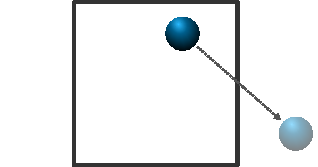
\includegraphics[width=1.3\linewidth]{figures/BoundaryConditions/no.pdf} 
	\\*
	\vspace{0pt} {\it Reflecting boundary conditions}, which act as hard walls. Instead of passing through the boundary, the velocity component in the direction normal to the face of the boundary changes sign, thus causing the atoms to be confined within the simulation box. 
	& \vspace{0pt} \hspace*{-1.3cm} 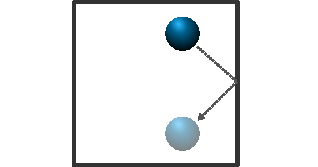
\includegraphics[width=1.3\linewidth]{figures/BoundaryConditions/reflecting.pdf} 
	\\*
	 \vspace{0pt} {\it Periodic boundary conditions}, which allow atoms on separate sides of a boundary to interact through the boundary as if they were neighbors, and atoms crossing the boundary reappears on the other side of the simulation box. This is useful when studying bulk atoms of a material or materials that has a periodic structure.
	& \vspace{0pt} \hspace*{-1.3cm} 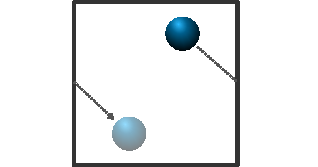
\includegraphics[width=1.3\linewidth]{figures/BoundaryConditions/periodic.pdf}
\end{tabular}
\vspace{10mm}

\noindent
The boundary conditions may include more details than only how to handle the trajectory of atoms intersecting the boundaries. 
For instance, with periodic boundaries atoms that are far apart are effectively close. 
These atoms should therefore interact, since their motion would seem artificial otherwise. 
Thus, the interpretation of atoms positions must in some cases be included in the boundary conditions. 
In order to interpret atoms positions in the case of periodic boundaries, one has to remember that an atom should not interact with multiple images of another atom. 
Which image, if not the original, must therefore be decided. 
Also, an atom should not interact with an image of itself. That could potentially cause strange correlations. 
The standard way of determining atoms positions is by using the {\it minimum image convention}.


\subsection{Minimum image convention}
The minimum image convention simply states that the periodic image of an atom closest to the reference atom is the one to consider as its position. 
Example cases of 1D and 2D systems are shown in figure \ref{fig:minimumImageConvention1D} and figure \ref{fig:minimumImageConvention2D} respectfully. 
In the examples we look at systems consisting of two atoms and we try to determine the minimum image of the smaller, blue atom with respect to the larger, red, reference atom. 
The original system is distinguishable from the periodic copies by the background color; they have a slightly darker background. 
Also, we only bother showing the periodic copies of the atom of consideration, the blue one.  
The systems depicted are of size $L$ and $L\times L$ in the 1D and 2D cases respectfully.

By studying figure \ref{fig:minimumImageConvention1D} it becomes apparent that if the atom of consideration is closer to the reference atom than half the system length, the original image will be used to interpret its position. 
Otherwise, if it's farther apart than half the system length, a periodic image will be closer and therefor used as the atoms position.  
%Mathematically we can deduce that the position of the minimum image can be found as
%\begin{align}
%	\vec{r}_{ij}  = 
%	\begin{cases}
%	\vec{r}_{ij} - L, & \vec{r}_{ij} > L/2 \\
%	\vec{r}_{ij} + L, & \vec{r}_{ij} < -L/2
%	\end{cases}
%\end{align}  
This principle is applicable at higher dimensions as well. We simply decompose the positions and check each dimension separately. For a system of arbitrary number of dimensions the minimum image convention is assured by using the progression of lisiting \ref{mic}. 
Figure \ref{fig:minimumImageConvention2D} illustrate how we decompose the positional separation of the atoms in the 2D case.

\begin{lstlisting}[caption={Loop to compute the position of the closest periodic image of atom $j$ with respect to the referance atom $i$.}, label={mic}, language=c++]
for (int k=0; k<numberOfDimension; k++){
	delta[k] = atom[j].pos[k] - atom[i].pos[k]
	if (delta[k] > L/2) {
		delta[k] = delta[k] - L
	}
	else if (delta[k] < -L/2){
		delta[k] = delta[k] + L
	}
}
\end{lstlisting}

\begin{figure}[H]
	\centering{
		\def\svgwidth{\linewidth}
		\input{figures/minimumImageConvention/1D_2.pdf_tex}
		\caption{Minimum image convention in 1 dimension. 
		If an atom is separated from the reference atom (red) by more than half the system length, $L/2$, the minimum image convention states that the distance between the two is the distance to the periodic copy, which is $|\Delta x - L|$. 
		The white area indicates the system, while the gray areas are periodic replications of the system. Atoms in the gray areas are periodic images of the atom of consideration in the white area.}
		\label{fig:minimumImageConvention1D}
	}
\end{figure}

\begin{figure}[H]
	\centering{
		\input{figures/minimumImageConvention/2D_2.pdf_tex}
		\caption{Minimum image convention in 2 dimensions.
			The position of an atom, with respect to the reference atom (red), is the position of the original or any of the replicated images that has the shortest distance to the reference atom. 
			The minimum image is found by decomposing the atoms position, and carry out the 
			The shortest distance in this case is marked with an arrow. 
			Thus, when computing positional dependent quantities, it's the position of the north-west replica that will be considered as the position of the blue atom in this case.}
		\label{fig:minimumImageConvention2D}
	}
\end{figure}

\section{Measuring physical quantities}
\subsection{Energy}
In molecular dynamics we sample kinetic energy classically as
\begin{equation}
	E_K = \frac{1}{2}mv^2.
\end{equation}
The potential energy is off course dependent on the potential force field in use $U$, and is computed as 
\begin{equation}
	E_P = \sum_{i=1}^{N}\sum_{j>i}^{N}U(\vec{r}_i, \vec{r}_j).
\end{equation} 

\subsection{Temperature}
From thermodynamics we have that the kinetic energy, or total thermal energy is 
\begin{equation}
E_k = \frac{f}{2} Nk_bT, 
\end{equation}
for a system of $N$ atoms with $f$ kinetic degrees of freedom and temperature $T$.  
$k_b$ is the Boltzmann constant. 
Since we assume point particles, we take only the translational degrees of freedom into account and ignore the rotational degrees of freedom.
If we assume Newtonian motion, the total kinetic energy in the system is found as
\begin{equation}
E_k = \frac{1}{2}\sum_{i=1}^{N} m_i {\vec{v}_i}^2.
\end{equation}
We can equate these to find the instantaneous temperature given as
\begin{equation}\label{eq:MDtemperature}
T = \frac{\langle m_i \vec{v_i}^2\rangle}{fk_b}.
\end{equation}
Thus, we can approximate the instantaneous temperature using the atoms velocities.
This value will fluctuate about the real value, so time-averaging is often used when measuring.
In many cases it is desirable to control the temperature of the system, e.g. when using the canonical ensemble (NVT).
Methods for doing this are called \textit{thermostats}, and are described in section \ref{sec:thermostats}.


\subsection{Pressure}
There are many methods for computing the pressure of the system. 
Normally for a N-body system of volume $V$ and particle density $\rho=N/V$ it is taken from the virial equation for pressure. 
\begin{equation}
	P = \rho k_B T + \frac{1}{dV}\Big< \sum_{i<j} \vec{F}_{ij} \cdot \vec{r}_{ij}\Big> 
\end{equation}
where $d$ is the number of dimensions, $\vec{F}_{ij}$ is the force contribution on atom $i$ from atom $j$ positioned at $\vec{r}_{ij}$ relative to atom $i$.
In this expression for the pressure we assume constant $N$,$V$ and $T$, i.e. the canonical ensemble.
The equation will not be the same for the micro-canonical ensemble.
There are methods for converting averages from one ensemble to another \cite{Lebowitz}, but that is outside the scope of this thesis.


\section{Thermostats}\label{sec:thermostats}
Often, we want to control the temperature of our simulated system.
This is done by fixing the temperature in equation \eqref{eq:MDtemperature} and manipulate the atoms velocities.
There are several methods of manipulating the velocities, and these are called \textit{thermostats}. 
There are many different types of thermostats, and they all have their strengths and weaknesses.

We will look at two quite basic and different thermostats, as well as one that is common in professional use.   


\subsection{Berendsen}
The Berendsen thermostat rescales the velocity of all atoms in the system so that the temperature approaches that of the surrounding heat bath.
It rescales the atoms velocity by multiplying them by a scaling factor $\gamma$, given as 
\begin{equation}
\gamma = \sqrt{1+\frac{\Delta t}{\tau}\lr{\frac{T_{bath}}{T}-1}},
\end{equation}
where $\Delta t$ is the time step length, and $\tau$ is a relaxation time, which tune the coupling to the heat bath. 
$T_{bath}$ and $T$ is the temperature of the heat bath and the current temperature of the system, respectfully.
Typically the relaxation time is set to $\tau \approx 20\Delta t$. 
Using $\tau = \Delta t$ would result in the velocities rescaling so the temperature would be exactly the target temperature, $T_{bath}$, every time step. 
This thermostat suppresses temperature fluctuations efficiently, rendering it well suitable for equilibration procedures.
However, because it rescales the velocities, it produces dynamics that are inconsistent with the canonical ensemble.



\subsection{Andersen}
The Andersen thermostat simulates the coupling between the system and an imaginary heat bath as collisions between their atoms. 
Atoms that collide are assigned a new normally distributed velocity with standard deviation  $\sqrt{3k_BT_{bath}/m}$ about the target temperature, $T_{bath}$.
The procedure of the thermostat goes as follows:
For each atom in the system, we generate a random uniformly distributed number in the interval $[0,1]$. 
If this number is less than $\Delta t/\tau$, the atom is considered to be colliding, and is assigned a new velocity. 
Here $\tau$ is regarded as a collision time, and its value should be similar to $\tau$ in the Berendsen thermostat ($20\Delta t$). 
The Andersen thermostat is useful when equilibrating systems, but because randomly chosen particles are assigned randomly distributed velocities, it disturbs the dynamics of e.g. lattice vibrations. 
Also, this disturbance will decorrelate the system, rendering this thermostat ill-equipped when measuring e.g. diffusion coefficient.  
As a final note, if this thermostat is to be used, the newly assigned velocities may cause the systems center of mass to drift.


\subsection{Nosé-Hoover}
The most widely used thermostat is the Nosé-Hoover thermostat. 
It produces  accurate dynamics and realistic constant temperature conditions. 
This thermostat differs from the Berendsen and Andersen thermostats in that it does not rescale the velocity of atoms. 
Instead it alters the hamiltonian of the system by adding a fictitious force of friction.
The equation of motion is changed to
\begin{equation}
	\vec{F}_i = -\nabla U_i(\vec{r}^N) -\zeta m\vec{v_i} ,
\end{equation}    
where $\zeta$ is a dynamic variable determining the strength of the thermostat. 
Due to this change, the integration scheme also has to be altered. 
As the details of this thermostat is somewhat extensive, I recommend reading \textit{Understanding Molecular Simulation} by Frenkel \& Smit \cite{understandingMolecularSimulationFrenkelSmit} for detailed derivation and explanation.

\section{Efficiency improvements}
The major part of the CPU time is spent in the force loop. 
At every time step we must recompute the force acting on each individual atom. 
When doing so, we should in theory include the contribution from all other atoms. 
Having a system consisting of $N$ atoms would result in $N(N-1)/2 \propto N^2$ computations, if we apply Newton's third law.
In this section we will look at the most fundamental efficiency improvements applied in molecular dynamics simulations.

\subsection{Cut-off}
Depending on the potential in use, the forces become negligible at certain distances. 
For instance if one uses the Lennard-Jones potential (introduced in section \ref{Lennard-Jones-section}) the contributions are practically zero for atoms positioned at a distance $r\geq2.5\sigma$.
Therefore, during a simulation we choose to only account for the contributions from atoms closer than this \textit{cut-off} distance, denoted $r_c$.  
%Atoms within the cut-off length from the atom of consideration are referred to as \textit{neighbor atoms}.
For the Lennard-Jones potentials the cut-off range is usually set to $2.5\theta$. 
Past this range, the pair-potential is practically zero. 
It's not zero, though. 
Without any alterations, particles intersecting the cut-off limit will experience an unphysical jerk, which may render the simulation unstable.  
To counteract this effect, we raise the potential, ensuring it and its derivative to be zero at the cut-off. 
We use the following adjustment.

\begin{equation}
	V(r) = 
	\begin{cases}
		\left.V(r) - V(r_c) - \frac{\partial V(r)}{\partial r}\right\rvert_{r=r_c} (r-r_c) &, r\leq r_c \\
		0 &, r>r_c 
	\end{cases}
	\label{eq:truncation}
\end{equation}
which implies the force
\begin{equation}
F(r) = 
\begin{cases}
F(r) = F(r) - F(r_c) &, r\leq r_c \\
0 &, r>r_c 
\end{cases}
\end{equation}
In practice we need to keep track of which atoms are within the cut-off range of each atom. 
This is achieved using cell lists and neighbor lists. 

\subsection{Cell lists and neighbor lists}
The main purpose of the cell list is to make the building of neighbor lists more efficient. 
We need to check which atoms are neighboring atoms, but obviously we do not need to check the entire domain, since the cut-off length is relatively small. 
Therefore, we partition the system into several cubes of size equal to the cut-off length. 
We store the atoms contained by each cell in a \textit{cell list}. 
Finally, when we build the neighbor lists we check only the atoms within the neighboring cells and those in the same cell, 27 cells in total. 
In this sense, by neighboring cells we mean any cells that share a face, edge or vertex. 
This is illustrated in figure \ref{fig:neighbourcells}.
The pay-off of using cell- and neighbor lists is tremendous. Since we now, for each atom, only include contributions from atoms within a constant volume of size $4\pi {r_c}^3/3$, 
the number of contributions will only depend on the density, which is an intensive\footnote{Physical property of a system that does not depend on the system size.} property. 
Thus, the number of computations is reduced to $\mathcal{O} (N)$, which is an immense relief in computational expense!

\begin{figure}
	\center
	\resizebox{0.45\linewidth}{!}{
		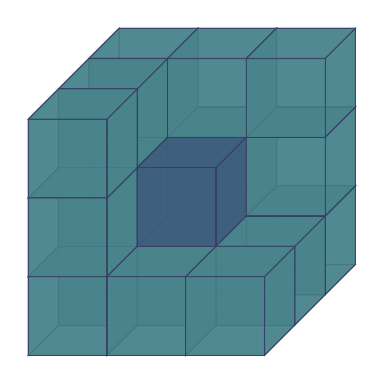
\begin{tikzpicture}

\definecolor{p0}{HTML}{d7dfc0}
\definecolor{p1}{HTML}{aecfa2}
\definecolor{p2}{HTML}{82bc92}
\definecolor{p3}{HTML}{5fa38e}
\definecolor{p4}{HTML}{49848b}
\definecolor{p5}{HTML}{3f5f7f}
\definecolor{p6}{HTML}{383d65}
\definecolor{p7}{HTML}{2c1e3e}

\newcommand{\translatepoint}[1]%
{   \coordinate (mytranslation) at (#1);
}



\newcommand{\drawCube}%
{   
	\coordinate (O) at (0,0,0);
	\coordinate (A) at (0,1,0);
	\coordinate (B) at (0,1,1);
	\coordinate (C) at (0,0,1);
	\coordinate (D) at (1,0,0);
	\coordinate (E) at (1,1,0);
	\coordinate (F) at (1,1,1);
	\coordinate (G) at (1,0,1);
	
	\draw[p6,fill=\cubeColor, opacity=\myO] (O) -- (C) -- (G) -- (D) -- cycle;% Bottom Face
	\draw[p6,fill=\cubeColor, opacity=\myO] (O) -- (A) -- (E) -- (D) -- cycle;% Back Face
	\draw[p6,fill=\cubeColor, opacity=\myO] (O) -- (A) -- (B) -- (C) -- cycle;% Left Face
	\draw[p6,fill=\cubeColor, opacity=\myO] (D) -- (E) -- (F) -- (G) -- cycle;% Right Face
	\draw[p6,fill=\cubeColor, opacity=\myO] (C) -- (B) -- (F) -- (G) -- cycle;% Front Face
	\draw[p6,fill=\cubeColor, opacity=\myO] (A) -- (B) -- (F) -- (E) -- cycle;% Top Face
}

\newcommand{\cubeColor}{p4}
\newcommand{\myO}{0.5}

\foreach \x in {0,1,2}{
	\foreach \y in {0,1,2}{
		\foreach \z in {0,1,2}{
			\ifthenelse{\x=0 \OR \y=0 \OR\z=0}
				{
					\renewcommand{\cubeColor}{p4}
					\renewcommand{\myO}{0.8}
				}
				{
					\renewcommand{\cubeColor}{p4}
					\renewcommand{\myO}{0}
				}
			\ifthenelse{\x=1 \AND \y=1 \AND \z=1}
				{
					\renewcommand{\cubeColor}{p5}
					\renewcommand{\myO}{0.9}
				}
				{}
			\translatepoint{\x,\y,\z}
			\begin{scope}[shift=(mytranslation)]
			\drawCube
			\end{scope}
		}
	}
}



\end{tikzpicture}
	}
	\caption{Illustrative figure of cells of concern when building the neighbor lists. The lighter cubes are considered neighboring cells; the darker cube is the cell containing the reference atom. The 7 cells in front of the dark cell are removed from the figure, but are also included. }
	\label{fig:neighbourcells}
\end{figure}




\subsection{Parallelization}
It might be misguiding to refer to parallelization as an efficiency improvement, when on the contrary it most likely increases the CPU time usage. 
However, the real time consumed may be greatly decreased. 
It is intuitive that partitioning the work and processing these simultaneously will decrease the time as compared to processing it serially.   
The speedup is defined as 
\begin{equation}
S = \frac{T_s}{T_p},
\end{equation}
where $T_s$ is the time used when executing the program on a single processor, and $T_p$ the time used when running on $p$ processors simultaneously.
The time spent running a parallel implementation of a code using $p$ processors is seldom trivially $T_p=T_s/p$. This is due to the fact that there is a certain amount of time used on \textit{overhead}. This includes interprocess communications, idling and excess computations.
In molecular dynamics simulations there is communication between processors when building the cell- and neighbor lists, and when computing thermodynamical properties such as energy, pressure, temperature, etc.. 

During this project we have mainly been using the local supercomputer at the department of physics at the University of Oslo. It provides users with the possibility to run  up to 256 processes at once. Though, before doing so, it is considered as good practice to check the speedup obtained by using several numbers of cores.
In order to compute the speedup, we initialized a system containing $15\times15\times15$ unit cells of beta-cristobalite and saved it as a restart file. 
We then remotely ran the input script shown in Listings \ref{lst:speedup} from the supercomputer using 1, 2, 4, 8, 16, 32 and 64 processors in the same fashion as shown in Listing \ref{speeduprun}.  
The resulting speedup of using the respective number of processors is plotted in figure \ref{fig:speedup15x15}.

\lstinputlisting[caption={LAMMPS input script executed using several numbers of processors, and timed separately.}, label={lst:speedup}]{../SiO2/small/continue.in}

\begin{lstlisting}[caption={Command used to excecute the input script speedup.in on 8 parallel processors and set the filename variable to speedup.restart.}, label={speeduprun}, language=c++]
mpirun -n 8 lmp_mpi -in speedup.in -var filename speedup.restart
\end{lstlisting}
\begin{figure}[H]
	\centering
	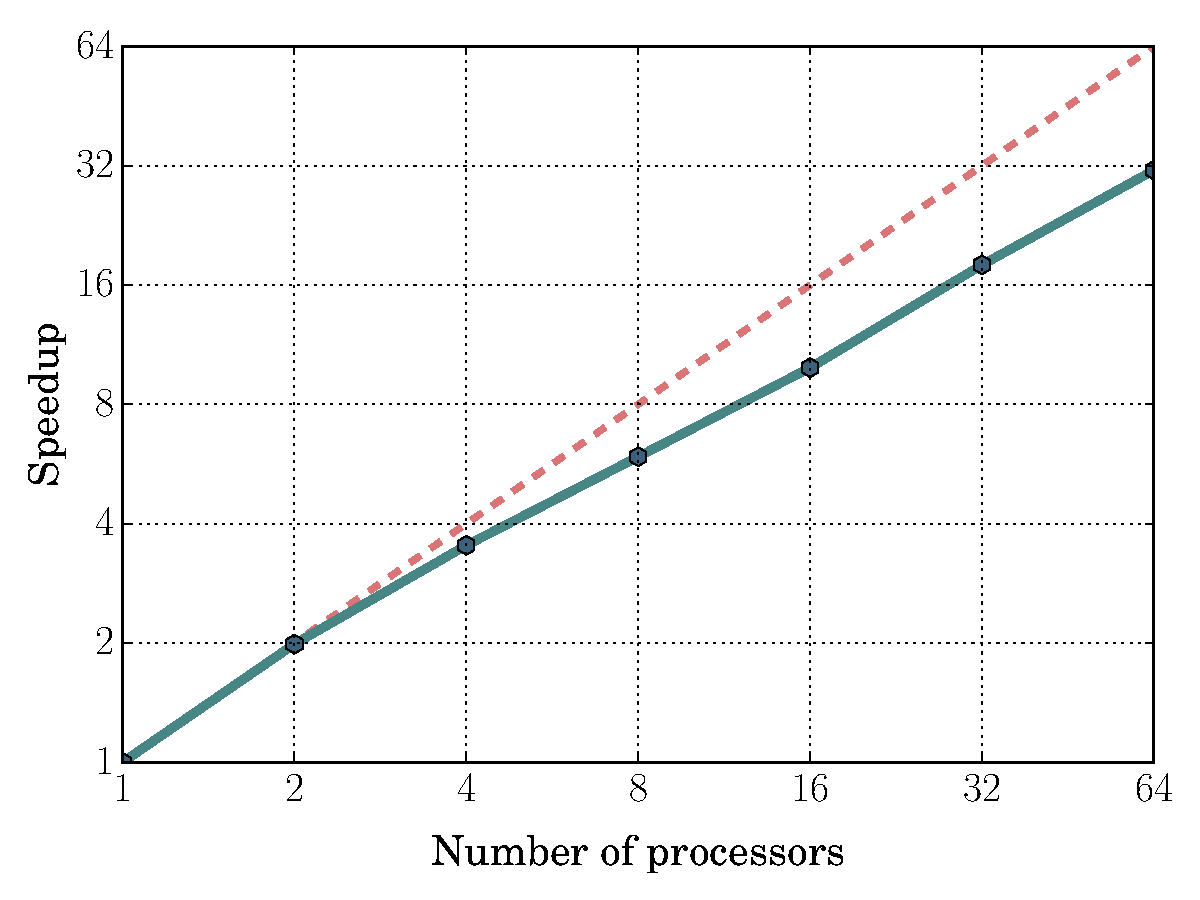
\includegraphics[width=0.7\linewidth]{figures/speedup/15x15_bigFonts.pdf}
	\caption{Strong scaling of parallel performance of LAMMPS using 81000 atoms, evenly distributed in a cubical simulation box. The marked points are measured speedup, while the dashed line represents ideal speedup ($S = T_s/T_p = p$). }
	\label{fig:speedup15x15}
\end{figure}




The result indicate that the speedup is in fact not simply $S=p$. 
Nevertheless, we clearly see the advantage of using 64 processors in parallel as opposed to a single processor serially. 
We can finish a job that would have taken an hour in two minutes!
Also, we clearly see that the initial claim holds; this is not more efficient when regarding CPU time. 
In fact this result suggest that using 1 processor is twice as energy efficient as using 64. 


\chapter{Friction, elasticity and contact mechanics}
Friction can be defined as \textit{the force that resists relative motion between two bodies in contact} \cite{frictionDefinition}. 
It's a well-known phenomenon, though still not completely understood.
Despite the fact that we learn about friction in introductory courses to physics, it is not at all easy to comprehend. 
It's very complex and still a field of research.
The effects of friction is affected by surface roughness, material properties, ambient conditions, the geometry of contact area, and many other factors. 
In this chapter we will study some elementary aspects of dry friction between two solid bodies, elasticity and contact mechanics. 
   
 
\begin{figure}[H]
	\centering
	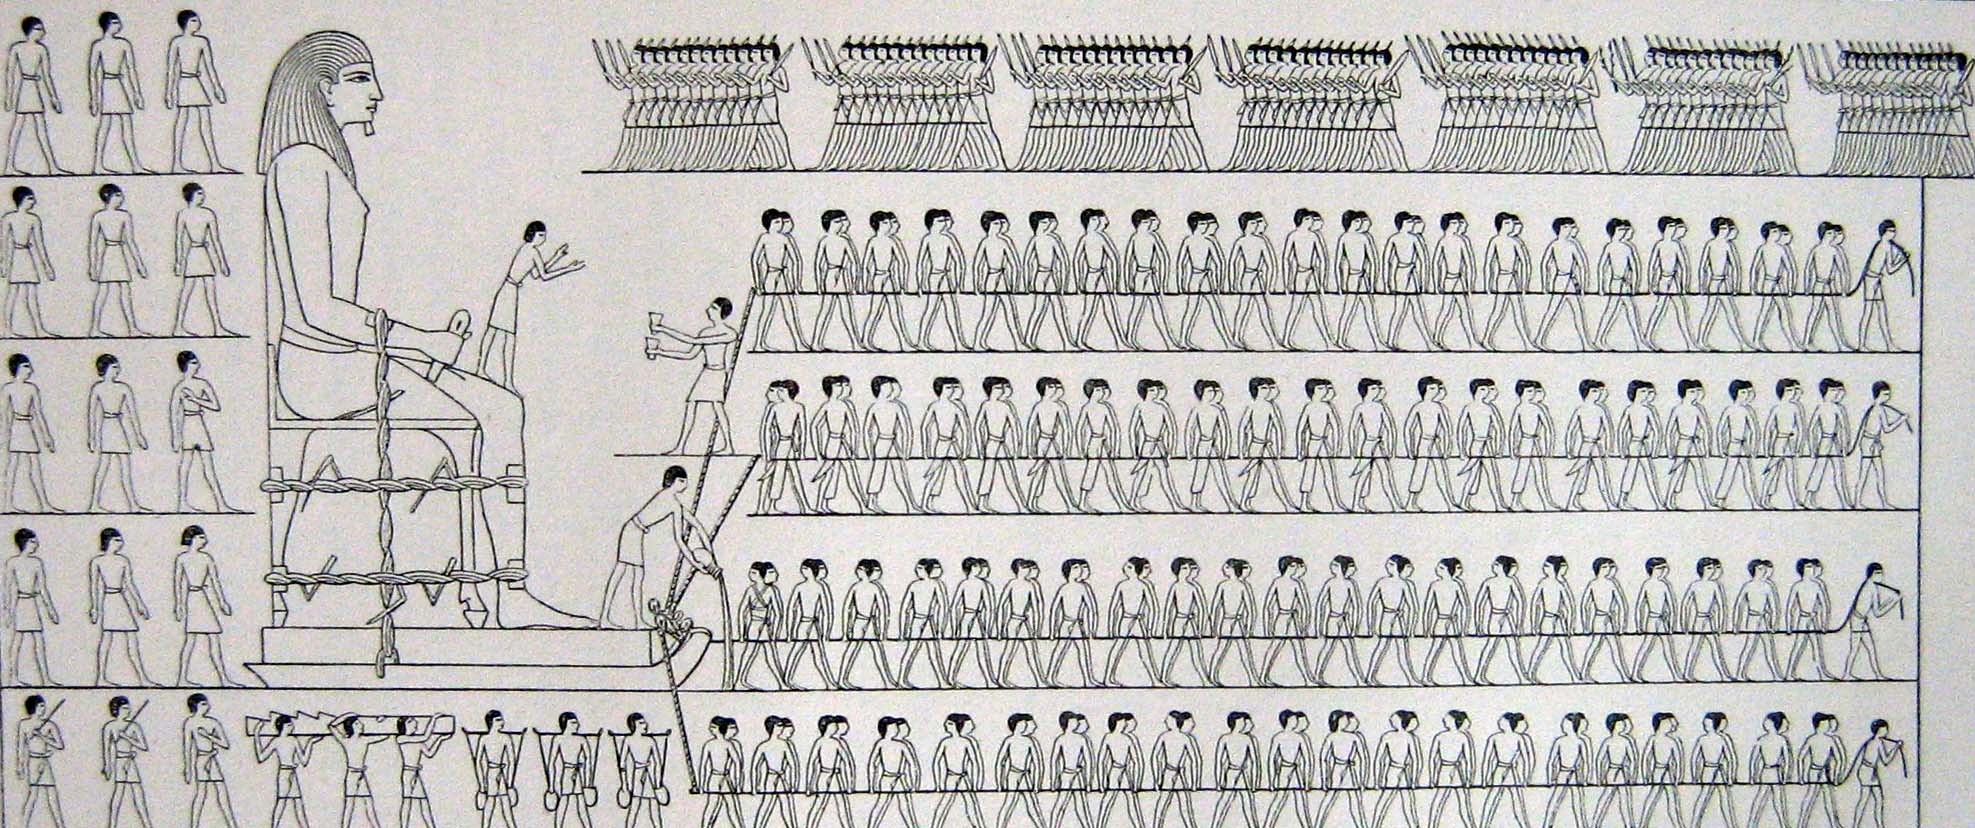
\includegraphics[width=0.99\linewidth]{figures/friction/Colossus.jpg}
	\caption{Painting from the tomb of Tehuti-Hetep, showing the transportation of an Egytian colossus.}
	\label{fig:Colossus}
\end{figure}
\section{Historical note}
On the macroscopic level, friction has been observed since the dawn of man. 
Early actions that show awareness of the effects of friction was to chip stone in order to make tools, or rubbing wood in order to create fire. 
In the tomb of Tehuti-Hetep there was found the painting shown in figure \ref{fig:Colossus}, which show the moving of an Egyptian colossus. 
The statue is depicted pulled on a sledge, with officers standing on the front end of the sledge pouring water on the ground. 
This is evidence that they perceived the effect of lubrication even then, 1900 B.C..   


\begin{figure}[H]
	\centering
	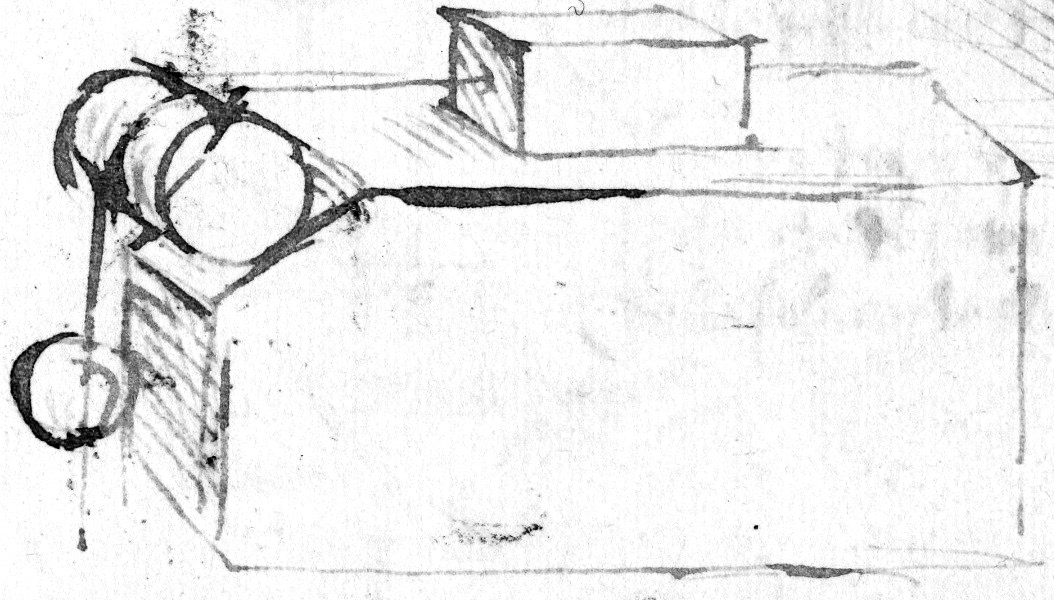
\includegraphics[width=0.5\linewidth]{figures/friction/LeonardoDaVinciBW}
	\caption{Drawing from Leonardo da Vinci's notebook. From Codex Arundel, British Library, London (Arundel folio 41r).}
	\label{fig:leonardoDaVinci}
\end{figure}


\noindent 
The first documented studies of friction were carried out during the renaissance by Leonardo da Vinci (1452-1519) \cite{LeonardoDaVinciStudies}.
Among his experiments he attaching a block of wood to another object with a cord, and placed the block on a smooth surface.
He was able to adjust the weight of the second object, which he let hang over a fixed cylinder, free to rotate. 
This experiment was found in his notebooks, and is shown in figure \ref{fig:leonardoDaVinci}.
He experimented with tilted planes and placed the block on different sides, changing the apparent area of contact.
His results made him deduce the following statements, also found in his notes:
\begin{itemize}
	\item Friction produces double the amount of effort if the weight be doubled. 
	\item Friction made by the same weight will be of equal resistance at the beginning of the movement though the contact may be of different breadths or lengths.
\end{itemize}
This is now essentially known as the two first laws of friction. 
They were not recognized at the time, but were rediscovered later by Guillaume Amontons, and these laws of friction are most commonly known as \textit{Amontons' laws}.
The linear relation described in the first postulate is commonly known as the coefficient of friction
\begin{equation}
	\mu = \frac{F}{L}, \label{eq:coefficientOfFriction}
\end{equation}
though Leonardo interpreted $L$ as the weight of the load and $F$ as the weight of the object pulling in a scenario as in figure \ref{fig:leonardoDaVinci}. The concept of force was not commonly recognized until 200 years later. Isaac Newton's publication of \textit{Principia} paved the way for studies of friction, there among the most comprehensive study carried out by Charles Augustin Coulomb (1736-1806). He investigated the influence of several factors on friction, namely \cite{SlidingFriction}:
\begin{itemize}
	\item The nature of the materials in contact and their surface coatings.
	\item The extent of the surface area.
	\item The normal force.
	\item The amount of time that the surfaces remained in contact prior to the applied force.
	\item Ambient conditions.
\end{itemize}   
Among his results he found that the static friction force increased with the time the surfaces were in contact before applying shear force. 
Today this relation is known as
\begin{equation}
	F_s(t) = A+B\ln(t).
\end{equation}
Coulomb explained this behavior by regarding the materials as fibrous. 
Basically like a hairbrush, having fibers which get entangled into a mesh when in contact. 
If the materials were in contact over a short period of time, fewer fibers would have gotten into their position in the mesh. 
When a shear force is applied, the fibers get tilted until they loosen from the mesh, at which point sliding occurs. 
This impression of the sliding mechanism is quite similar to the one we have now. 




\section{Macroscopic observations}

%There are two fundamental forces that cause the friction force: gravitational force and electromagnetic force. 



\subsection{Coefficient of friction}\label{sec:coefficientOfFriction}
The coefficient of friction, $\mu$, is a dimensionless scalar describing the ratio between the force of friction and the normal force, as given in equation \eqref{eq:coefficientOfFriction}.
The value of $\mu$ is dependent on the material of the objects that are in contact, ambient conditions, presence of lubrication, etc.. 
For most materials the coefficient is higher if the objects are stationary, than if they are moving relative to each other (sliding).
We may refer to them separately as the coefficient of static friction $\mu_s$, and the coefficient of kinetic friction $\mu_k$.
Thus, $\mu_s>\mu_ k$ for most materials\footnote{Teflon-on-teflon seems to have the same value for static- and kinetic friction.}.

\subsection{Steady sliding}
If we attach a spring to a block and pull on the spring with a constant velocity, we may get the evolution of friction force as shown in figure \ref{fig:steadyslide}.
We assume the block to have a constant normal force from the surface it rests upon. 
We observe that the friction force increases linearly during the loading of the spring, as expected from Hooke's law. 
Once the force from the spring overcomes the maximum static friction , $F_s$, the block begins to move (slide) and the force of friction is reduced due to the change in coefficient of friction. 
The coefficient of static friction is found by using the maximum static friction force, $F_s$, in equation \eqref{eq:coefficientOfFriction}. 
Similarly the coefficient of sliding friction is found by using the value of the friction force in the sliding domain, $F_k$.
In this scenario, the motion of the block resulted in a steady motion. 
As we shall see, that is not always the case.

Keep in mind that the forces we refer to are considered to be working on the center of mass of the block. 
The coefficient of friction is a macroscopic observation.
It wouldn't make any sense to discuss a coefficient of friction between let's say two "blocks" containing 10 atoms each.
How would one even define a normal force? 

Steady sliding motion can be observed for instance if a car driver pulls on the break at high speed, so that the wheels are unable to turn.
The wheels will then slide along the road until the car comes to a stop. 
At cites of traffic accidents it is common to measure the length of skid marks, in order to approximate a lower limit of a vehicles velocity. 


\subsection{Stick-slip motion}
If we pull on a body with a spring with constant and reasonably low velocity, it will be subject to a linearly increasing force (Hooke's law). 
Because the object does not slide until we reach the maximum static friction, it will remain its position until it does.
Once the force from the spring overcomes the maximum static friction, the body will begin to slide and the coefficient of friction changes to its kinetic state.
It will accelerate the most in the beginning, and continue increasing its velocity until it passes an equilibrium position.
Once it passes the equilibrium position, the friction force will overcome the spring force, and the velocity will decrease. 
When the velocity is sufficiently low, the object will stop abruptly. 
As the spring is still being moved, the spring force on the object will rise again (load), and we have a complete cycle.
The time evolution of the force applied by the spring will be similar to the sketch shown in figure \ref{fig:stick-slip}.
If the surface of the block or substrate is non-homogeneous, the stick-slip motion may be more chaotic, than illustrated by the sketch. 
In fact, it may be difficult to find any periodicity in the motion at all. 
We are not going to concern our self with chaotic stick-slip motion, since we will have perfectly smooth, dry and pure surfaces when doing molecular dynamics simulation.  
Stick-slip motion can be observed for instance when a bow slides over the strings of a violin, thus making them vibrate. 
By changing the pressure and speed of the bow, the performer can modify the sound produced. 
Earth quakes is another example, though this is of the chaotic sort.

Whether the motion is of the steady type or the stick-slip type, is found experimentally to be depending on the velocity and  stiffness of the spring.
At sufficiently high speeds, we would always get a steady motion. 
Similarly, with a stiff enough spring we would also get a steady motion. 
While with a velocity, $v<v_s$, and stiffness $k<k_s$ we would expect a stick-slip motion.
This can be illustrated by a phase diagram of velocity and spring stiffness $(v,k)$, as in figure \ref{fig:phase-stick-slip}.
The change in behavior from stick-slip to steady motion can be observed in our daily lives. 
The creaking of a door is due to stick-slip motion at the hinges.
However, if we open the door quickly, the door will not creak.
  
%The sound produced by bowed instruments such as the cello or violin are dependent of the speed at which the bow is drawn across the strings. 
 
 \subsection{Microscopic origin of friction}
 Friction is caused by bond formations between atoms of the two bodies, at the area of contact. 
 This includes chemical bonds, hydrogen bonds, dipole-dipole interactions, and so on.  
 The range of these interactions are typically quite short; at 10\AA ~separation they are negligible.
 These bonds oppose relative motion, since the bonds must be broken for sliding to occur.
 As bonds are formed, they have associated energies required for the bonds to be broken. 
 Thus, there is an energy barrier that must be overcome in order for relative motion to initiate,
 which is precisely our observation on the macroscopic level. 
 The bonds can brake either by applying an external force or by thermal excitation\footnote{This is known as \textit{creep}.}.
 The energy released by the braking the bond can be converted into excitation of electrons, creation of phonons, mechanical energy in the form of elastic or plastic deformation, and heat \cite{Introduction2Friction}.
 
 Since the force of friction is due to an activation energy for breaking the bonds, it is intuitive that the force is proportional to the number of bonds
 \begin{equation}
 F \propto N_{\text{bonds}}.
 \end{equation} 
 As the formation of bonds only occur at the area of contact, one would expect $F\propto N_\text{bonds}\propto A$, which violates Amontons' second law. 
 As we shall see in section \ref{sec:contactMechanics}, there is a difference in the \textit{real} area of contact and the \textit{apparent} area of contact.
 
\begin{figure}[H]
	\centering
	\begin{minipage}{\textwidth}
		\centering
		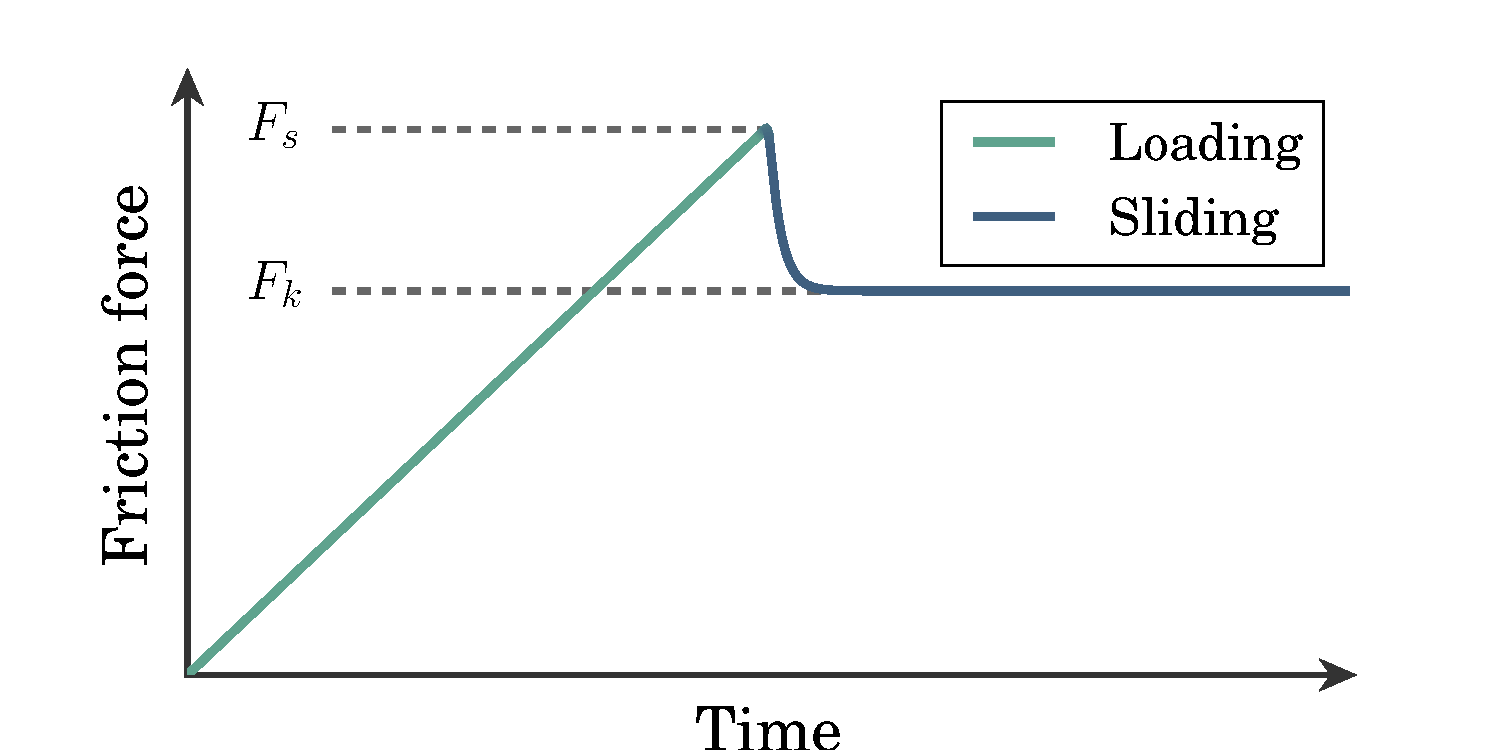
\includegraphics[width=0.7\linewidth]{figures/friction/steadySlide}
		\caption{Behavior of friction force as function of time, for a block pulled at constant velocity and under constant load, resulting in a steady sliding motion.}
		\label{fig:steadyslide}
	\end{minipage}
	\begin{minipage}{\textwidth}
		\vspace{0.5cm}
		\centering
		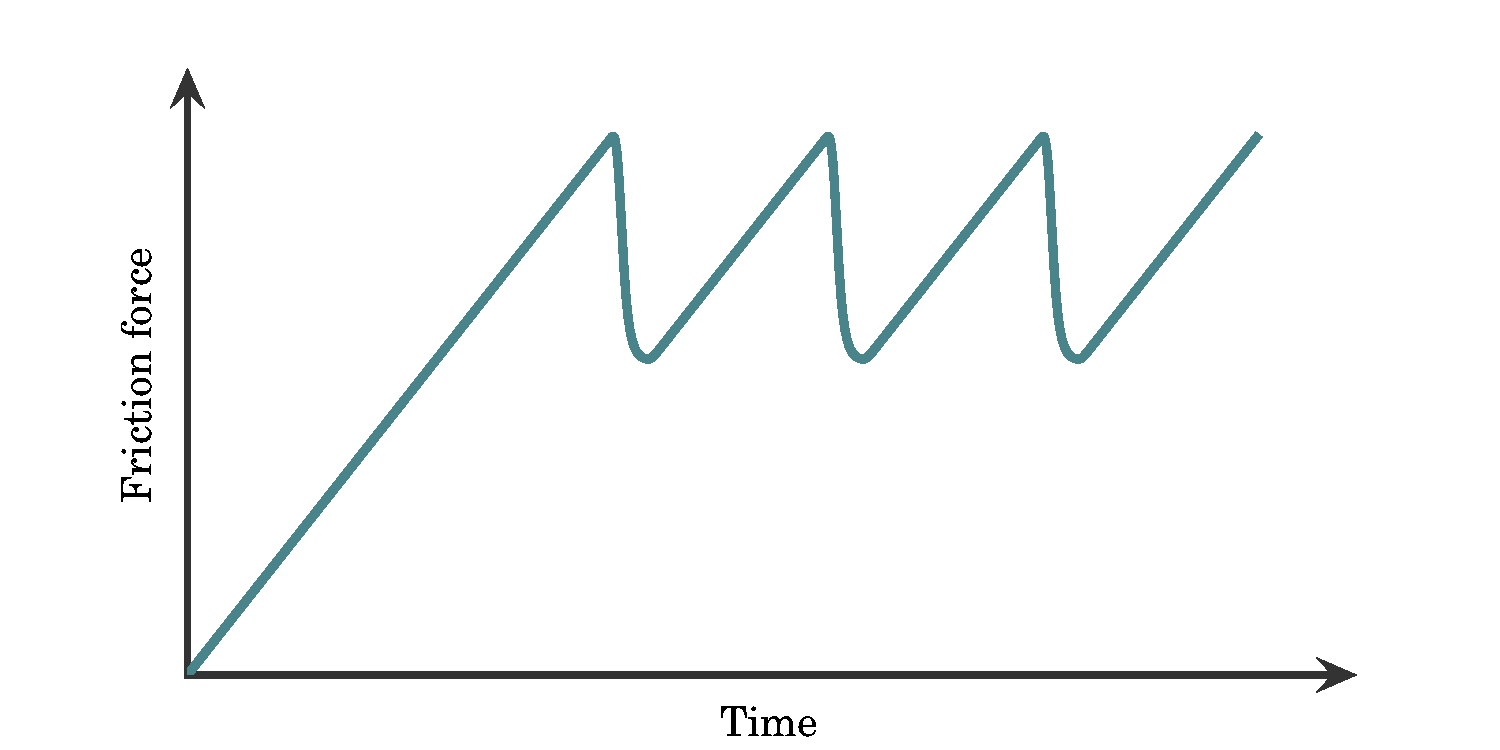
\includegraphics[width=0.7\linewidth]{figures/friction/stick-slip}
		\caption{Behavior of friction force as function of time, for a block pulled at constant velocity and under constant load, resulting in a stick-slip motion.}
		\label{fig:stick-slip}
	\end{minipage}
	\begin{minipage}{\textwidth}
		\vspace{1cm}
		\centering{
			\def\svgwidth{0.58\linewidth}
			\hspace{-3mm}
			\input{figures/friction/phase.pdf_tex}
			\caption{Phase diagram of velocity and spring stiffness ($v,k$). 
				All combinations within the gray area will result in a stick-slip motion. 
				All outside will result in a steady sliding motion.}
			\label{fig:phase-stick-slip}
		}
	\end{minipage}
\end{figure}

%\begin{figure}[H]
%	\centering
%	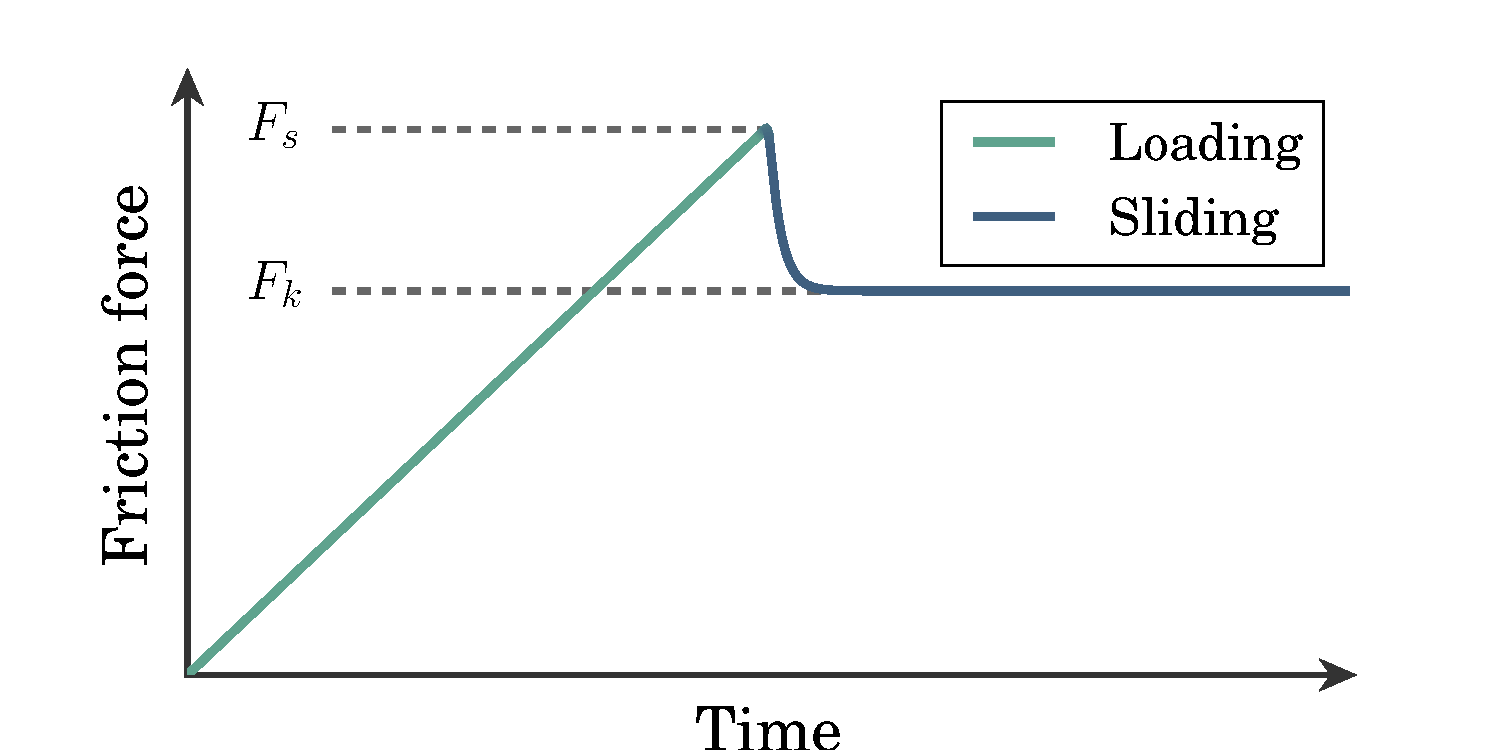
\includegraphics[width=0.7\linewidth]{figures/friction/steadySlide}
%	\caption{Behavior of friction force as function of time, for a block pulled at constant velocity and under constant load, resulting in a steady sliding motion.}
%	\label{fig:steadyslide}
%\end{figure}
%\begin{figure}[H]
%	\centering
%	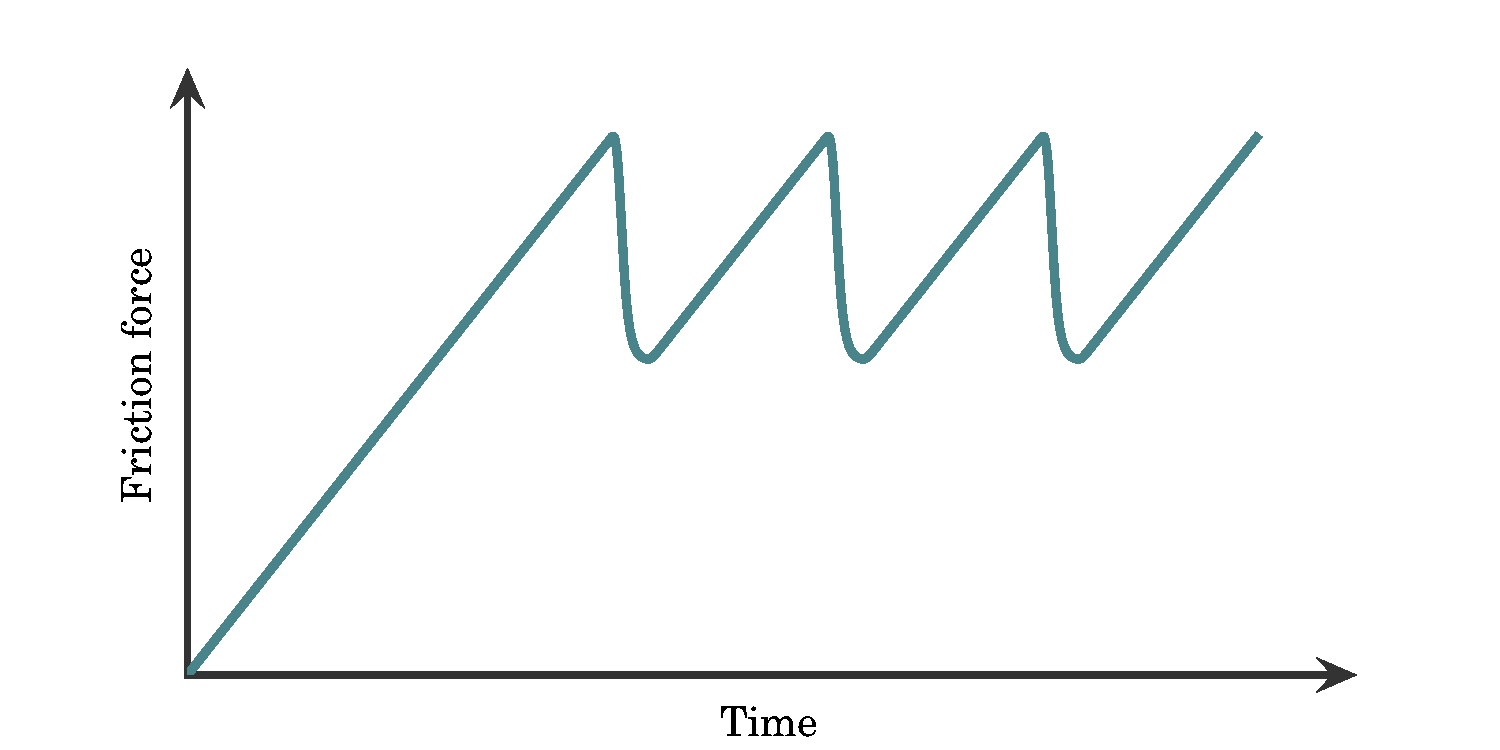
\includegraphics[width=0.7\linewidth]{figures/friction/stick-slip}
%	\caption{Behavior of friction force as function of time, for a block pulled at constant velocity and under constant load, resulting in a stick-slip motion.}
%	\label{fig:stick-slip}
%\end{figure}
%\begin{figure}[H]
%	\centering{
%		\def\svgwidth{0.58\linewidth}
%		\hspace{-3mm}
%		\input{figures/friction/phase.pdf_tex}
%		\caption{Phase diagram of velocity and spring stiffness ($v,k$). 
%			All combinations within the gray area will result in a stick-slip motion. 
%			All outside will result in a steady sliding motion.}
%		\label{fig:phase-stick-slip}
%	}
%\end{figure}





%Bonds will be formed and broken continuously (for temperatures $T>0K$).
%Obviously, the structure of the surfaces and elastic properties also affect the   




%In order to understand the behavior on the macroscopic level, we study the dynamics at a microscopic level as well. 
%As it turns out, there are several similarities and differences between these length scales.






\section{Elasticity}


We distinguish between elastic and plastic deformations.
If a body is deformed by an external force, but recovers its initial structure after the force causing the deformation is removed, it is referred to as an \textit{elastic} deformation. 
If it does not, it is regarded a \textit{plastic} deformation. 
Obviously, there is a limit to the applied stress that separates the two;  the so-called yield stress. 
In this section we will only consider elastic deformations, and review fundamental concepts of linear elasticity. 





\subsection{Strain and stress}
%Imagine a solid cube of some material, e.g. steel.
%At rest, the atoms of the steel is in an ordered structure, having equilibrium distance between each other.
%If a force is applied on the faces of the cube along the  x-axis, toward the center, the cube will deform. 
%It will be compressed in the x-direction. 
%To maintain the cube at the same compression length, we have to retain the compression force constant. 
%This is because the atoms of the cube will be closer than their equilibrium distance from each other in the x-direction, and thus they exert a force outward on the faces of the x-axis.
%If we remove the compression forces, the 
Strain $\epsilon$, is a measure of deformation. 
It represents the displacement between particles in a body relative to a reference length, and can be expressed as
\begin{equation}
	\epsilon = \frac{\Delta l}{l_0}
\end{equation}
where $\Delta l$ and $l$ are the displacement and original length, respectively. 
For \textit{normal} strain, $\Delta l$ represents an elongation of the distance between two facing end planes of an infinitesimal cubic element.
For \textit{shear} strain, it represents a component of an in-plane displacement of the midpoints of said plains.
%It is common to use an index notation in order to describe which component of strain we are referring to.
It is common to discern the components of stress by using two indices, e.g. $\epsilon_{xy}$.
The first index indicates that we consider the planes normal to the x-axis, while the second that we consider the shear stress in the y-direction of these planes. 
Double indices, such as $\epsilon_{xx}$ refer to the normal strain in the x-direction, and is commonly abbreviated to   $\epsilon_{x}$.

Stress $\sigma$, is a force density acting on a body due to internal forces, caused by strain.
For stress on a plane, the \textit{normal} and \textit{shear} stress is defined as
\begin{equation}
	\sigma_\perp = \frac{F_\perp}{A} \qquad \text{and} \qquad \sigma_\parallel = \frac{F_\parallel}{A}
\end{equation}
respectively, where $F_\perp$ and $F_\parallel$ are the force components perpendicular and parallel to the plane.
We use an equivalent notation for stress as for strain, with two indices distinguishing the components.
This is illustrated in figure \ref{fig:stressTensor}.
The collection of stress and strain components are often composed into the so-called Cauchy stress tensor and strain tensor.
\begin{equation}
\sigma = 
\begin{pmatrix}
\sigma_{x} & \sigma_{xy} & \sigma_{xz} \\
\sigma_{yx} & \sigma_{y} & \sigma_{yz} \\
\sigma_{zx} & \sigma_{zy} & \sigma_{z} \\
\end{pmatrix}
\qquad
\epsilon = 
\begin{pmatrix}
\epsilon_{x} & \epsilon_{xy} & \epsilon_{xz} \\
\epsilon_{yx} & \epsilon_{y} & \epsilon_{yz} \\
\epsilon_{zx} & \epsilon_{zy} & \epsilon_{z} \\
\end{pmatrix}
\end{equation}

\begin{figure}
	\center
	\resizebox{0.5\linewidth}{!}{
		%http://latex-community.org/know-how/440-tikz-3dplot

\tdplotsetmaincoords{75}{123}
\begin{tikzpicture}[
		tdplot_main_coords,
		grid/.style={very thin,gray},
		axis/.style={->,blue,thick},
		cube/.style={very thick, fill=black!5, fill opacity=0.9},
		cube hidden/.style={very thick,dashed}]
		%draw the axes
	\draw[axis, very thick, black, dashed] (0,0,0) -- (5,0,0) node[anchor=north east]{\normalsize$x$};
	\draw[axis, very thick, black, dashed] (0,0,0) -- (0,5,0) node[anchor=west]{\normalsize$y$};
	\draw[axis, very thick, black, dashed] (0,0,0) -- (0,0,5) node[anchor=south]{\normalsize$z$};

	%draw the front-right of the cube
	\draw[cube] (4,0,0) -- (4,4,0) -- (4,4,4) -- (4,0,4) -- cycle;
	\draw[axis, very thick, black] (4,2,2) -- (5,2,2) node[anchor=south, inner sep=6]{\normalsize$\sigma_x$};
	\draw[axis, very thick, black] (4,2,2) -- (4,3,2) node[anchor=north, inner sep=5]{\normalsize$\tau_{xy}$};
	\draw[axis, very thick, black] (4,2,2) -- (4,2,3) node[anchor=west]{\normalsize$\tau_{xz}$};
	%draw the front-left of the cube
	\draw[cube] (0,4,0) -- (4,4,0) -- (4,4,4) -- (0,4,4) -- cycle;
	\draw[axis, very thick, black] (2,4,2) -- (2,5,2) node[anchor=north, inner sep=5]{\normalsize$\sigma_y$};
	\draw[axis, very thick, black] (2,4,2) -- (3,4,2) node[anchor=south, inner sep=5]{\normalsize$\tau_{yx}$};
	\draw[axis, very thick, black] (2,4,2) -- (2,4,3) node[anchor=west]{\normalsize$\tau_{yz}$};
	%draw the top of the cube
	\draw[cube] (0,0,4) -- (0,4,4) -- (4,4,4) -- (4,0,4) -- cycle;
	\draw[axis, very thick, black] (2,2,4) -- (2,2,5) node[anchor=west]{\normalsize$\sigma_z$};
	\draw[axis, very thick, black] (2,2,4) -- (3,2,4) node[anchor=south, inner sep=5]{\normalsize$\tau_{zx}$};
	\draw[axis, very thick, black] (2,2,4) -- (2,3,4) node[anchor=north, inner sep=4, pos=0.75]{\normalsize$\tau_{zy}$};
	%draw dashed lines to represent hidden edges
%	\draw[cube hidden] (0,0,0) -- (4,0,0);
%	\draw[cube hidden] (0,0,0) -- (0,4,0);
%	\draw[cube hidden] (0,0,0) -- (0,0,4);
	
\end{tikzpicture}

	}
	\caption{Graphical illustration of the components of the Cauchy stress tensor.}
	\label{fig:stressTensor}
\end{figure}


\subsection{Hooke's law}
As mentioned, stress is caused by strain. However, strain is also caused by stress. 
The relation between the two is known as Hooke's law. 
If we consider a infinitesimal cubical body subject to a tensile force in the x-direction, Hooke's law states that the relation between stress and strain is given as
\begin{equation}
	\epsilon_x = \frac{\sigma_x}{E},
\end{equation}
where $E$ is a material property known as Young's modulus\footnote{Young's modulus is also known as the elastic modulus.}, which express the stiffness of the material. 
Here we assume that the deformation is elastic.
%As the body is expanded in on direction, as in our example, it will experience a contraction in the other two dimensions. 
%These contractions can be expressed as
%\begin{equation}
%	\epsilon_y = -\nu \frac{\sigma_x}{E}, \qquad \epsilon_z = -\nu \frac{\sigma_x}{E},
%\end{equation}
%where $\nu$ is Poisson's ratio.

Often the faces of the infinitesimal cubic body are subject to forces in several direction. 
The general form of Hooke's law is expressed as
\begin{equation}
	\sigma_{ij} = C_{ijkl}\epsilon_{kl}
\end{equation}
which relates the Cauchy stress tensor $\sigma_{ij}$ to the strain tensor $\epsilon_{kl}$, through the linear dependence of the stiffness tensor $c_{ijkl}$.
Note that each component of the Cauchy stress tensor is dependent on all elements of the strain tensor. 
The stress and strain tensors are both of rank 2 and have $3^2=9$ elements, while the stiffness tensor has rank 4 and contains $3^4=81$ elements.
However, since both the Cauchy stress tensor and the strain tensor are symmetric, 
\begin{align}
\begin{split}
	\sigma_{ij} = \sigma_{ji} &\Rightarrow C_{ijkl} = C_{jikl}\\
	\epsilon_{kl} = \epsilon_{lk} &\Rightarrow C_{ijkl} = C_{ijlk}
\end{split}
\end{align}
In total there will be only 6 independent components for the stress and strain tensors, and 36 in the stiffness tensor. 
We may choose to express the stress and strain as vectors by using Voigts method for rank reduction \cite{Voigt}.

\begin{equation}
\vec{\sigma} = 
\begin{pmatrix}
\sigma_{xx} \\
\sigma_{yy} \\
\sigma_{zz} \\
\sigma_{xy} \\ 
\sigma_{xz} \\
\sigma_{yz}
\end{pmatrix}
\equiv
\begin{pmatrix}
\sigma_{1} \\
\sigma_{2} \\
\sigma_{3} \\
\sigma_{4} \\ 
\sigma_{5} \\
\sigma_{6}
\end{pmatrix}
\qquad
\text{and}
\qquad
\vec{\epsilon} = 
\begin{pmatrix}
\epsilon_{xx} \\
\epsilon_{yy} \\
\epsilon_{zz} \\
2\epsilon_{xy} \\ 
2\epsilon_{xz} \\
2\epsilon_{yz}
\end{pmatrix}
\equiv
\begin{pmatrix}
\epsilon_{1} \\
\epsilon_{2} \\
\epsilon_{3} \\
\epsilon_{4} \\ 
\epsilon_{5} \\
\epsilon_{6}
\end{pmatrix}
\end{equation}
Similarly the stiffness tensor reduces to a $6\times6$ matrix (rank 2).
\begin{equation}
	\vec{\hat{C}} = \begin{pmatrix}
	C_{11}& C_{12}& C_{13}& C_{14}& C_{15}& C_{16} \\
	C_{21}& C_{22}& C_{23}& C_{24}& C_{25}& C_{26} \\
	C_{31}& C_{32}& C_{33}& C_{34}& C_{35}& C_{36} \\
	C_{41}& C_{42}& C_{43}& C_{44}& C_{45}& C_{46} \\
	C_{51}& C_{52}& C_{53}& C_{54}& C_{55}& C_{56} \\
	C_{61}& C_{62}& C_{63}& C_{64}& C_{65}& C_{66} \\
	\end{pmatrix}
\end{equation} 
The structure of the elements in the stiffness tensor are dependent on the isotropy\footnote{Directionally dependent physical properties.} of the material of consideration.
The general Hooke's law can now be expressed as a matrix product
\begin{equation}
	\vec{\sigma} = \vec{\hat{C}}\vec{\epsilon}
\end{equation}


\section{Contact mechanics} \label{sec:contactMechanics}


\subsection{Real area of contact}
Today we know that most surfaces are rough, at least at a microscopic level, having some degree of asperities. 
A \textit{contact} is defined as a point where two surfaces meet and where bonds can be formed \cite{Introduction2Friction}.  
It is actually the asperities that make up the contact areas between surfaces.
The real area of contact is therefore the sum of individual contact area of the asperities. 
We can approximate the real area macroscopically. 
Imagine two surfaces initially apart, having no area of contact, as in figure \ref{fig:realAreaOfContact0}. 
The top body has a load $L$ due to its mass. 
It will move downwards, and at some point a single asperity will come in contact with the substrate.
The pressure at the point of contact will be huge, since a single asperity carries the entire load with a very small contact area\footnote{Typical radius of the contact area on an asperities is $\sim10 \mu m$.} of $A_r$.
\begin{equation}
	p = \frac{L}{A_r}
\end{equation}
The pressure will surely be much greater than the yield stress $\sigma_c$, and so the asperity will deform plastically. 
As the surface continues to descend, other asperities will come in contact with the substrate, increasing the contact area and share the load. 
They will all deform plastically until the area of contact is large enough so that the pressure at the points of contact is lower than the yield stress.
At this point the top body is resting on the substrate.
Thus, we should be able to relate the real area of contact to the yield stress as
\begin{equation}
	A_r =  \frac{L}{\sigma_c}.
\end{equation}
At this point it is clear that Amontons' second law is preserved, since 
\begin{equation}
	F\propto N_\text{bonds}\propto A_r \propto \frac{L}{\sigma_c}
\end{equation}
is not dependent on the apparent area of contact. 
In fact we just found Amontons' first law!

As an example\footnote{This example is also found in reference \cite{Introduction2Friction}. } of the difference between apparent and real area of contact, consider a steel plate of size $10cm\times10cm\times1cm$. The apparent area is then $A_a=100cm^2$. Assuming steel to have a density $\rho=10g/cm^3$ and yield stress at $\sigma_c=10^9N/m^2$, the real area of contact is $A_r = 10^{-8}m^2 = 10^{-4}cm^2$.
Thus, there is a huge difference in the apparent and real area of contact, a factor of a million in this case, but only the real area contributes to the effects of friction. 
%When there is contact between two surfaces, the asperities are pushed into the other material, and tries to occupy the position with the lowest potential.  
%The asperities may move even though the macroscopic body is still, due to thermally activated creep.
%Thus, longer duration of resting contact gives a higher rate of asperities that settle in positions with the lowest potential, effectively making the coupling of the bodies stronger.

\begin{figure}
	\centering
	\begin{subfigure}{\textwidth}
		\centering
		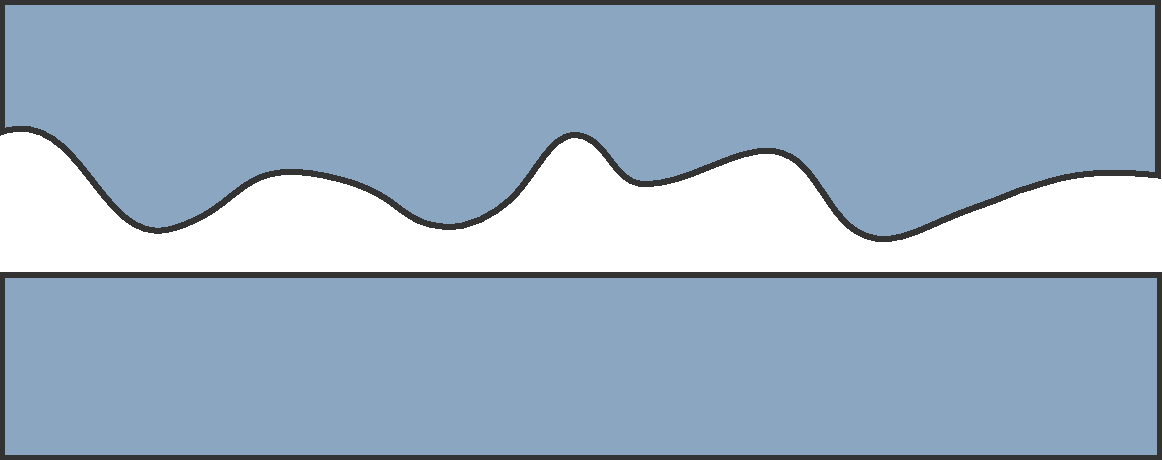
\includegraphics[width=0.5\linewidth]{figures/friction/areaOfContact/apart.pdf}
		\caption{No contact.}
		\label{fig:realAreaOfContact0}
	\end{subfigure}
	\begin{subfigure}{\textwidth}
		\vspace{5mm}
		\centering
		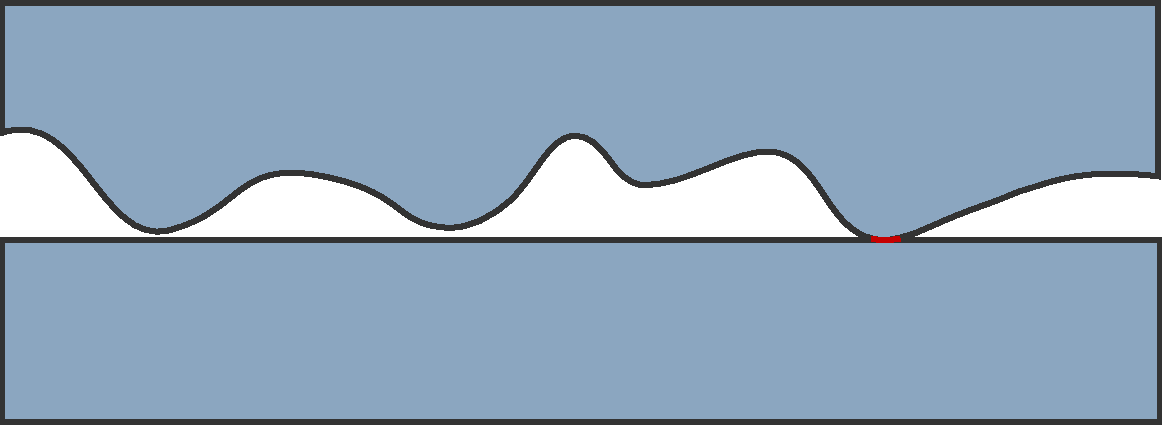
\includegraphics[width=0.5\linewidth]{figures/friction/areaOfContact/single.pdf}
		\caption{Single point of contact.}
		\label{fig:realAreaOfContact1}
	\end{subfigure}
	\begin{subfigure}{\textwidth}
	\vspace{5mm}
	\centering
	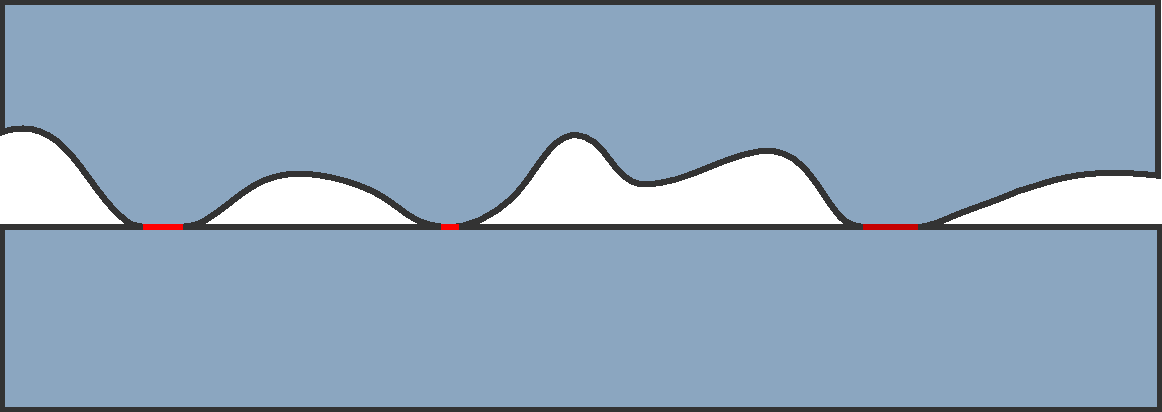
\includegraphics[width=0.5\linewidth]{figures/friction/areaOfContact/three.pdf}
	\caption{Multiple points of contacts.}
	\label{fig:realAreaOfContact3}
\end{subfigure}
\caption{Illustrating the concept of real area of contact, as well as surface roughness. }
\label{fig:realAreaOfContact}
\end{figure}



 
\subsection{Hertz theory}
The first satisfactory analysis of the stresses at the contact of two elastic solids is due to Heinrich Hertz.










\chapter{LAMMPS}

LAMMPS is an acronym for \textit{Large-scale Atomic/Molecular Massively Parallel Simulator}. 
It is a classical molecular dynamics simulation code designed to run efficiently on parallel computers. 
It's development began in the mid 1990s at Sandia National Laboratories, with funding from the U.S. Department of Energy. 
It was a cooperative project between two DOE labs and three private companies. 
The development is still ongoing and contributions are revised thoroughly. 
Today LAMMPS is an open-source code with extensive and user friendly documentation. 
This is one of the main reasons why we have chosen to use LAMMPS as opposed to other molecular dynamics software. 

In this chapter we will be presented with a guide to install LAMMPS, a brief explanation of commands and syntax, and an example of a valid input script.
\section{Installation}
Installing LAMMPS is a fairly simple procedure if only the basic settings are needed.

\subsection{Linux}
Users with a Unix based OS may download the lammps distribution as a tarball from LAMMPS' download page\footnote{\href{http://lammps.sandia.gov/download.html}{http://lammps.sandia.gov/download.html}} and then unpack it from the command line.
\begin{lstlisting}
gunzip filename.tar.gz
tar xzvf filename.tar
\end{lstlisting}
The user should then change directory into \texttt{/path/to/lammps/src/}, and execute the following commands in order to list available packages. 
\begin{lstlisting}
make package-status
\end{lstlisting}
Installing specific packages is accomplished as shown below.
\begin{lstlisting}
make yes-molecule yes-manybody yes-python yes-rigid 
\end{lstlisting}
The above example installs the packages \textit{molecule, manybody, python and rigid}.
Next, the user can build LAMMPS using either of the lines below. 
Assuming the user has MPI installed, line 2 utilizes 8 processors to make the resulting executable compatible with parallelization in MPI. The argument \texttt{-j8} is optional, but saves time.
\begin{lstlisting}
make serial
make -j8 mpi
\end{lstlisting}
At this point there should be an executable in the \texttt{/path/to/lammps/src/} directory named \texttt{lmp\_serial} or \texttt{lmp\_mpi}, depending on the previous choice. These are now ready to run.
To use it one has to point to this file from the command line at every run. It may be practical to set up a symlink as shown below.
\begin{lstlisting}
sudo ln -s /path/to/lammps/src/lmp_mpi /usr/local/bin/lmp_mpi
\end{lstlisting}
Then the executable will be available as \texttt{lmp\_serial} or \texttt{lmp\_mpi} from any directory. 

\subsection{Mac OS X with Homebrew}
Mac users can follow the procedure described above, however they may also install even easier using \textit{Homebrew}\footnote{\href{http://brew.sh/}{http://brew.sh/}}. 
\begin{lstlisting}
brew tap homebrew/science
brew install lammps              # serial version
brew install lammps --with-mpi   # mpi support 
\end{lstlisting}
Where the user obviously should choose either line 2 or line 3, depending on whether the user wants MPI comparability.
This will install an executable named "lammps", a python module named "lammps", and resources with standard packages. 
This is basically it. LAMMPS is now ready to run, however, not all packages are installed.
The location of the resources and available packages can be found using the following command.
\begin{lstlisting}
brew info lammps 
\end{lstlisting}
Specific packages are available as options, and may be installed using the following syntax.

\begin{lstlisting}
brew install lammps --enable-manybody 
\end{lstlisting}
In the example shown we installed the package manybody.


%\subsection{Windows}



\section{Input scripts}
The executable made in the previous section can be used to read so-called input scripts. 
The input scripts contain LAMMPS commands to configure the simulation. This includes all settings and actions. 
This is naturally partitioned into two sections: \textit{system configurations} and \textit{run-time commands}.
The scripts are executed on 8 CPU's in parallel as
\begin{lstlisting}[language=c++]
mpirun -n 8 lmp_mpi -in in.system
\end{lstlisting} 
Despite the widely common convention of letting the file type be determined by the letters following the punctuation mark, it's common in the LAMMPS manuals to name the input scripts with the name last. i.e. \texttt{in.name}. Luckily, both conventions are meretricious since the executable accepts any name/type for the input script.
\subsection{System configurations} \label{sec:systemConfigurations}
The first part of every input script contains information of the system properties. This includes: size, number of dimensions, boundary conditions, potentials, unit convention, information on the containing atoms, time step length, neighbor list update frequency and possibly a lot more.   
Listing \ref{lammpsInput1} show the configurations that has been used for the entire duration of this project. 
Below there is a description of each command and its purpose.


\begin{lstlisting}[language=LammpsInput, caption={Typical system configurations applied in this project.}, label={lammpsInput1}]
units        metal
boundary     p p p
atom_style   atomic
read_data    "system.data"
pair_style   vashishta
neighbor	   0.3 bin
neigh_modify delay 10
timestep	   0.002
\end{lstlisting} 
%pair_coeff   * *  SiO2.vashishta Si O
%pair_modify  table 16
%pair_modify  tabinner 0.1

\paragraph{\texttt{units}} determines what unit convention should be used for the simulation. It might not seem like a difficult decision, but if you import data from a file for instance, it is crucial that LAMMPS interpret the data correctly. In this project we have chosen \textit{metal} as the unit convention. The units are therefore as shown in table \ref{tab:unitsMetal}.

\paragraph{\texttt{boundary}}  sets the style of boundaries for the simulation box in each dimension. There are four options: \texttt{p}, \texttt{f}, \texttt{s} and \texttt{m}. In the example above, we have chosen to use periodic boundaries through all the faces of the simulation box. It's possible to set different conditions in separate dimensions, e.g. \texttt{boundary   p f p} sets fixed boundaries on the faces normal to the y-direction.  One can even set different conditions on the two faces in the same dimension by using two letters, e.g.   \texttt{boundary   p fs p}, where the first letter indicates the boundary to be used on the \textit{low face} and the last on the \textit{high face}. 

\paragraph{\texttt{atom\_style}} tells LAMMPS the structure of atom related data stored in a data file. This includes information about particle types, positions, charges, mass,  bonds, angles, and potentially more, depending on the \texttt{atom\_style}. 

\paragraph{\texttt{read\_data}} reads a data file containing information as described above and additional information about the system, such as its size and shape. 
This is one of three ways to distribute initial atom positions. 
Another is the \texttt{read\_restart} command, which is used extensively to load saved states from restart files. 
The last option is to use \texttt{create atoms}, which distributes atoms in a predefined way, i.e. in a lattice or a random collection. 
To use this last option, one has to first create a simulation box using the \texttt{create box} command.  

\paragraph{\texttt{pair\_style}} determines which potential to use in the simulation.

%\paragraph{\texttt{pair\_coeff}}

\paragraph{\texttt{neighbor}} sets the additional range of the neighbor list cutoff, and the method of constructing the neighbor lists. 
The consequence of having a larger range for the neighbor lists is that there are more particles to check for force contribution, however, we don't have to update the neighbor lists as often.  

\paragraph{\texttt{neigh\_modify}} determines how often to update the neighbor lists. 

\paragraph{\texttt{timestep}} self-explanatory.








\subsection{Run-time commands}  \label{sec:run-timeCommands}
\subsubsection{Variables}
LAMMPS offer the ability to store values in variables. These can be constants or dependent on other variables, like the time step for instance. Declaration of variables is done using the following syntax.
\begin{lstlisting}[language=LammpsInput, caption={Declaration of variables.}, label={lammpsVariable}]
variable A equal 1000
variable B equal step/${A}
variable C equal ${B}
variable D equal v_B
\end{lstlisting} 
All of the above are valid variables. 
The \texttt{step} variable is a LAMMPS standard for current time step.
We attend for \texttt{B} to be a linear function running from 0 to 1 over the course of \texttt{A} time steps. 
\texttt{C} evaluates \texttt{B} at the time step it is declared and returns that value whenever called upon. 
Thus, \texttt{C} will be a constant value.
\texttt{D} will evaluate \texttt{B} whenever called upon, and return the current value of variable \texttt{B}. 
The variables \texttt{C} and \texttt{D} are of course superfluous, since we could only use \texttt{B} directly.
The user can use math operations on variables, such as: addition, subtraction, multiplication, division, as well as square roots, logarithms, exponentials, and lots more.


\subsubsection{Region \& Group}
In almost all simulations it is necessary to define regions and groups in order to give certain parts of the domain special properties. 
If the user wish to create a sphere of atoms, the typical process is to start from a block of atoms, define a spherical region in the block and remove exterior atoms. 
The regions specified can take the shapes: block, cone, cylinder, plane, prism or sphere, and regions can be combined.
An example of removing atoms within a combined region is shown in listing \ref{lst:sculpting}. 
This example also show how to assign a group to atoms within a region. 
Each atom can be part of up to 32 different groups at a time. 
These are stored in a 32-bit integer. 
The user can do tons of actions on groups. 
Most computes and fixes act on specific groups. 
There is only one standard group in LAMMPS; the group \texttt{all}.

\subsubsection{Computes}
A compute defines a computation that will be performed on a group of atoms. 
This does not affect the dynamics in any way.
The returned values are instantaneous. 
That is, they are computed from information about atoms on the current time step. 
The returned  values can be global, local or per-atom quantities.
These can be retrieved by an output commands using the following syntax:
\begin{lstlisting}[language=LammpsInput]
c_computeID
c_computeID[1]
c_computeID[*][2]
\end{lstlisting} 
The first alternative would return all values (scalars, vectors, arrays) computed. 
The second would return only the first element of a vector, or row of an array, 
and the last one would return the second element of all rows of an array. 
Note that LAMMPS counts from 1, which also deviate from other established standards.
In section \ref{section:LAMMPSOutput} we will see this in several example, where we refer to the \texttt{compute com} command. 
\begin{lstlisting}[language=LammpsInput]
compute comID groupID com
\end{lstlisting} 
This computes the position of the center of mass of all atoms within the specified group, and stores the result in a 3-element vector.
 





\subsubsection{Fix}
A fix is an operation that's applied to the system during time iteration. 
Examples include time evolution of atoms, i.e. updating their positions and velocities, using thermostats, applying external force on atoms, averaging values, etc. 
There are numerous fixes and computes in LAMMPS, and you can easily add new ones if you knows the structure of the framework.
Some Fixes also compute and store values that can be retrieved by output commands. 
For instance the \texttt{fix addforce} command
\begin{lstlisting}[language=LammpsInput]
fix addforceID groupID addforce fx fy fz
\end{lstlisting} 
adds a given force to all atoms within the specified group. 
This \texttt{fix} stores the total force acting on the group before the force was added. 
This is stored as a 3-element vector.
Its values can be obtained in the same manner as for computes:
\begin{lstlisting}[language=LammpsInput]
f_fixID
f_fixID[1]
f_fixID[*][2]
\end{lstlisting} 



% In LAMMPS, a “fix” is any operation that is applied to the system during timestepping or minimization. Examples include updating of atom positions and velocities due to time integration, controlling temperature, applying constraint forces to atoms, enforcing boundary conditions, computing diagnostics, etc. There are dozens of fixes defined in LAMMPS and new ones can be added; see this section for a discussion.
\subsection{Output} \label{section:LAMMPSOutput}
In order to benefit from our simulations, we need to be able to extract the data of interest somehow. 
Here we will present the four most basic types of output.




\subsubsection{Thermodynamic output} 
prints computed values to the screen and logfile every $N$ time steps. It is activated by the command 
\begin{lstlisting}[language=LammpsInput]
thermo N
\end{lstlisting} 
where N should be replaced by the desired frequency of the output. This can be a variable.
The default quantities given in the output are: time step,  temperature,  pairwise energy, molecular energy,  total energy and pressure.
The user can specify what values should be included by using the \texttt{thermo\_style} command with the syntax of the following example.
\begin{lstlisting}[language=LammpsInput]
thermo_style custom step c_comID v_Fz f_addforceID[3]
\end{lstlisting} 
This line specifies that when the thermodynamic output is printed, it should contain the time step, all quantities returned by the compute \texttt{comID}, the current value of the variable \texttt{Fz} and the third element of the vector retrieved by the fix \texttt{addforceID}. The naming of the compute- and fix names can be whatever desired, even numbers.
I just find it convenient to name them by what they represent. 

\subsubsection{Dump} 
Dump files  store data about the state of atoms in a specified group with the given frequency. 
Below we illustrate two quite different dump commands.
\begin{lstlisting}[language=LammpsInput]
dump dumpID1 all atom 100 name.dump
dump dumpID2 groupID custom 50 name*.dump id x y vx fx
\end{lstlisting} 
Line 1 creates a file named \texttt{name.dump}. Every 100 time steps it writes data to this file in the \textit{atom} format, i.e. \texttt{id type xs ys zs}, where \texttt{xs}, \texttt{ys} and \texttt{zs} are scaled coordinates relative to the size of the simulation box. 
Line 2 creates a file for every time step, where the asterisk in the name is replaced by the current time step. Also we define the format of the output to be unscaled x- and y-coordinates, as well as velocity and force in the x-direction. 
 
Common visualization software can read most of the predefined formats in LAMMPS: atom, xyz, cfg, etc..


%, which contain snapshots of atoms and various per-atom values and are written at a specified frequency.
\subsubsection{Fix} 
Certain fixes can also write specified quantities to files. For instance the commands 
\begin{lstlisting}[language=LammpsInput]
fix timeAvgID all ave/time 100 5 1000 c_comID file name.avg
fix spatialAvgID all ave/chunk 100 10 1000 chunkID c_comID file vel.profile
\end{lstlisting} 
do respectfully time- and spatial averaging of the values returned by the compute \texttt{comID}. The numbers indicate how many values should be sampled, number of time steps between each sample, and how often to write this average to file. Note that the last command refers to a \texttt{compute chunk}, which governs how to grid the system. 
There is also a \texttt{fix print} command that writes single-line output to screen or file with a prescribed frequency.
\begin{lstlisting}[language=LammpsInput]
fix printID all print 100 "z-component of COM: c_comID[3]" 
\end{lstlisting} 
This acts practically like the \texttt{thermo} command.


\subsubsection{Restart files}
In many cases it is practical to save certain checkpoints in a simulation, in order to be able to start a new simulation from said point. 
The \texttt{restart} command does just that. 
\begin{lstlisting}[language=LammpsInput]
restart N name.*.restart
\end{lstlisting} 
This command saves the state of the system every \texttt{N} time step to individual restart files, distinguishable by the number representing the time step of the save. 
By "state of the system" we mean positions and velocities of all atoms, information of what groups each atom belongs to, the size and shape of the simulation box, boundary conditions, potential,  etc.. 
When starting a new simulation, one of these "snapshots" can be loaded using the \texttt{read\_restart} command as illustrated below.
\begin{lstlisting}[language=LammpsInput]
read_restart name.timeStep.restart
\end{lstlisting} 



\section{Visualization}
The LAMMPS package does not provide high-quality visualization software. However, the default formats of the dump command are well known to most of the ones out there. 
A couple of so-called high-quality visualization tools are listed below:
\begin{itemize}
	\item VMD
	\item AtomEye
	\item OVITO
	\item ParaView
	\item PyMol 
\end{itemize}
In this section we will discuss hos to visualize an MD simulation and some of the features of one of the softwares listed, namely Ovito. Lastly we will be presented with a new concept that is currently under development here at the University of Oslo; a software named Atomify.

\subsection{OVITO}

\chapter{Preparing a molecular dynamics simulation}

We wish to construct a system consisting of two bodies made out of silica: a parallelepiped slab and a sphere cap. In order to do this we need to generate the spacial position coordinates (x,y,z) of every single atom. Considering that we are making a system consisting of about $10^5$ atoms, this is obviously not done manually. We have chosen to use a tool named \textit{Moltemplate}\footnote{\href{http://www.moltemplate.org/index.html}{http://www.moltemplate.org/index.html}}, which is included in the LAMMPS distribution.

The main idea is to manually enter the coordinates of only the atoms in a unit cell of the material one wish to generate, and then simply copy this unit cell wherever desired. The software will shift the coordinates of the copied unit cell by the displacement from the original image. In addition it will generate files containing data such as which atoms they share bonds with, if any, and angles between such bonds. 

\section{Silica}
Silica is a chemical compound also known as Silicon dioxide, having the chemical formula SiO$_2$. It has several polymorph structures, the most common being quartz, which is one of the most abundant minerals in the Earth's crust. Other polymorphs include cristobalite, tridymite, coesite and more.    
For our purpose it is insignificant which one we choose. 
Once the material is melted, it is indifferent which configuration we started from, as long as the density is correct.
In this project we will build the constituents of the system from a type of cristobalite named $\beta$-cristobalite. This is mainly because it has a simple structure and a cubical unit cell.


\subsection{Unit cell of $\beta$-cristobalite}
In order to construct the unit cell of a material, one should look up the coordinates of the atoms in a crystallography database. We have used the unit cell of $\beta$-cristobalite found at \textit{Crystallography Open Database}\footnote{\href{http://www.crystallography.net/cod/1010944.html}{http://www.crystallography.net/cod/1010944.html}}. 
At this site one can download a \texttt{.cif}-file (Crystallographic Information Framework) containing information about the spatial positions of each atom, the length of the unit cell edges and angles between faces of the cell. 
In the case of $\beta$-cristobalite the unit cell is cubical with edges of length 7.12Å. 
It contains 24 atoms: 8 silicon atoms and 16 oxygen atoms. 
The density of the unit cell can easily be computed and is 2.2114 g/cm$^3$.
The format of th \texttt{.cif}-file is not easily readable. To extract the information we have used a tool named \texttt{cif2file}\footnote{\href{http://www.cif2cell.com-about.com/}{http://www.cif2cell.com-about.com/}}, developed by Torbjörn Björkman. 

\begin{figure}
	\centering
	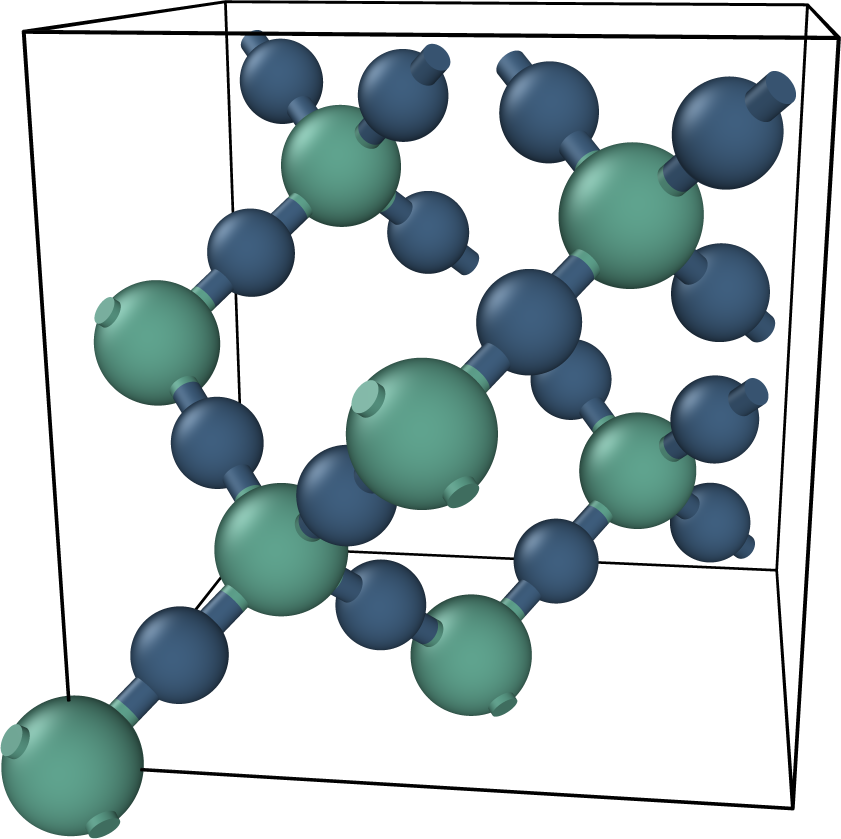
\includegraphics[width=0.6\linewidth]{figures/unitcell/unitcell.png}
	\caption{Unit cell of b-cristobalite. Tan and blue spheres represent silicon and oxygen atoms respectively. The unit cell is cubical, with edges of length 7.12Å.}
	\label{fig:unitcellbcristobalite}
\end{figure}



\section{Building a crystal}
The coordinates gotten from the \texttt{.cif}-file can now be implemented into \textit{moltemplate} together with whatever bond and angle data required by the potential. In our simulations we will use the Vashishta potential, which does not require these. 
Moltemplate has its own structure and syntax. 
The first step to build up a larger material is, as mentioned, to create the unit cell. 
Data concerning the unit cell are placed in a \texttt{.lt}-file, which is readable by Moltemplate. 
Such a file is shown in Listing \ref{lst:beta-cristobalite.lt}. 
For a more profound understanding of the structure and syntax of these files, the reader is advised to read the moltemplate manual\footnote{\url{http://www.moltemplate.org/doc/moltemplate_manual.pdf}}.


\lstinputlisting[caption={Typical Moltemplate file containing unit cell data. The columns of the "Data Atoms" section hold, from left to right, information of atom ID, atom type, x-, y- and z-position. The "Data Masses" section stores the weight of silicon and oxygen atoms in atomic mass units.}, label=lst:beta-cristobalite.lt, language=LammpsData]{../SiO2/large/beta-cristobalite.lt}
We use the unit cells as building blocks, placing them concurrently until we have a crystal of the desired size. For example purposes, we generate a large cube of $15\times15\times15$ unit cells, i.e. 81000 atoms. This is done in line 17-21 of listing \ref{lst:cubeSiO2} below.
\lstinputlisting[caption={Moltemplate script to build a cube out of $15^3$ unitcells of $\beta$-cristobalite (81000 atoms), and also specify system configurations (see section \ref{sec:systemConfigurations}). The "write\_once" sections create the files containing their contents. Line 17 imports the unit cell shown in listing \ref{lst:beta-cristobalite.lt}, and line 19-21 copies it concurrently in a $15\times15\times15$ cube.}, label=lst:cubeSiO2, language=LammpsData]{../SiO2/large/system.lt.latex}
%{\Huge Uncomment the above listing!}
The \textit{write\_once} sections with "In" as the first word of its argument, creates the files \texttt{system.in.init} and \texttt{system.in.settings}, which contain exactly what is shown in the snippet. 
They are not necessary, but help making the LAMMPS input script cleaner, since we can \texttt{import} these files instead of having all the configurations in the input script file.
The last \textit{write\_once} section with "Data" in its argument, incorporates the specified size of the simulation box in the \texttt{system.data} file. 
Line 19 creates a new unit cell at every point separated by 7.12\AA ~in all three dimensions. The positions, and other properties defined by the \textit{atomstyle}, of all the distributed atoms are stored in the file \texttt{system.data} as well. 

The Moltemplate script can be run from the command line as
 \begin{lstlisting}
 moltemplate -atomstyle "atomic" system.lt
 \end{lstlisting}
Once complete, we can load the configurations and atomic data into our LAMMPS input script simply by including the file \texttt{system.in}.



\begin{figure}[H]
	\centering
	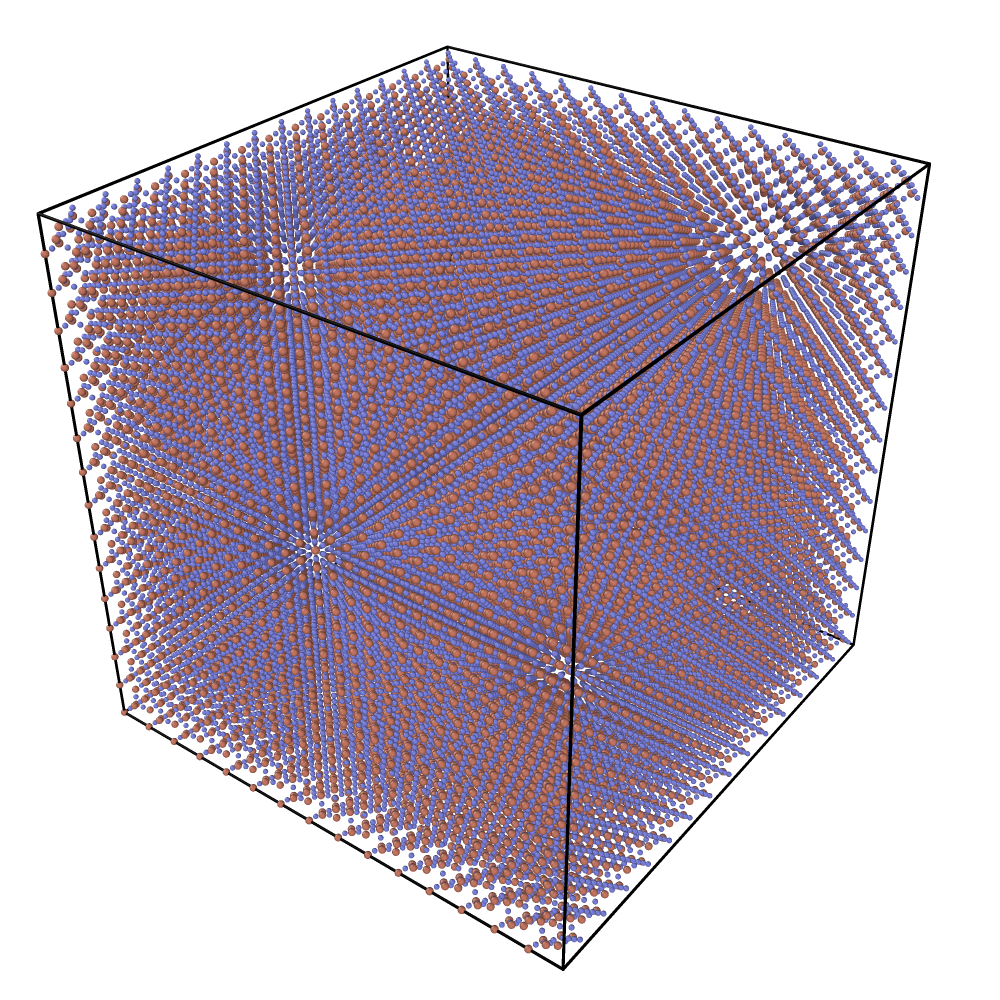
\includegraphics[width=0.7\linewidth]{figures/CreatingSystem/hugeCube}
	\caption{System built from $15\times15\times15$ unit cells of b-cristobalite.}
	\label{fig:hugeCube}
\end{figure}


\section{Melting point}
A simple verification we can do is to estimate the melting point of the material we are using. 
There are several factors that may affect the result, such as density, structure and of course parameters in the potential model. 
When increasing the temperature of the system that is in a solid state, we will eventually reach the melting point.
At the phase transition from a solid state to a liquid, the atoms of the silica will have energy great enough to break the interatomic bonds. 
They will break loose from their regular arrangement and move about much more freely. 
An approach to computing the melting point is therefore to systematically increase the temperature stepwise and sample the mean square displacement of the atoms at each temperature level.  
The mean square displacement is the average of the square of the displacement every atom has from its initial position. It can be expressed as:
\begin{equation}
\langle r^2(t)\rangle = \frac{1}{N}\sum_{i=1}^{N}\lr{\vec{r}_i(t)-\vec{r}_i(0)}^2. \label{eq: diffusion constant}
\end{equation}
where $\vec{r}_i(t)$ is the position of atom $i$ at time $t$ and $N$ is the total number of atoms. 

The mean square displacement is expected to related to the diffusion of atoms though
\begin{equation}
	D = \frac{\langle r^2(t)\rangle}{2dt},
\end{equation}
where $D$ is the diffusion coefficient, and $d$ is the number of dimensions \cite{EinsteinBrowninanMotion}. 

In practice the mean square displacement was computed using a standard \textit{compute} in LAMMPS, namely the \textit{msd compute}\footnote{\url{http://lammps.sandia.gov/doc/compute_msd.html}}. 
At every time step it stores a vector of 4 elements; the first 3 are the squared $dx$, $dy$ and $dz$ displacements averaged over the atoms of the specific group, while the 4th is the total mean square displacement for the specific group, i.e. $(dx^2 + dy^2 + dz^2)$. 
The $15\times15\times15$ system is sufficient for this test. The procedure is rather simple. For $\beta$-cristobalite we expect the melting point to be about 1986K\footnote{\url{https://en.wikipedia.org/wiki/Cristobalite}}, so we start out at 1500K. After equilibration the following steps are repeated until we reach a target temperature. 
\begin{itemize}
	\item equilibrate for the current temperature
	\item compute msd for $N$ time steps
	\item increase the temperature by a given step size
\end{itemize}
\lstinputlisting[caption={Section of LAMMPS script illustration how to stepwise increase temperature and compute the mean square displacement of atoms.}, label={lst:msd}, firstline=14, lastline=40]{../SiO2/msd/continue.in}
\begin{figure}[H]
\centering
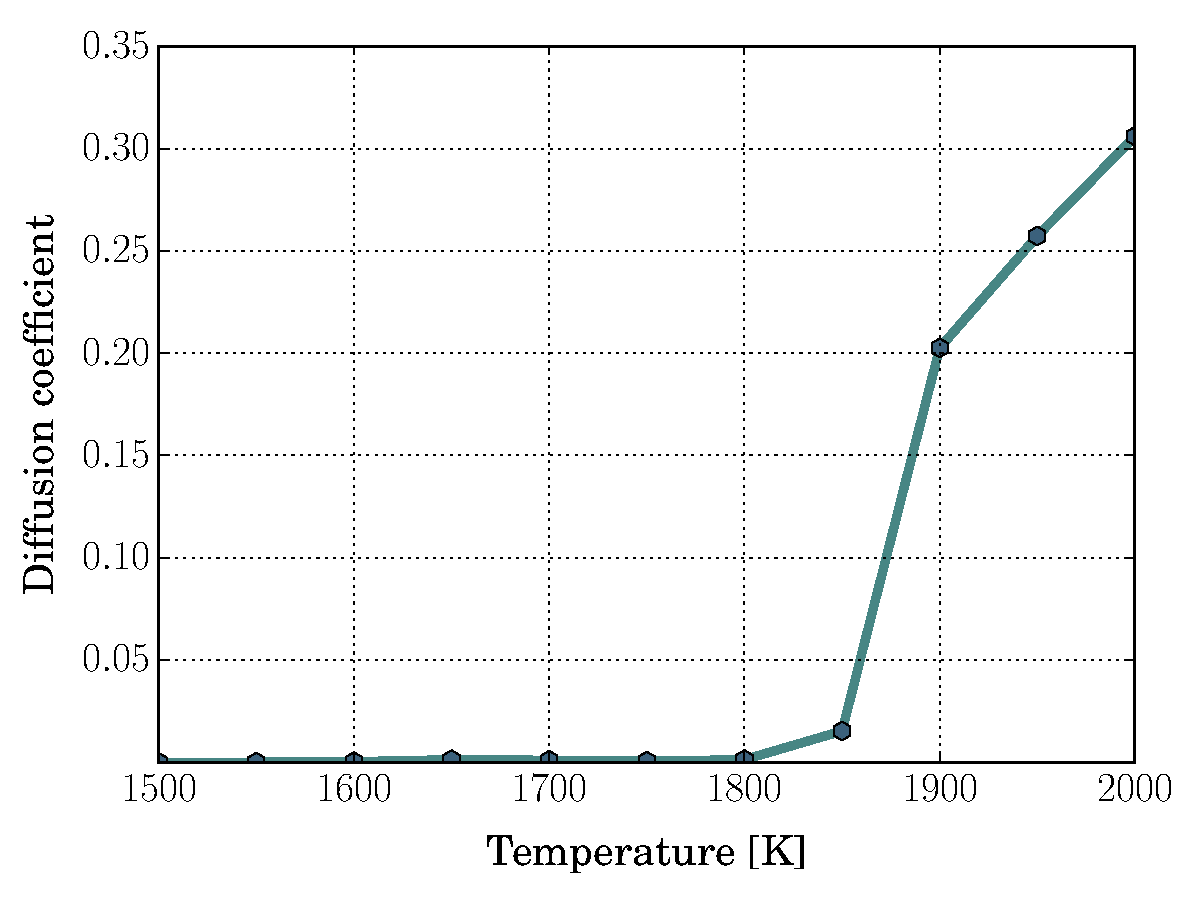
\includegraphics[width=0.7\linewidth]{../SiO2/msd/figures/msd}
\caption{Measured diffusion coefficient as a function of increasing temperature. 
	The face transition occurs where we see a rapid change in the behavior. 
	Here we can estimate the measurement somewhere between 1850K and 1900K. 
	These measurements were obtained from a cubical simulation box containing $15^3$ unit cells of $\beta$-cristobalite (81000 atoms) evenly distributed, and with periodic boundary conditions.}
\label{fig:msd}
\end{figure}
This result infer a melting point somewhere in the range 1800K-1900K. 
Believe it or not, this is actually a pass on the test! 
In fact, anything deviating less than $20\%$ from the experimental results is considered a pass, as stated by the developers of the potential. 
Unfortunately, this also show that there are some qualitative detail that is lost, and that when using this potential we should probably focus on the quantitative behavior. 





\section{Shaping the system}

%\begin{figure}
%	\centering
%	
\includegraphics[width=0.7\linewidth]{figures/CreatingSystem/drawing.pdf}
%	\caption{Illustrative drawing of what how the system should look. Red parallel stripes symbolize areas of silica. Red crossing stripes indicate areas of frozen silica. The boundaries are periodic in all dimensions, causing both the slab and the sphere to be connected to the frozen silica through the z-boundaries.}
%	\label{fig:drawing}
%\end{figure}

The huge cube of silica can be carved however we like by defining regions from which we delete the containing atoms. 
In LAMMPS this is done using the \texttt{region}, \texttt{union}, \texttt{intersect} and \texttt{delete\_atoms} commands. 
Our implementation is stated in Listing \ref{lst:sculpting}, which is very simple due to the way we are going to treat the boundary conditions. 
We start out by defining a spherical region labeled \texttt{sphereRegion}, described by the xyz-coordinates of its center and a radii. 
The atoms within this region are assigned to a group labeled \texttt{sphereGroup}. 
Next, we define a cuboid (block) region named \texttt{slabRegion}, described by the position of its faces in x-, y- and z-direction. 
The atoms within this region are assigned to a group, which we label \texttt{slabGroup}.  
We combine these two regions using  the \texttt{union} command and label the region outside of these regions \texttt{outRegion}.
Finally, we delete the atoms that are not in the sphere nor the slab; we delete the ones contained by \texttt{outRegion}.
\lstinputlisting[caption={Defining regions to keep or delete from a system of dimensions $106.8\times106.8\times106.8$ Å.}, label={lst:sculpting}]{../SiO2/small/system.prepare.latex}
For the purpose of deleting atoms, the creation of groups was superfluous.
However, at a later stage we will utilize them and this is an appropriate place for them to be assigned. 
The appliance of the script in Listing \ref{lst:sculpting} on the system is shown in figure \ref{fig:hugeCube} is shown in figure \ref{fig:carvedxz}, where our perspective is along the y-axis.
\begin{figure}[H]
\centering
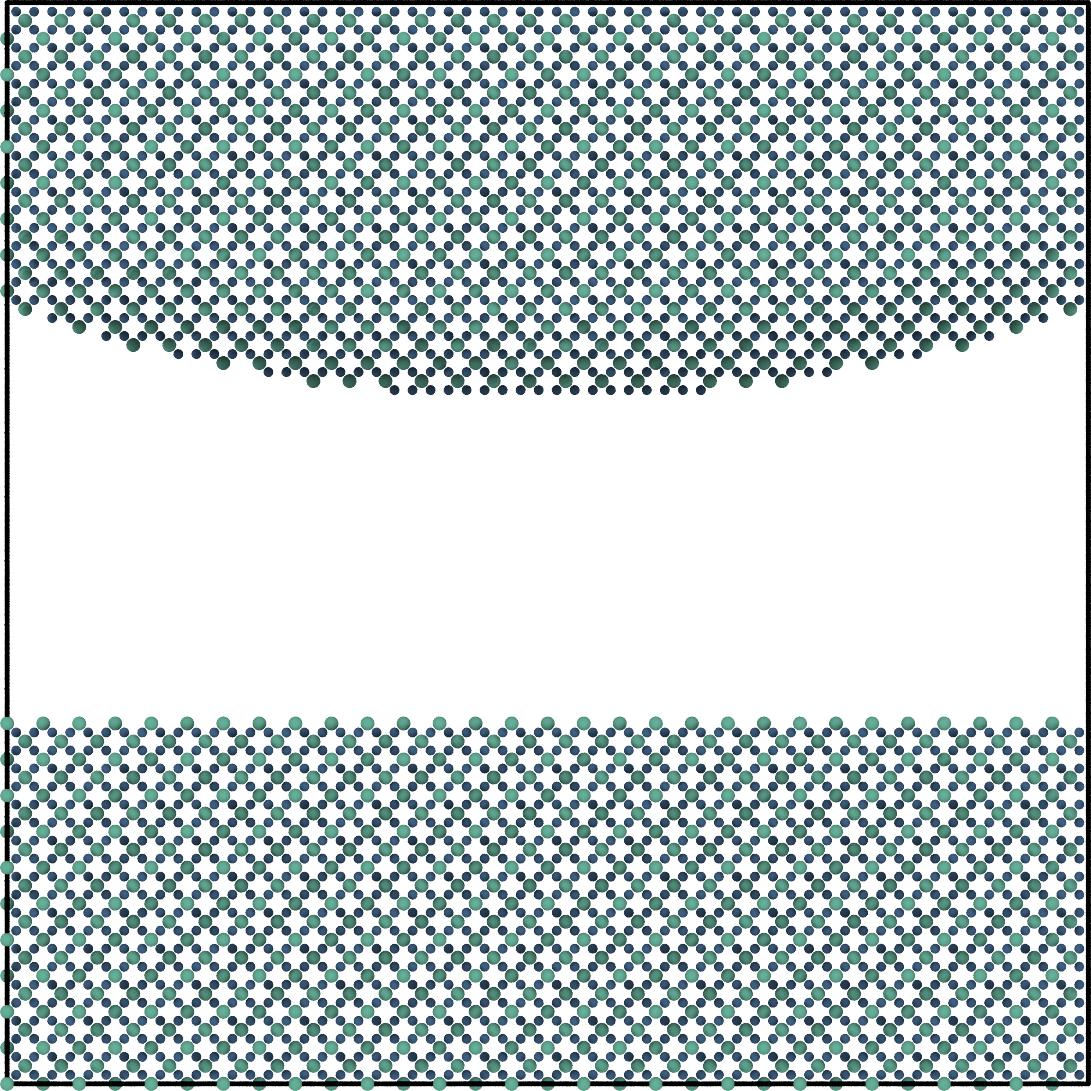
\includegraphics[width=0.5\linewidth]{figures/CreatingSystem/carved_xz.png}
\caption{xz-perspective on a system built from $15\times15\times15$ unit cells of b-cristobalite, with certain regions carves out. This is a result from applying Listing \ref{lst:sculpting} to the system shown in figure \ref{fig:hugeCube}. The top shape is a sphere cap, while the bottom is a slab.}
\label{fig:carvedxz}
\end{figure}


\section{Moving the sphere towards the slab}
We wish to push the sphere down onto the slab in order to create a deformation on the slab. There are many approaches to accomplish this. 
One could apply an external force, pushing the sphere with a controlled force. 
Another is to move the sphere at a controlled, constant velocity.  
We will use both of these methods on separate parts of the project.
For the first part, we have settled on the following strategy:
We apply periodic boundary conditions in all three dimensions. 
%This will in practice imply that the sphere cap and the slab are connected through the z-boundaries. 
Secondly, we freeze the atoms at the bottom of the slab so that their positions are fixed. 
They still interact with other atoms, but we restrain them from moving. 
This will, due to the periodic boundary conditions, allow us to consider the sphere cap and the slab as if they are not connected to each other, but to independent blocks of silica glass.  
For every $N$ time steps we decrease the height of the system, while remapping the positions of the atoms. 
The remapping is a very important procedure. 
It ensures that we do not lose any atoms that else-wise would be lost when moving the z-boundary. 
A side-effect of the remapping is that the atoms in the system will be somewhat compressed in the z-direction. 
Though, if we do the compression slowly, this will not be of any concern. 

One technique to fix atom positions is to explicitly set their velocity and force to zero at every single time step.
A more efficient method is to simply omit the atoms of consideration from time-integration. 
This way we do not bother computing the force acting on them, updating their velocity or position at all! 
To do this, we simply create a group that contains all atoms except the once who should be fixed.
Listing \ref{lst:FreezeStuff} show how to tell LAMMPS to only time-integrate the atoms in the group \texttt{excludingBT}, which excludes the bottom and tom regions of our system.
The omitted atoms are still considered to be present, we just don't bother updating their movement.

To deform/resize the system, we may use the command shown in listing \ref{lst:Deform}. 
This command changes the position of the upper boundary of in the z-dimension, by the length \texttt{compressionLength} during a \texttt{run}.
Thus if we choose the run to last $N$ time steps, the boundary will move with the velocity 
\begin{equation}
	\vec{v}_z = -\frac{\texttt{compressionLength}}{N\cdot0.002} ~~ [\text{\AA/ps}]
\end{equation}
since our time steps are $0.002$ ps.
\begin{lstlisting}[caption={Time-integrating only atoms in a specified group, \texttt{excludeBT}, effectively fixing all others.}, label={lst:FreezeStuff}, language=LammpsInput]
fix nvtID excludeBT nvt temp ${T} ${T} 1.0
\end{lstlisting}

\begin{lstlisting}[caption={LAMMPS command for deforming the simulation box, and remaping atom positions.}, label={lst:Deform}, language=LammpsInput]
fix ID all deform 1 z delta 0 -${compressionLength} remap x
\end{lstlisting}
 

\begin{comment}
\chapter{This must be sorted in designated chapters}

\section{Radial distribution of normal force}
In order to find a radial distribution of the normal force, $F_N$, we partition the system into a grid in  the xy-plane. We then use the command 

\begin{lstlisting}[language=LammpsInput]
	compute chunkID all chunk/atom bin/2d x 0 7.12 y 0 7.12
	compute stressID all stress/atom NULL
	fix fixChunkID all ave/chunk 1 1 10 chunkID c_stressID[3] file forcesInChunks.txt
\end{lstlisting} 
to compute the stress of every chunk in the z-direction, $\sigma_{zz}$ (sum of every individual atom stress in the chunk). 

Line 1 establishes the grid, with bin width $7.12$Å.

Line 2 creates a compute of the stress

Line 3 stores the sum of individual stresses in each chunk to the file \texttt{forcesInChunks.txt}. 
This is done every 10 time steps in order to reduce correlation effects. 

The data in stored from each time step can easily be averaged to produce a result as shown in figure X.

We can then find the radial distribution simply by binning this matrix in radial bins, and average the normal forces of the chunks within the bins.

\end{comment}





\part{Numerical simulations and results}

\chapter{Computing contact forces}
Contact forces are forces acting between two bodies at the area of contact. 
They can be decomposed into normal an shear forces 
The normal force is defined as the force exerted on an object that is perpendicular to the contact surface, while shear force is the component lying tangential to the contact surface.
%The system we have created will have a non-zero normal force in the indentation of the substrate. 
In this chapter we will make an attempt to find the distribution of the normal and shear forces acting between a spherical cap indenting a substrate. 
This is not a trivial thing to compute in molecular dynamics. 
The reason is that we have to be able to define the contact surface, which is not always easy. 
For solid state physics there are several algorithms which attempt to do this by searching for areas with structural discrepancies or dislocations \cite{stukowski}. 
As time was a limiting factor, a simpler approach has been used. 
Secondly, we must distinguish contact forces from non-contact forces. 
As a matter of fact, to obtain the contact forces we have expanded the LAMMPS library by creating a custom compute class, since there currently is no such compute available. 
For the sake of completeness, the details of that procedure will be described.

Our strategy is simple, but not necessarily easy. 
First of, we divide the system into a 2D-grid in the xy-plane. 
Secondly,  we compute the time-averaged force exerted on one body from another within the region of each cell in the grid. 
We approximate the slope of the contact surface within the cells using a least squares regression method on the atoms positioned at the surface. 
Finally, we project the average force of a cell onto the corresponding normal vector of the approximated surface.

The results will be posed graphically at the end of the chapter, as 3-dimensional plots in polar coordinates, with the corresponding radial distribution. 


\section{Creating a custom compute}
A \textit{compute} is a LAMMPS command that defines a computation that will be performed on a group of atoms. 
The \textit{computes} produce instantaneous values, using information about the atoms on the current time step\footnote{\href{ http://lammps.sandia.gov/doc/compute.html}{ http://lammps.sandia.gov/doc/compute.html}}.
In LAMMPS there are more than 100 computes and chances are, they already have what you're looking for. If not, one might treat the data from other computes in some way to get the desired information. However, if there are no compute command that does the desired task, it is possible to create an own custom class and thereby expanding the LAMMPS library.  
In order to compute the normal forces acting on the sphere, we have written a custom compute class. 
The objective was for the class to save the force acting on each atom in one group from atoms of another group. 
In this section we will try to give a brief summary on how this was done.


\subsection{Look for similar computes}
Obviously, before writing any code we should know what we want the compute to calculate and how this should be done. 
Before starting off with a blank sheet in the editor, one should definitely search for similar computes in LAMMPS. This can potentially save hours of hard work!
Our case serves as a good example.
There is a compute named \textit{group/group}\footnote{\href{http://lammps.sandia.gov/doc/compute_group_group.html}{http://lammps.sandia.gov/doc/compute\_group\_group.html}} which computes the total energy and force interaction between two groups of atoms. 
This is almost what we want, but we need to know the force acting on each atom from atoms of other groups. 
Also, It should work with the Vashishta potential, which \textit{group/group} currently does not.
Thus, there are minor modifications needed and because of the similarities we chose to make our compute a subclass of this one.


\subsection{Creating the class}
All computes in LAMMPS are subclasses of the class named  \textit{compute}. 
From this superclass they inherit a bunch of variables, functions and flags, which the user may decide to set. 
Functions are of course declared in the header file, while variables and flags are set in the source file. 
The source code of the \textit{group/group} compute is included in the LAMMPS distribution. 
Since we will be making a subclass of it, we change the \textit{private} property to \textit{protected} so that we have access to all the variables and functions, from our subclass.

We start out by creating a header file and decide upon a name for our class. 
We have chosen the name \textit{group/group/atom} since it is basically a per-atom version of the already existing compute \textit{group/group}. 
A trailing {\it "/atom"} is the common naming convention of per-atom computes. 
A complete header-file is shown in Listing \ref{groupGroupAtomHeader} and explained in detail below.

\lstinputlisting[caption={Header file of our new compute: \texttt{compute\_group\_group\_atom.h}.}, label={groupGroupAtomHeader}, language=c++, firstline=14, lastline=40]{../../LAMMPS/src/compute_group_group_atom.h}
As can be seen, there are not many additions to the variables and functions already existing in the superclass, as the main difference lies in the structure we store the computed values.

\begin{itemize}
\item \texttt{ComputeStyle} defines the command to be used in the input script to be \linebreak[1] \texttt{group/group/atom}, and the name to be \texttt{ComputeGroupGroupAtom}. 
	The name is of no importance though. 
\item \texttt{nmax} is the number of atoms which are subject to a non zero force from atoms of another group at the current time step; it may vary.

\item \texttt{carray} is a two dimensional array containing the force on atoms in one group induced by atoms of another group. Its dimension will necessarily be \texttt{nmax} $\times$ 3.

\item \texttt{compute\_peratom()} and \texttt{pair\_contribution()} are functions which will be described below the corresponding source file. 
\end{itemize}


\lstinputlisting[caption={Source file of compute: \texttt{compute\_group\_group\_atom.cpp}.}, label={lst:groupGroupAtomSource}, language=c++, firstline=19, lastline=300]{../../LAMMPS/src/compute_group_group_atom.cpp}

\subsubsection{Setting flags}
In the constructor we set specific flags that LAMMPS uses to interpret what structure our data should have, and how to store them. 
We set the \texttt{peratom\_flag} to be \texttt{True}, which indicates that we desire to store some data for each atom. 
\texttt{size\_peratom\_cols} defines the number of data values to store for each atom. 
The flag \texttt{extarray} is set to \texttt{False}, indicating that the per-atom value is an intensive value. 
Also, we set the \texttt{scalar\_flag} and \texttt{vector\_flag} to \texttt{False}, since we do not wish to return a vector or scalar value.

\subsubsection{Destructor}
Following the constructor is the destructor on line 40. Its only task is to free the memory occupied by the array once it is no longer needed.  

\subsubsection{compute\_peratom()}
 If necessary, this function will resize the array to the number of atoms of concern, \texttt{nmax}. 
 It does this using internal functions in the superclass \textit{compute}, which we will not care to describe here. 
 Finally it calls upon the function \texttt{pair\_contribution()}, which fills the per-atom arrays with the energy and force components. 
 A very important detail is that we only use the pair-contribution of the potential. 
 We only sample the two-body part of the energy and force components. 
The many-body corrections are ignored.
Hence, our measurements will lack that detail.
Nevertheless, the two-body term is by far the predominant portion of the potential, and our results should be quantitatively correct.  

\subsubsection{pair\_contribution()}
In this function we sample the two-body force acting on each atom of a group from all atoms of another group. 
Before we dive into the code, some of the variables are described.

\begin{itemize}
\item[] \texttt{inum} is the number of atoms (assigned to the processor).

\item[] \texttt{ilist} is a list of the atom indices of the atoms contained by the processor.

\item[] \texttt{numneigh} is a list of the number of neighbors each atom has.

\item[] \texttt{firstneigh} is the actual neighbor list. Thus, a 2-dimensional list containing the index of each neighbor for each atom.

\item[] \texttt{groupbit} is a 32-bit integer associated with a specific group. 

\item[] \texttt{mask[i]} is a 32-bit integer containing information on which groups atom \texttt{i} is part of.  
\end{itemize}

On line 93 we loop over all atoms (assigned to the processor), and assign the atom index to the variable \texttt{i}, on the next line. 
We then explicitly set their energy and force entries to zero. 
%This is necessary because LAMMPS may rearrange the list holding atom indices, \texttt{ilist}, causing each individual computation to be correct, but in post processing?
Line 102 - we loop through all atoms again, to fill these entries. 
First, we check if atom \texttt{i} is in the compute group or the second group, by doing a bitwise comparison of the atoms group-int with the group-bits. If it's not, we end the iteration and continue to the next atom.
Line 109 - We store the position and type of atom \texttt{i}.
Line 118 - Loop through all neighbors \texttt{j} of atom \texttt{i}.
Line 120 - 121 - Special stuff!
Line 125 - Check if \texttt{j} is in either of the groups
Line 128 - Sort out which group \texttt{i} and \texttt{j} are part of. 
If they are in the same group, we end the current iteration and continue to the next.
Line 137 - Compute the square distance between the two atoms.
Line 145 - If the interdistance is shorter than the cutoff length, compute the potential energy and interaction force. 
The force is normalized by the displacement,  so that $\texttt{fpair}=F_{ij}/r_{ij}$.
Line 151 - We sample the energy and force components in the per-atom array. 
If we do not use newtons third law, we sample the energy contribution twice inside \texttt{pair->single}. Hence, we must half the contributions in that case.


\subsection{Usage}

%The arrays returned are not ordered in any way. 
%This is not a cause of concern to us, though.
%We are simply interested in knowing the position, and value of the force components of each atom. 
 \begin{lstlisting}[language=LammpsInput, caption={Syntax for using custom compute}, label={lst:customComputeSyntax} ]
	compute ID group1-ID group/group/atom group2-ID keyword value
\end{lstlisting}
The compute class shown in listing \ref{lst:groupGroupAtomSource} calculates the energy and force interaction between each atom in group1 and all atoms in group2. The groups can be the same group. It is invoked by using the syntax in listing \ref{lst:customComputeSyntax},
where \\*
\begin{itemize}
	\item ID is the reference to the invoked compute.
	\item group1-ID and group2-ID are the specified groups we wish to compute the energy and interaction force between. The energy and interaction force is only stored for atoms in group1, and the force is the force acting on group1 from group2.
	\item keyword is optional and can be either \textit{pair}, \textit{kspace}, \textit{boundary} or \textit{molecule}, with value \textit{yes} or \textit{no}. For a description of these, please look up the documentation for compute group/group\footnote{\href{http://lammps.sandia.gov/doc/compute_group_group.html}{\url{http://lammps.sandia.gov/doc/compute_group_group.html}}}. 
\end{itemize}
The compute successfully stores the contact force components of all atoms in an array when invoked. 
We are interested in the spatial distribution of the forces. 
To obtain it, we divide the system into a 2d-grid in the xy-plane, using  \texttt{compute chunk/atom} as shown in listing \ref{lst:usingCustomCompute}.
On the next line we call upon our compute, stating that we wish the force acting on the sphere from the slab. 
Thus, the force that should have a positive z-component in this case. 
We could be content with using the result from a single time frame, but since the instantaneous values fluctuate, it's of interest to apply time averaging. 
The \texttt{compute ave/chunk} is used for summation and time averaging.  
It sums the  per-atom vectors of atoms in each chunk from specified time steps, and averages this over time. 
We obtain a matrix of the time-averaged value of the sum of force components on atoms within each grid element of the system.
This is stored to a text-file with specified name. 

At this point, we can study for instance the distribution of the magnitude of contact force, or contact force in a specified direction as in figure \ref{fig:forceDistributions} .
%Notice how some of the grid elements have a negative z-component in figure \ref{fig:zForceDistribution}.
The speckles outside the contact area are atoms/molecules that have broken loose from their original bonds, and drifted until they attached to the other body. 
In retrospect, it is obvious that this could be avoided by redefining the groups after the equilibration procedure.
Though, as it will not alter the quantitative results, this was ignored.


 \begin{lstlisting}[language=LammpsInput, caption={Example usage of compute group/group/atom with spatial binning and time averaging.}, label={lst:usingCustomCompute} ]
compute chunkID all chunk/atom bin/2d x 0 7.12 y 0 7.12
compute ggaID sphereG group/group/atom slabG pair yes
fix fixComputeID sphereG ave/chunk ${Nevery} ${Nrepeat} ${Nfreq} chunkID c_ggaID[2] c_ggaID[3] c_ggaID[4] file forces.txt
\end{lstlisting}

\begin{figure}[H]
	\centering
	\begin{subfigure}{0.49\textwidth}
		\centering
		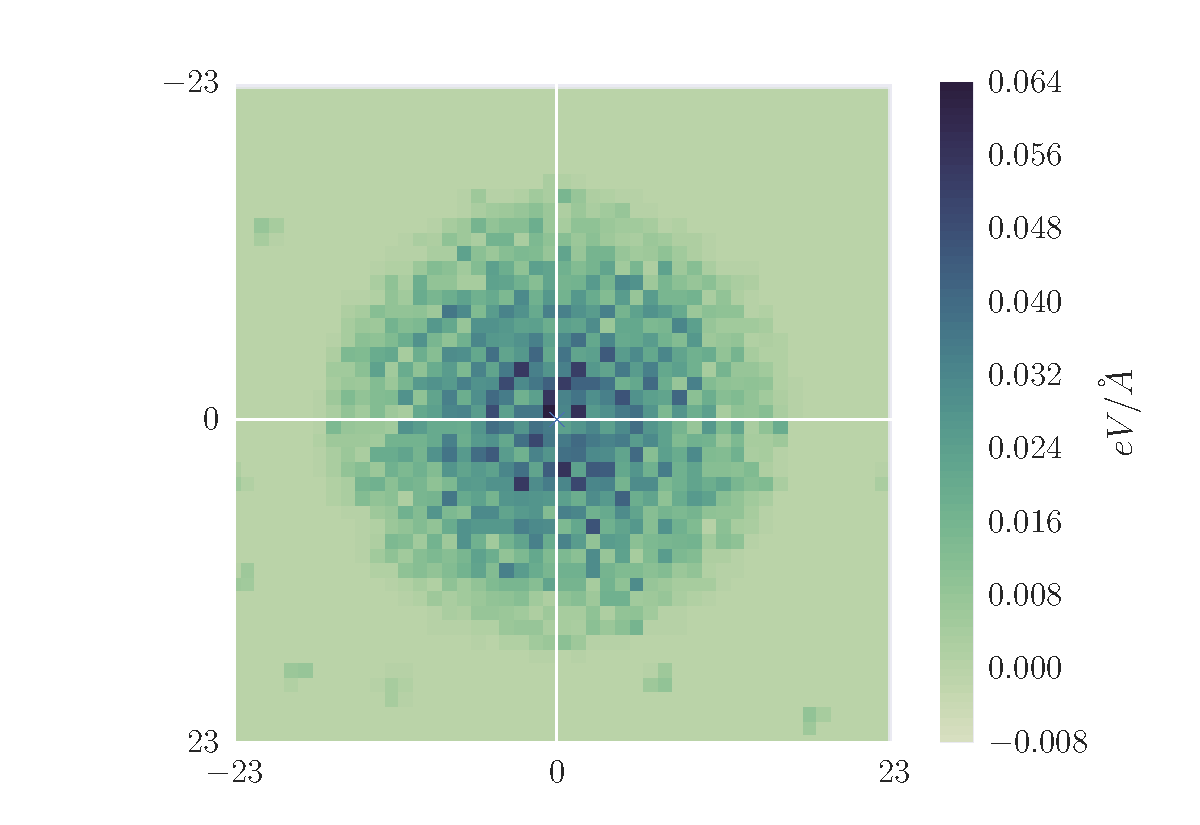
\includegraphics[width=\linewidth,  trim={15mm 2mm 7mm 2mm}, clip]{figures/forceDistribution/forces/absoluteForceDistribution.pdf}
		\vspace{-7mm}
		\caption{Magnitude of force.}
		\label{fig:absoluteDistribution}
	\end{subfigure}
	\begin{subfigure}{0.49\textwidth}
		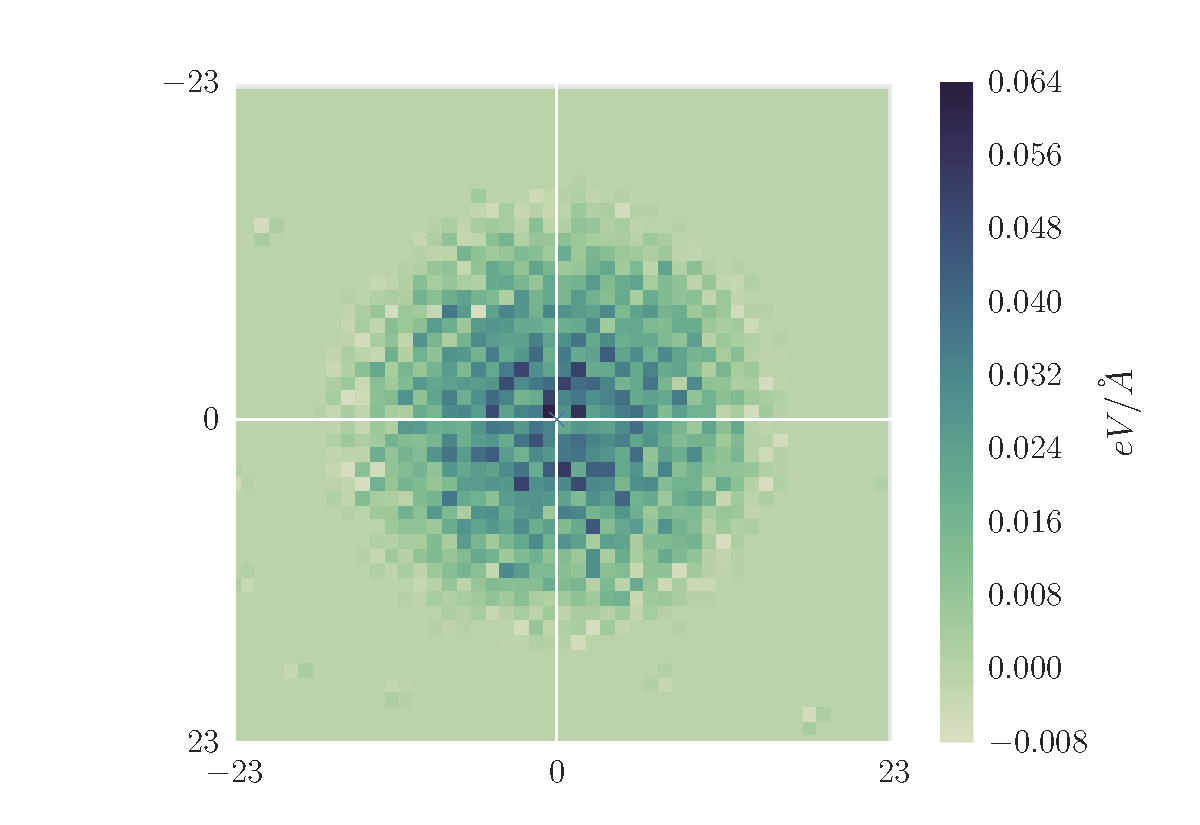
\includegraphics[width=\linewidth, trim={13mm 2mm 9mm 2mm}, clip]{figures/forceDistribution/forces/zForceDistribution.pdf}
		\vspace{-7mm}
		\caption{Force in z-direction.}
		\label{fig:zForceDistribution}
	\end{subfigure}
	\vspace*{5mm}
	\caption{Distribution of force. The color at a square represents the time averaged magnitude (a) and z-component (b) of the contact force of atoms within the square, hence not dependent on direction.
		This is the result from a simulation where we push a sphere with radius of curvature $R=200\mathring{A}$, $40\mathring{A}$ into a half-space of area $46\times46$ unit cells}
	\label{fig:forceDistributions}
\end{figure}

\newpage
\section{Least squares plane regression} \label{sec:leastSquareRegression}
The method of least squares aims to find parameters which  minimize the sum of the squared residuals, where residuals are the difference between observed values and the approximated value. We will use this method to approximate the slope of the surface of the substrate. This will be done by partitioning the system in a grid and do a plane approximation on each cell of the grid. In other words, we seek the coefficients in the plane equation
\begin{equation}
	z = ax + by + c
	\label{planeEquation}
\end{equation}
that minimizes the sum of the squared residuals
\begin{equation}
	S = \sum_{i=1}^{n} r_i^2 = \sum_{i=1}^{n} \lr{z_i - f(x_i, y_i, \vec{\beta)}}^2,
	\label{leastSquaresPlane}
\end{equation}
where $f(x_i,y_i,\vec{\beta})$ is the right hand side of the plane equation and $\vec{\beta}$ is the set of coefficients.
The minima has the property that the differential with respect to any coefficient is zero. 
\begin{equation}
	\frac{\partial S}{\partial \beta_j} 
	=  \sum_{i=1}^{n}\frac{\partial r_i^2}{\partial \beta_j} 
	=  \sum_{i=1}^{n}\frac{\partial r_i^2}{\partial r_i} \frac{\partial r_i}{\partial \beta_j} 
	= -2 \sum_{i=1}^{n}r_i\frac{\partial f(x_i,y_i, \vec{\beta})}{\partial \beta_j}
	= 0 , ~\forall ~\beta_j \in \vec{\beta}
\end{equation}
When approximating a plane we have three coefficients to account for: $a$, $b$ and $c$. This leaves us with the following set of equations:

\begin{align}
	&-2 \sum_{i=1}^{n} \lr{z_i - ax_i - by_i- c} \frac{\partial}{\partial a} \lr{ax_i + by_i + c} = 0 \\
	&-2 \sum_{i=1}^{n} \lr{z_i - ax_i - by_i- c} \frac{\partial}{\partial b} \lr{ax_i + by_i + c} = 0 \\
	&-2 \sum_{i=1}^{n} \lr{z_i - ax_i - by_i- c} \frac{\partial}{\partial c} \lr{ax_i + by_i + c} = 0,
\end{align}
 which corresponds to
 \begin{align}
 \hspace{25mm}&\sum_{i=1}^{n} z_ix_i& &=& &a\sum_{i=1}^{n} x_i^2& &+& &b\sum_{i=1}^{n} x_iy_i& &+& &c\sum_{i=1}^{n} x_i \hspace{15mm}\\
 &\sum_{i=1}^{n} z_iy_i& &=& &a\sum_{i=1}^{n} x_iy_i& &+& &b\sum_{i=1}^{n} y_i^2& &+& &c\sum_{i=1}^{n} y_i \\
 &\sum_{i=1}^{n} z_i& &=& &a\sum_{i=1}^{n} x_i& &+& &b\sum_{i=1}^{n} y_i& &+& &nc . 
 \end{align}
This can be expressed as a matrix equation.

\begin{equation}
\left[ \begin{array}{llc}
\displaystyle \sum x_i^2  &\displaystyle \sum x_iy_i &\displaystyle \sum x_i \\[1em]
\displaystyle \sum x_iy_i &\displaystyle \sum y_i^2  &\displaystyle \sum y_i \\[1em]
\displaystyle \sum x _i   &\displaystyle \sum y_i    &\displaystyle n
\end{array} \right]
\left[ \begin{array}{c}
\vspace{1mm}a\\[1em]
\vspace{1mm}b\\[1em]
\vspace{0.5mm}c
\end{array} \right]
=
\left[ \begin{array}{l}
\displaystyle \sum x_iz_i \\[1em] 
\displaystyle \sum y_iz_i \\[1em]
\displaystyle \sum z_i
\end{array} \right]
\label{linearSystemPlane}
\end{equation}
where we have omitted the indices to better readability.
Solving this linear system retrieves the optimal coefficients in the sense of the least squares method. 
The normal vector of the plane will be $\vec{n}=[a,b,1]$. 
This vector will be used to compute the size of the normal force. 
Since we know the average force on an atom in the chunk, and the normal vector from the approximated slope of the surface, we can compute the normal force simply as

\begin{equation}
	\vec{F_N} 
	= |\vec{F}|\cos{\theta}\frac{\vec{n}}{|\vec{n}|} .
\end{equation}
The cosine of the angle between the two vectors is given as
\begin{equation}
	\cos{\theta} = \frac{\vec{F}\cdot\vec{n}}{|\vec{F}| \cdot |\vec{n}|},
\end{equation} 
meaning that the normal force may be expressed as
\begin{equation} 
%	\vec{F_N} = \frac{\lr{\vec{F}\cdot\vec{n}}}{|\vec{n}|} \frac{\vec{n}}{|\vec{n}|} .\\
\vec{F_N} = \lr{\vec{F}\cdot\vec{n}} \frac{\vec{n}}{|\vec{n}|^2} .
\end{equation}
In general there are two valid normal vectors $\vec{n}$ that satisfy the plane equation. However, this procedure assures that we always get the one with a positive z-component.  
If we compute the contact forces acting on the sphere from the substrate, a positive normal force, will imply a repulsive force, while a negative value an attractive force.

%{\color{editColor} We will assume that the normal vector $\vec{n}$ is always in the same general direction as the average force, though obviously it may just as well point in the opposite direction and still be a normal vector to the plane. Programatically this was done in python as shown in \ref{angleVecLine}.} 

%\lstinputlisting[caption={Python function to compute the smallest angle between a vector and a line parallel to another vector. }, label={angleVecLine}, language=python, firstline=190, lastline=197]{../SiO2/large/pythonScripts/surface.py}

\newpage


\section{Radial distribution}
Our system is partitioned into a grid. 
Each cell in the grid holds an averaged value of the normal force in that cell. 
We would like to know the radial distribution of the normal force, which should express the averaged value of the normal force at a given radial distance from the center of the spherical indentation.
We achieve this by defining discrete radial bins with finite bin width, and average contributions within each bin.
\begin{figure}
	%\begin{minipage}[t]{0.49\linewidth}
	%	\captionsetup{width=\textwidth}
	\centering
	\resizebox{0.4\linewidth}{!}{
		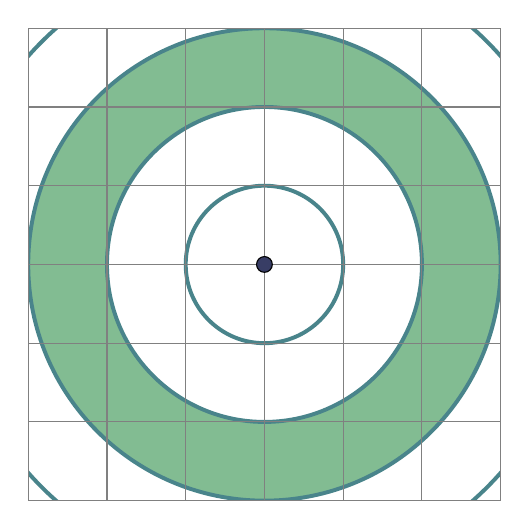
\begin{tikzpicture}
\begin{scope}
\clip (-3,-3) rectangle (3,3);
\draw[p4,line width=0.5mm, fill=p2] (0,0) circle (3cm);
\draw[p4,line width=0.5mm, fill=white] (0,0) circle (2cm);
\draw[p4,line width=0.5mm, fill=white] (0,0) circle (1cm);
\draw[p4,line width=0.5mm] (0,0) circle (4cm);
\end{scope}
\draw[gray] (-3,-3) grid (3,3);
\draw[fill=p6] (0,0) circle (1mm);
%\draw[thick, p6] (1,1) rectangle (2,2);
\end{tikzpicture}
	}
	\caption{Radial binning. The third radial bin is colored, and its value will be the average value of the contribution within the bin.}% A close-up of the outlined cell, is shown in figure \ref{fig:radialBinningSmoothCloseUp}.}
	\label{fig:radialBinningSmooth}
	%\end{minipage}
	%\quad
	%\begin{minipage}[t]{0.49\linewidth}
	%	\captionsetup{width=\textwidth}
	%	\resizebox{\linewidth}{!}{
	%		
\begin{tikzpicture}
\draw[fill=p2] (6,6) rectangle (12,12);
\begin{scope}
\clip (6,6) rectangle (12,12);
\fill[thick, white] (0,0) circle (12);
\draw[thick, p4, line width=3mm] (0,0) circle (12);
\end{scope}
\draw[gray] (6,6) rectangle (12,12);
\end{tikzpicture}
	%	}
	%	\caption{Close-up of outlined cell in figure \ref{fig:radialBinningSmooth}. The contribution from this cell will be it weight multiplied by the fraction of its total area that is colored. I might use this figure to explain the procedure. }
	%	\label{fig:radialBinningSmoothCloseUp}
	%\end{minipage}
\end{figure}
A coarse method of doing this is to average the weights of the cells who's center is within the bin. 
This is illustrated in figure \ref{fig:radialBinningChoars}. 
In many applications where the bin width can be large compared to the length of the cells, this method might suffice.
However, the current radii of the contact area between the sphere and the slab is only about 15-20 unit cells, and therefor having a large bin width will result in very few data points. 


A different, slightly more sophisticated approach is to compute the fraction of the area of each cell that actually is within the bin, and multiply this by the value associated with the cell.
We can sum all these contributions and average them by dividing by the area of the bin. 
This means that even cells that do not have their center within the bin might contribute to the resulting bin value. 
How much, however, will depend on the fraction of the cell's area that is within the bin.
This may be regarded as a smoothing of our coarse force distribution, and will give a more correct result than the coarse binning method already described. 
An illustration of this binning method is shown in figures \ref{fig:radialBinningWeights}.
The figures clearly show that some cells have a larger area within the bin than others, and thus contribute more. 


By exploiting the symmetry we are only required to compute the weights for cells in a section of the domain, and not all cells. 
I have chosen to regard only the upper right corner of the system, meaning $x\geq x_c$ and $y\geq y_c$, where $(x_c, y_c)$ is the coordinates of the center of the indentation.
As the actual computations are easy to follow from the source code, the reader is encouraged to take a look at it if this is of interest. 
In our computations we have regarded unit cell length (7.12\AA) as unit of length.
The bin width was set to 1, though this is allowed to vary. 


\begin{figure}[H]
	\center
	\resizebox{0.4\linewidth}{!}{
		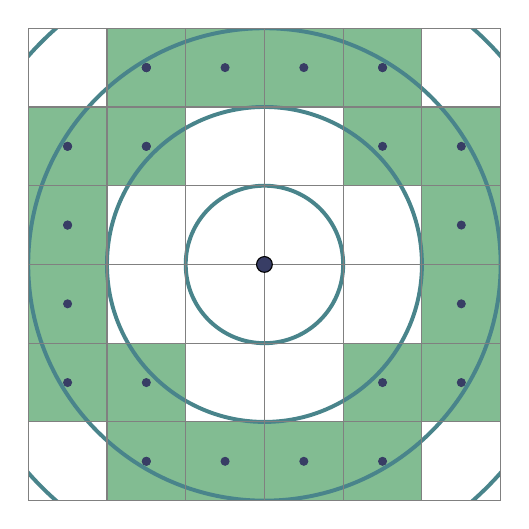
\begin{tikzpicture}
\begin{scope}
\clip (-3,-3) rectangle (3,3);
\draw[gray, fill=p2] (0,2) rectangle (1,3);
\draw[gray, fill=p2] (1,2) rectangle (2,3);
\draw[gray, fill=p2] (1,1) rectangle (2,2);
\draw[gray, fill=p2] (2,1) rectangle (3,2);
\draw[gray, fill=p2] (2,0) rectangle (3,1);

\draw[gray, fill=p2] (0,-2) rectangle (1,-3);
\draw[gray, fill=p2] (1,-2) rectangle (2,-3);
\draw[gray, fill=p2] (1,-1) rectangle (2,-2);
\draw[gray, fill=p2] (2,-1) rectangle (3,-2);
\draw[gray, fill=p2] (2,-0) rectangle (3,-1);

\draw[gray, fill=p2]  (0,-2)  rectangle (-1,-3);
\draw[gray, fill=p2] (-1,-2) rectangle (-2,-3);
\draw[gray, fill=p2] (-1,-1) rectangle (-2,-2);
\draw[gray, fill=p2] (-2,-1) rectangle (-3,-2);
\draw[gray, fill=p2] (-2,-0) rectangle (-3,-1);

\draw[gray, fill=p2] (0,2)  rectangle (-1,3);
\draw[gray, fill=p2] (-1,2) rectangle (-2,3);
\draw[gray, fill=p2] (-1,1) rectangle (-2,2);
\draw[gray, fill=p2] (-2,1) rectangle (-3,2);
\draw[gray, fill=p2] (-2,0) rectangle (-3,1);
\draw[p6, fill=p6] (0.5,2.5) circle (0.5mm);
\draw[p6, fill=p6] (1.5,2.5) circle (0.5mm);
\draw[p6, fill=p6] (1.5,1.5) circle (0.5mm);
\draw[p6, fill=p6] (1.5,2.5) circle (0.5mm);
\draw[p6, fill=p6] (2.5,1.5) circle (0.5mm);
\draw[p6, fill=p6] (2.5,0.5) circle (0.5mm);
\draw[p6, fill=p6] (2.5,-0.5) circle (0.5mm);
\draw[p6, fill=p6] (2.5,-1.5) circle (0.5mm);
\draw[p6, fill=p6] (1.5,-1.5) circle (0.5mm);
\draw[p6, fill=p6] (1.5,-2.5) circle (0.5mm);
\draw[p6, fill=p6] (0.5,-2.5) circle (0.5mm);
\draw[p6, fill=p6] (-0.5,2.5) circle (0.5mm);
\draw[p6, fill=p6] (-1.5,2.5) circle (0.5mm);
\draw[p6, fill=p6] (-1.5,1.5) circle (0.5mm);
\draw[p6, fill=p6] (-1.5,2.5) circle (0.5mm);
\draw[p6, fill=p6] (-2.5,1.5) circle (0.5mm);
\draw[p6, fill=p6] (-2.5,0.5) circle (0.5mm);
\draw[p6, fill=p6] (-1.5,2.5) circle (0.5mm);
\draw[p6, fill=p6] (-1.5,1.5) circle (0.5mm);
\draw[p6, fill=p6] (-1.5,2.5) circle (0.5mm);
\draw[p6, fill=p6] (-2.5,1.5) circle (0.5mm);
\draw[p6, fill=p6] (-2.5,0.5) circle (0.5mm);
\draw[p6, fill=p6] (-1.5,-2.5) circle (0.5mm);
\draw[p6, fill=p6] (-1.5,-1.5) circle (0.5mm);
\draw[p6, fill=p6] (-1.5,-2.5) circle (0.5mm);
\draw[p6, fill=p6] (-2.5,-1.5) circle (0.5mm);
\draw[p6, fill=p6] (-2.5,-0.5) circle (0.5mm);
\draw[p6, fill=p6] (-0.5,-2.5) circle (0.5mm);

\draw[p4,line width=0.5mm] (0,0) circle (3cm);
\draw[p4,line width=0.5mm] (0,0) circle (2cm);
\draw[p4,line width=0.5mm] (0,0) circle (1cm);
\draw[p4,line width=0.5mm] (0,0) circle (4cm);
\end{scope}
\draw[gray] (-3,-3) grid (3,3);
\draw[fill=p6] (0,0) circle (1mm);
\end{tikzpicture}
	}
	\caption{Coarse radial binning. The value appointed to the radial bin is the average of the weights of the cells who's center is within the bin. The cells with center within the third radial bin are colored, and their centers drawn.}
	\label{fig:radialBinningChoars}
\end{figure}


\begin{figure}[H]
	\centering
	\hspace{0.74cm}
	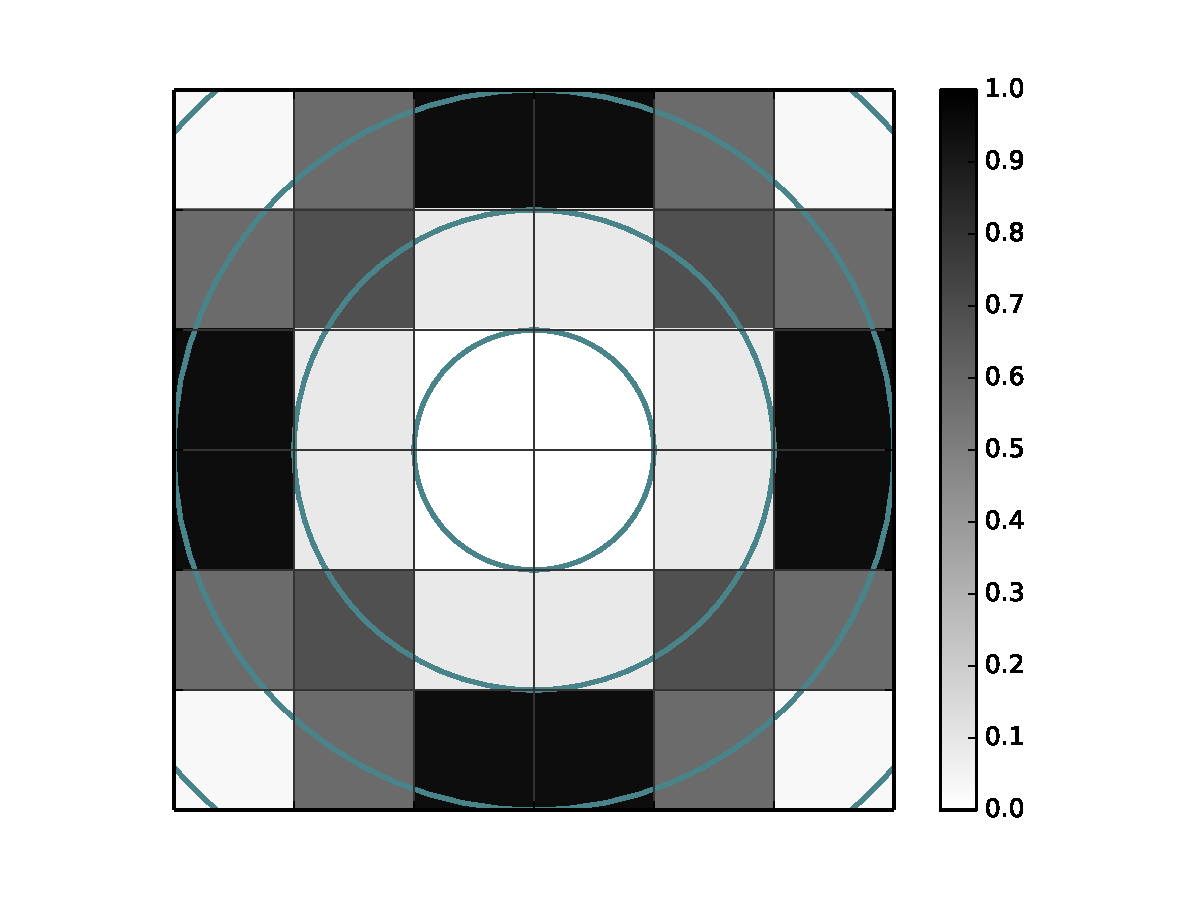
\includegraphics[height=0.39\linewidth]{figures/forceDistribution/radialDistribution/weights.pdf}
	\caption{Radial binning based on weighted contributions of intersecting cells. The fraction of cell's area that are within the third radial bin is color coded; black being 1 and white being 0.}
	\label{fig:radialBinningWeights}
\end{figure}


\noindent
On the same data set as used in figure \ref{fig:forceDistributions}, the computed radial distribution is as shown in figure \ref{fig:radialdistribution110000}.
The figure show the spatial distribution in polar coordinates (top row) and the radial average (bottom row) of the magnitude of force, normal force and shear force.
The normal force was found by treating the data as described in section \ref{sec:leastSquareRegression}.
What is meant by shear force is in this situation dependent on how we define it. 
Usually, the shear force is the component of contact force that is parallel to the contact surface (perpendicular to the normal force). 
However, by strictly using that definition, the computed shear force would have only positive contributions, and no notion of direction.
This would also not fit with the distributions derived by Hertz. 
Instead, we define the shear force as the radial component of the shear force as defined above.
Thus, if its general direction is away from the center of indentation, its value will  be positive, while if its towards the center it is negative. 
This way the shear force has a defined direction, but we no longer have the usual relation $\vec{F}=\vec{F_N} + \vec{F_s}$.
%These results will be discussed further in chapter \ref{sec:resultsRadialDistribution}.


\vspace{5mm}
\begin{figure}[H]
	\centering
	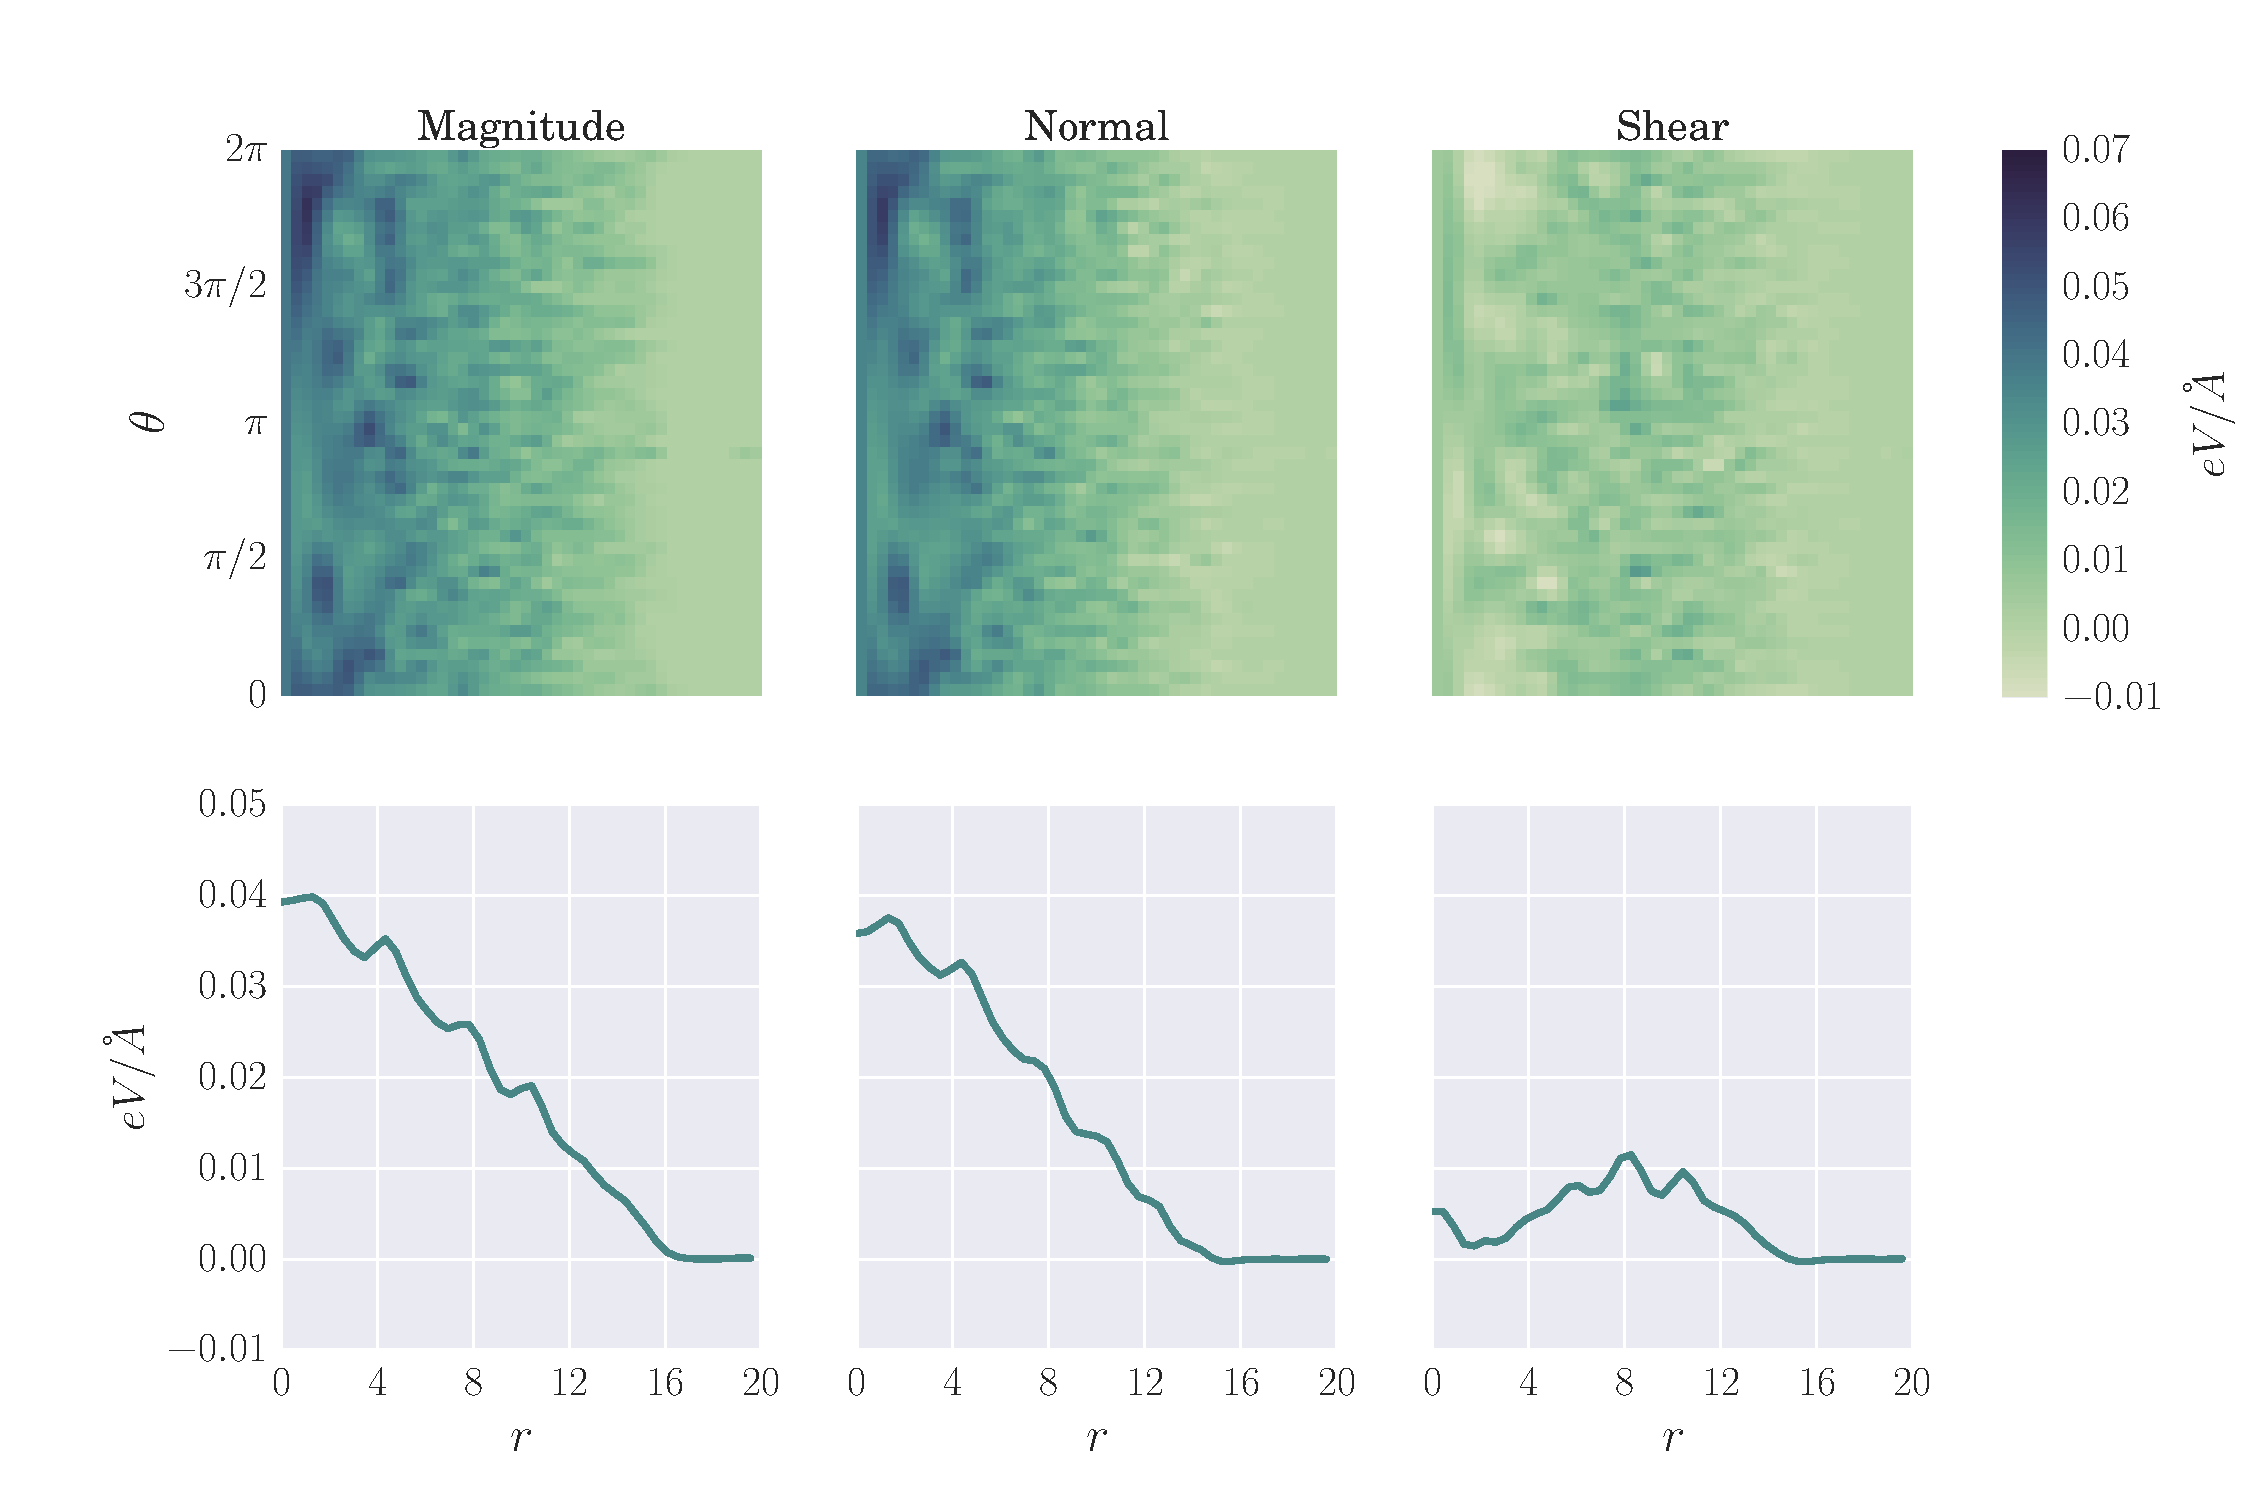
\includegraphics[width=\linewidth, trim={12mm 8mm 1mm 15mm}, clip]{figures/forceDistribution/forces/normalForceDistribution110000}
	\vspace{0mm}
	\caption{Spatial and radial distribution of the magnitude of force, as well as normal and shear force. 
		The spatial distributions shown on the top row are equivalent to the ones in figure \ref{fig:forceDistributions}, only in polar coordinates. 
		The value of the radial bins at a given radius $r$ in the figures at the bottom row, are the average value of the column at that $r$ in the top row.
		This figure show the result from a simulation where we push a sphere with radius of curvature $R=200\mathring{A}$,  40$\mathring{A}$ into a half-space of size $327.52\mathring{A} \times 327.52\mathring{A} \times 157.64 \mathring{A}$. This does not imply that the indentation is $40\mathring{A}$, but since contact was established, the top of the sphere has moved $40\mathring{A}$ towards the substrate. The real depth of indentation is less, due to deformations.}
	\label{fig:radialdistribution110000}
\end{figure}



\section{Results - Radial force distribution} \label{sec:resultsRadialForceDistribution}

\subsection{Specific description of experiment} \label{sec:resultsRadialForceDistributionSpecificDescriptionOfExperiment}
Using the methods described in this chapter we were able to monitor the contact force distribution, between the sphere and the substrate, during indentation. 
The sphere was initially positioned 20$\mathring{A}$ above the substrate, leaving no interaction forces between the two bodies.  
After equilibration the sphere was lowered at a constant rate of 0.5$\mathring{A}$/ps, by using the technique of deforming the simulation box. 
At the most, the sphere was lowered 60$\mathring{A}$, giving a depth of indentation of $h=40\mathring{A}$. 
The depth of indentation is here defined as if the sphere was perfectly rigid, unable to be deformed. 
Thus, a depth of indentation $h=20 \mathring{A}$ is the depth the sphere would indent had it been perfectly rigid. 
This is not the true depth, however. 
Due to elasticity the sphere deforms, leaving the indentation to be less than the listed value. 
A negative depth of indentation describe a separation between the sphere and substrate.   


Instead of using momentary measured values for the force distributions, we present the average distribution over a time-frame of 5000 time steps (10 ps). 
Thus, from we begin sampling until we stop, the (top of the) sphere has moved 5$\mathring{A}$ further down towards the substrate.  
During the 5000 time steps, we sampled every 5th step. 
Thus, a total of 1000 samples were used for every resulting mean distribution\footnote{This was achieved using  Nevery=5,  Nrepeat=1000 and Nfreq=5000 in line 3 of listing \ref{lst:usingCustomCompute}.}.

\subsection{Description of results}
The results from this simulation are shown in figure \ref{fig:resultsRadialForceDistributions}. 
The figure display the radial distribution of magnitude of contact force and the normal- and shear components, for a sequence of increasing depth of indentation $h$. 
The stated values of $h$ are the final values of the time-averages\footnote{For example $h=10\mathring{A}$ means the interval from $h=5\mathring{A}$ to $h=10\mathring{A}$.}.    
The first two intervals are not shown, since no interacting forces can be observed until $h=0\mathring{A}$, and so they look identical to the interval at $h=-5\mathring{A}$.
The x-axis represents radial distance $r$ from the center of indentation, in units of the unit cell length of $\beta$-cristobalite (7.12$\mathring{A}$). 
The sign of the force components indicate their direction.
A positive normal force indicates a repulsive normal component, and a negative normal force an attractive normal component. 
The shear force is defined as the component of the traditionally defined shear force that is in the radial direction. 
A positive sign indicates that the shear component is directed away from the center of indentation.
Likewise, a negative sign imply that the direction is towards the center. 
Numeric value of the forces are to be considered the average force acting on atoms of one of the bodies by atoms of the other body, at given radial distance. 


\begin{table}[H] 
	\begin{tabular}{cr} 
		h $[\mathring{A}]$ & \hspace{26mm}Magnitude \hspace{18mm} Normal \hspace{23mm} Shear \hspace{10mm} \\
		\toprule 
	
		-5 & \parbox[c]{0.83\linewidth}{
			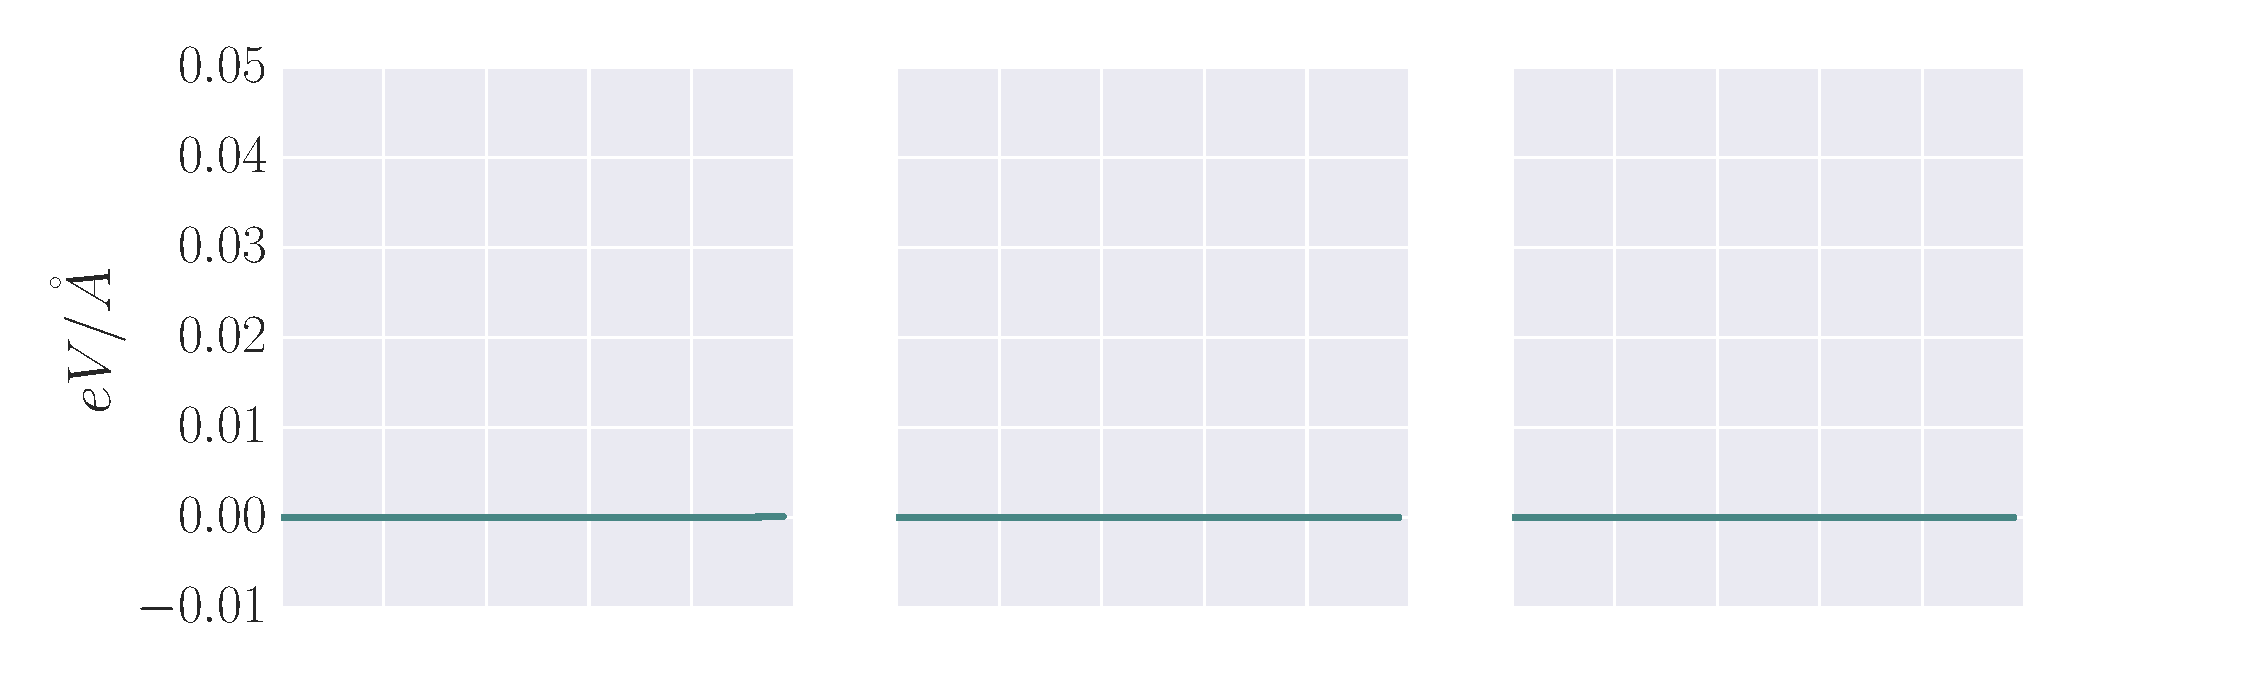
\includegraphics[width=\linewidth, trim={8mm 5mm 35mm 0}, clip]{../SiO2/xOneEighty/lower/5000/pythonScripts/timeSteps/radialOnly/timestep065000_bottom_without.pdf}
		}\\
	
		0 & \parbox[c]{0.83\linewidth}{
			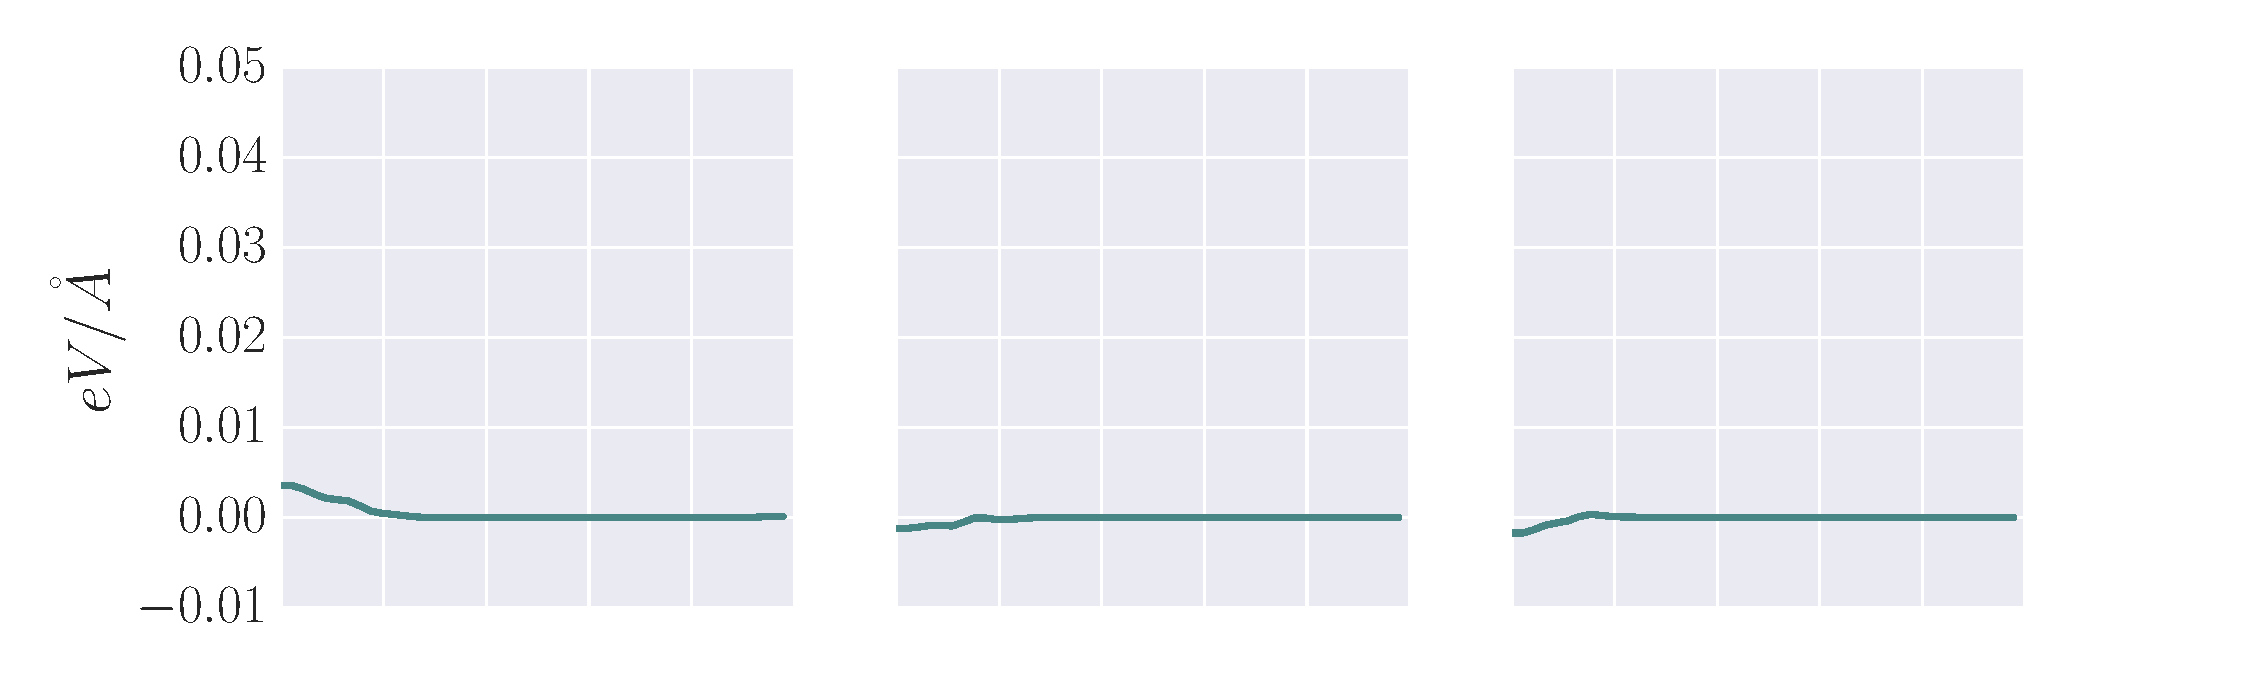
\includegraphics[width=\linewidth, trim={8mm 5mm 35mm 0}, clip]{../SiO2/xOneEighty/lower/5000/pythonScripts/timeSteps/radialOnly/timestep070000_bottom_without.pdf}
		}\\
	
		5 & \parbox[c]{0.83\linewidth}{
			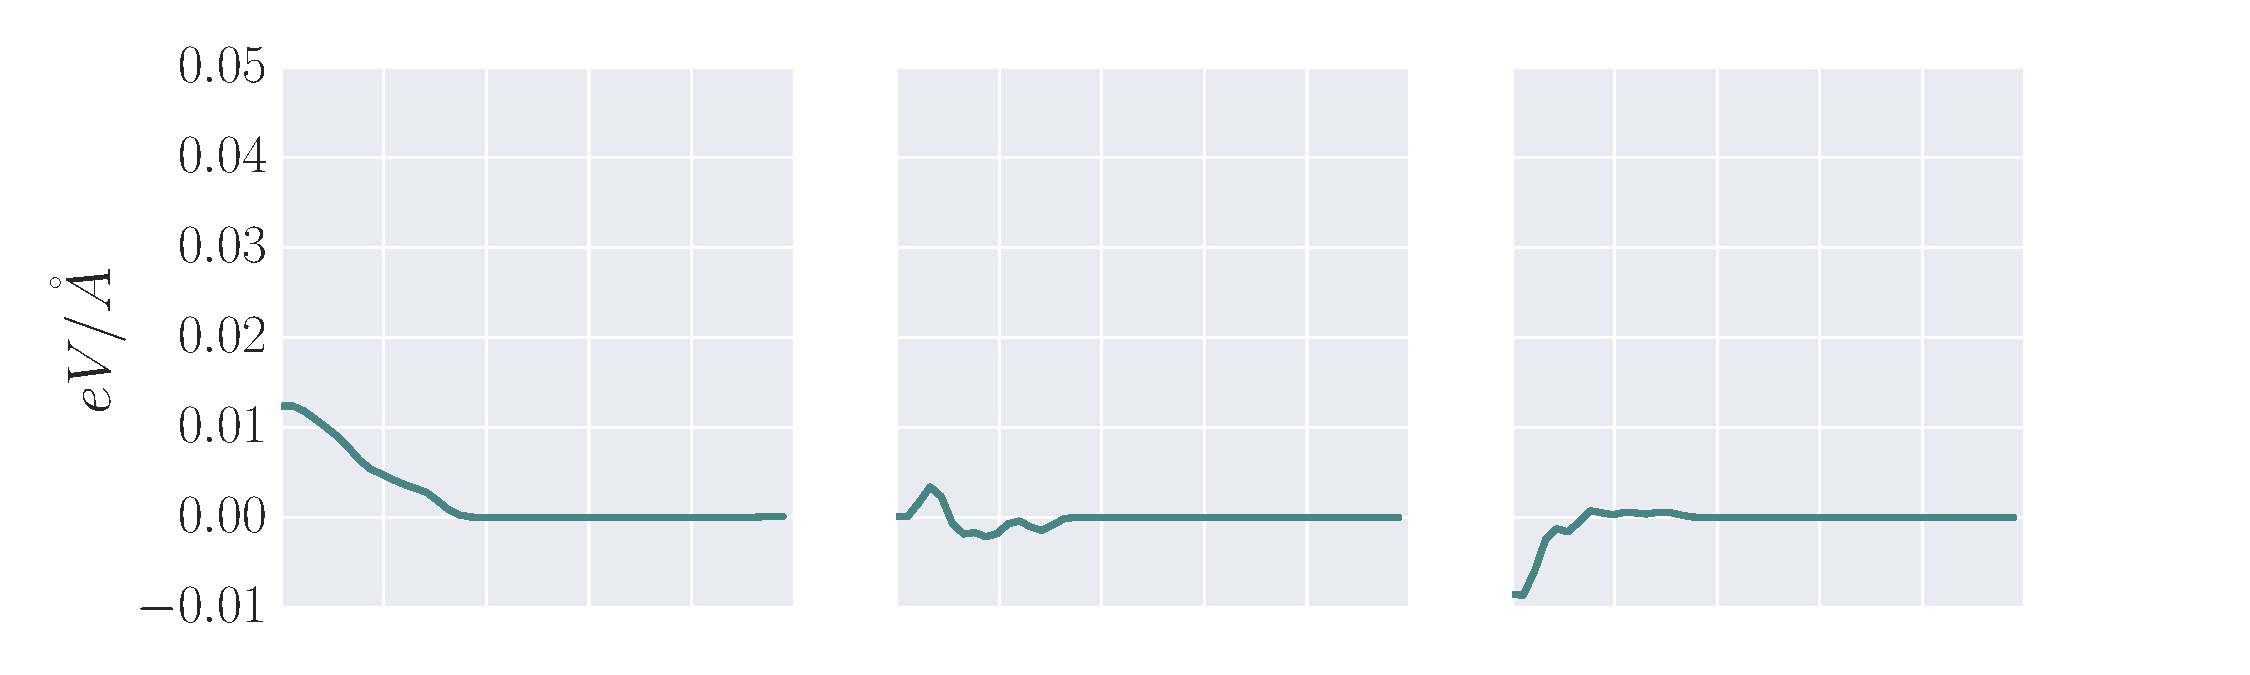
\includegraphics[width=\linewidth, trim={8mm 5mm 35mm 0}, clip]{../SiO2/xOneEighty/lower/5000/pythonScripts/timeSteps/radialOnly/timestep075000_bottom_without.pdf}
		}\\
	
		10 & \parbox[c]{0.83\linewidth}{
			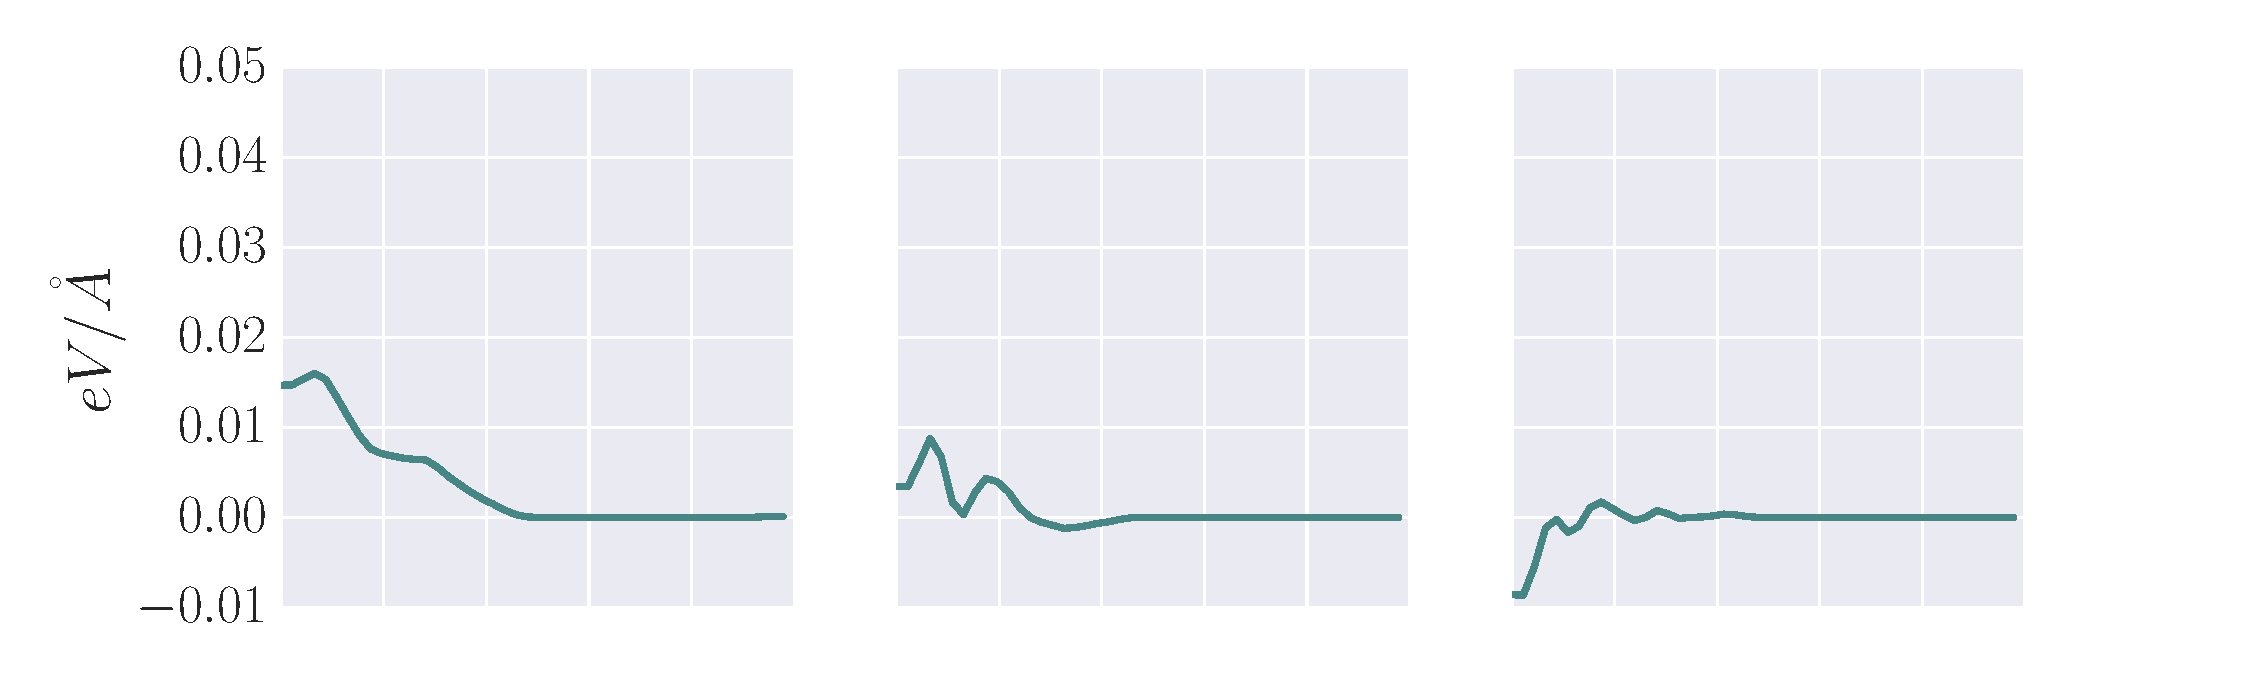
\includegraphics[width=\linewidth, trim={8mm 5mm 35mm 0}, clip]{../SiO2/xOneEighty/lower/5000/pythonScripts/timeSteps/radialOnly/timestep080000_bottom_without.pdf}
		}\\	
	
		15 & \parbox[c]{0.83\linewidth}{
			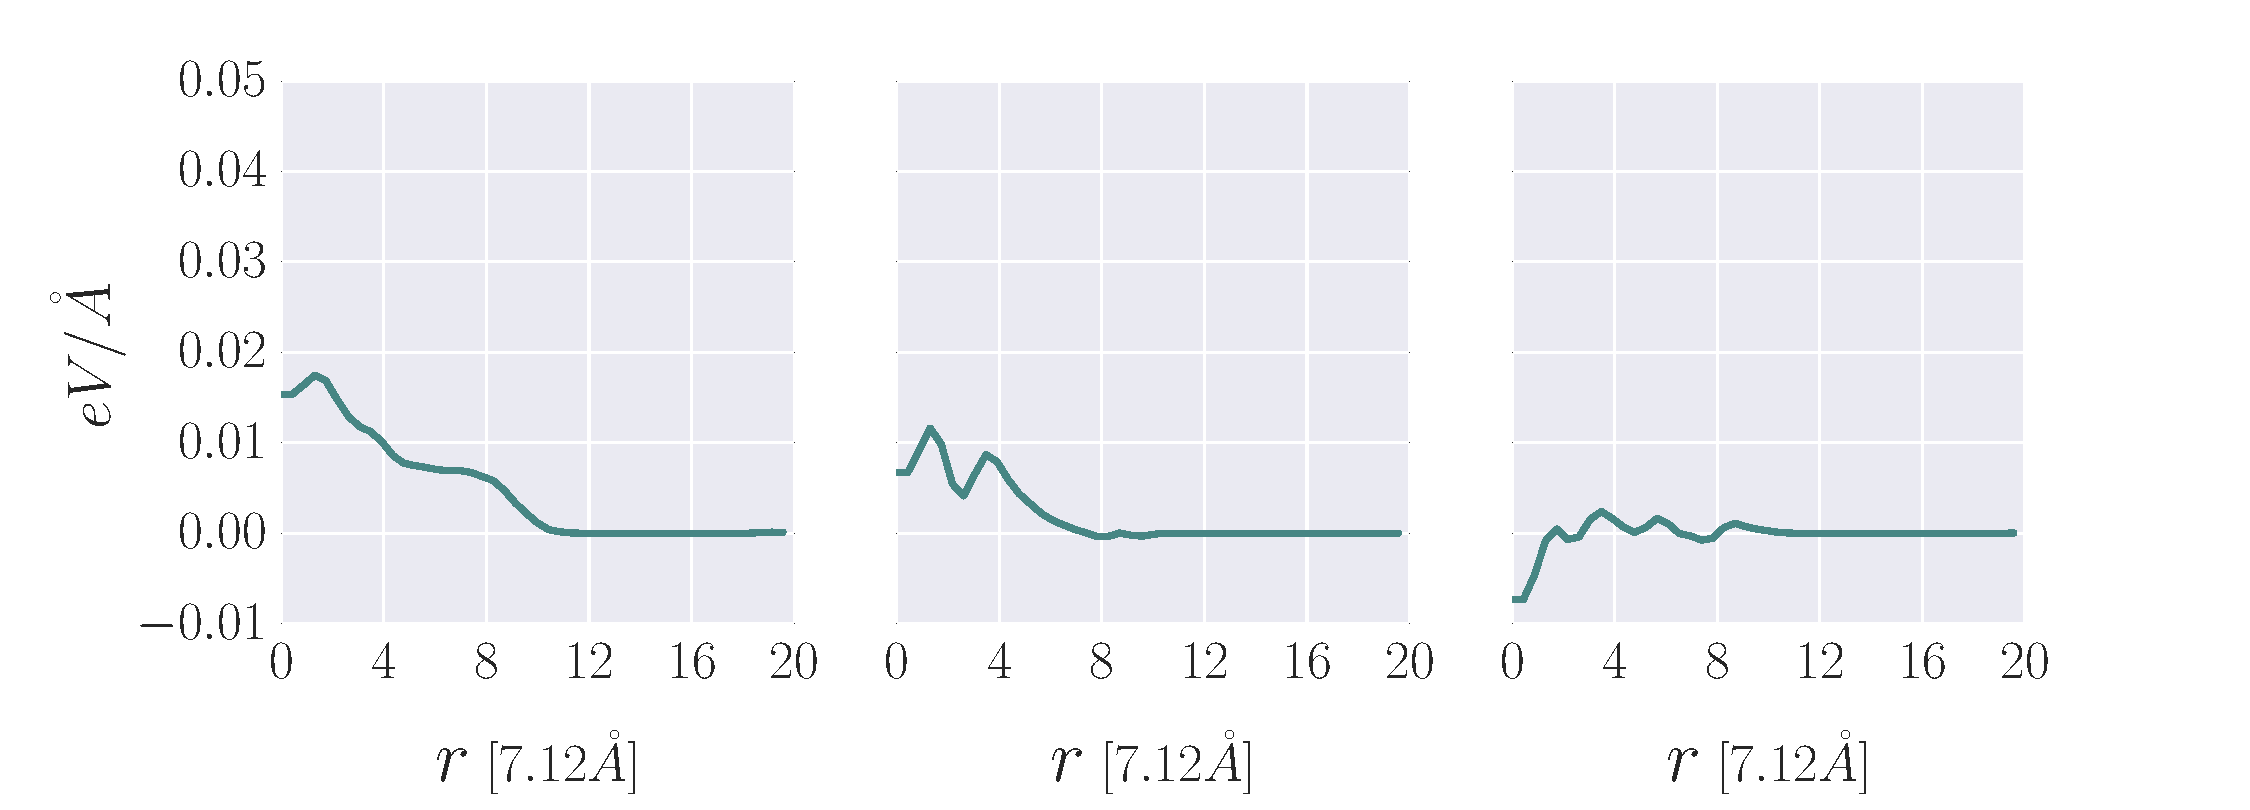
\includegraphics[width=\linewidth, trim={8mm 0 35mm 3mm}, clip]{../SiO2/xOneEighty/lower/5000/pythonScripts/timeSteps/radialOnly/timestep085000_bottom.pdf}
		}\\
	\end{tabular}
\end{table}

\begin{table}[H] 
	\begin{tabular}{cr} 
		h $[\mathring{A}]$ & \hspace{26mm}Magnitude \hspace{18mm} Normal \hspace{23mm} Shear \hspace{10mm} \\
		\toprule 
		20 & \parbox[c]{0.83\linewidth}{
			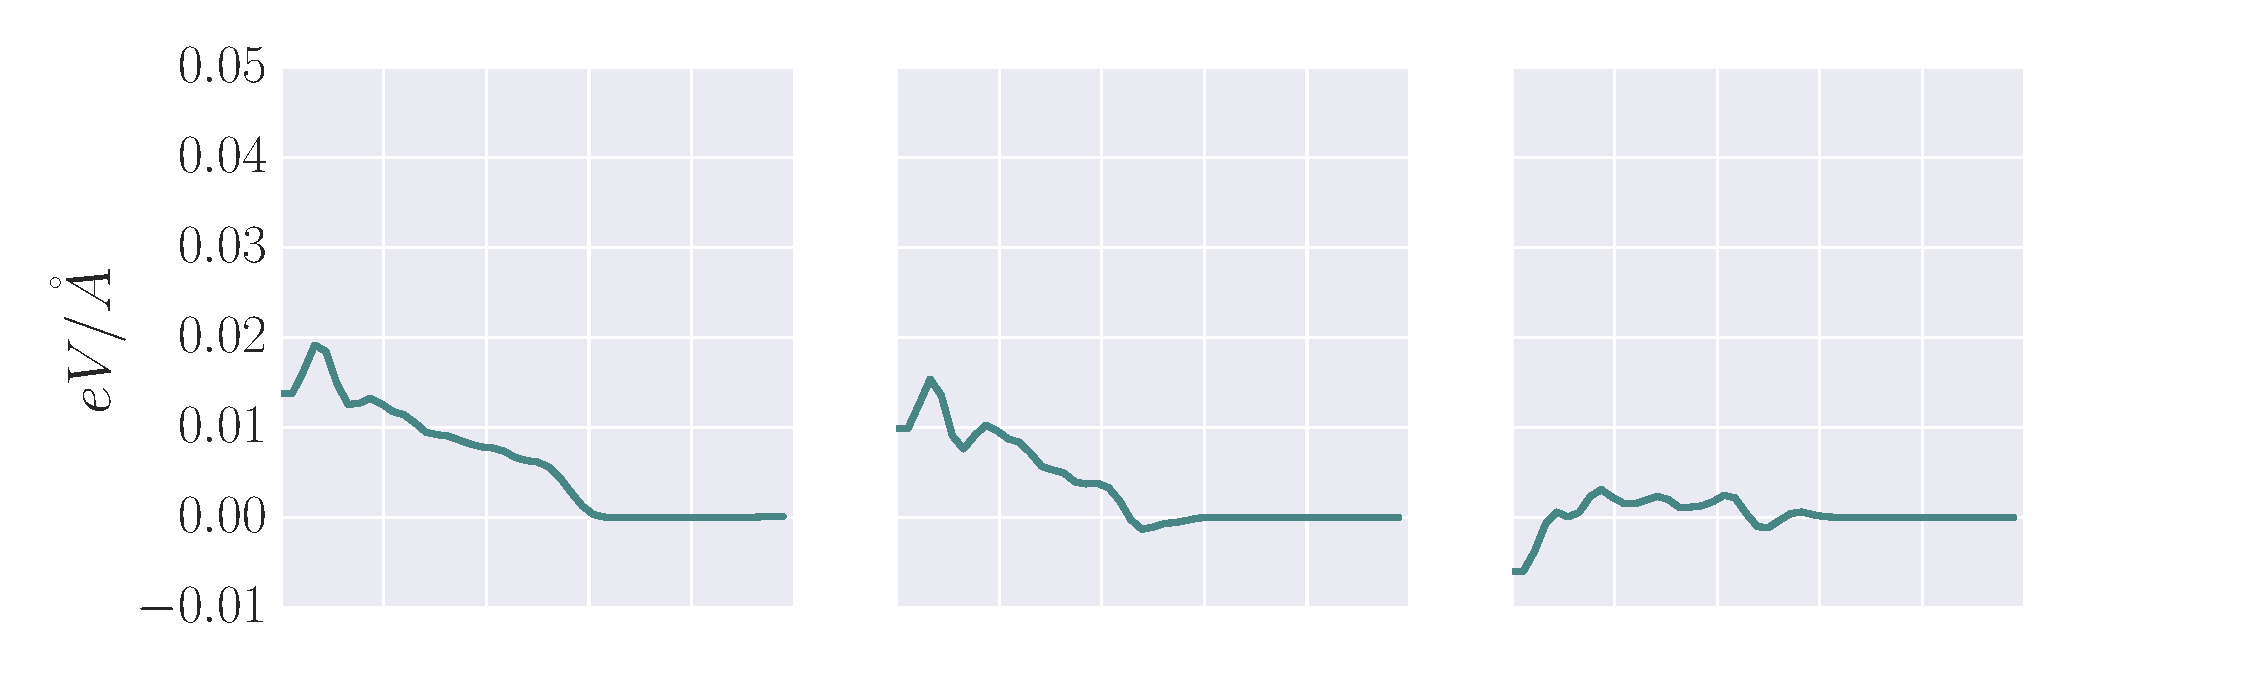
\includegraphics[width=\linewidth, trim={8mm 5mm 35mm 0}, clip]{../SiO2/xOneEighty/lower/5000/pythonScripts/timeSteps/radialOnly/timestep090000_bottom_without.pdf}
		}\\
		
		25 & \parbox[c]{0.83\linewidth}{
			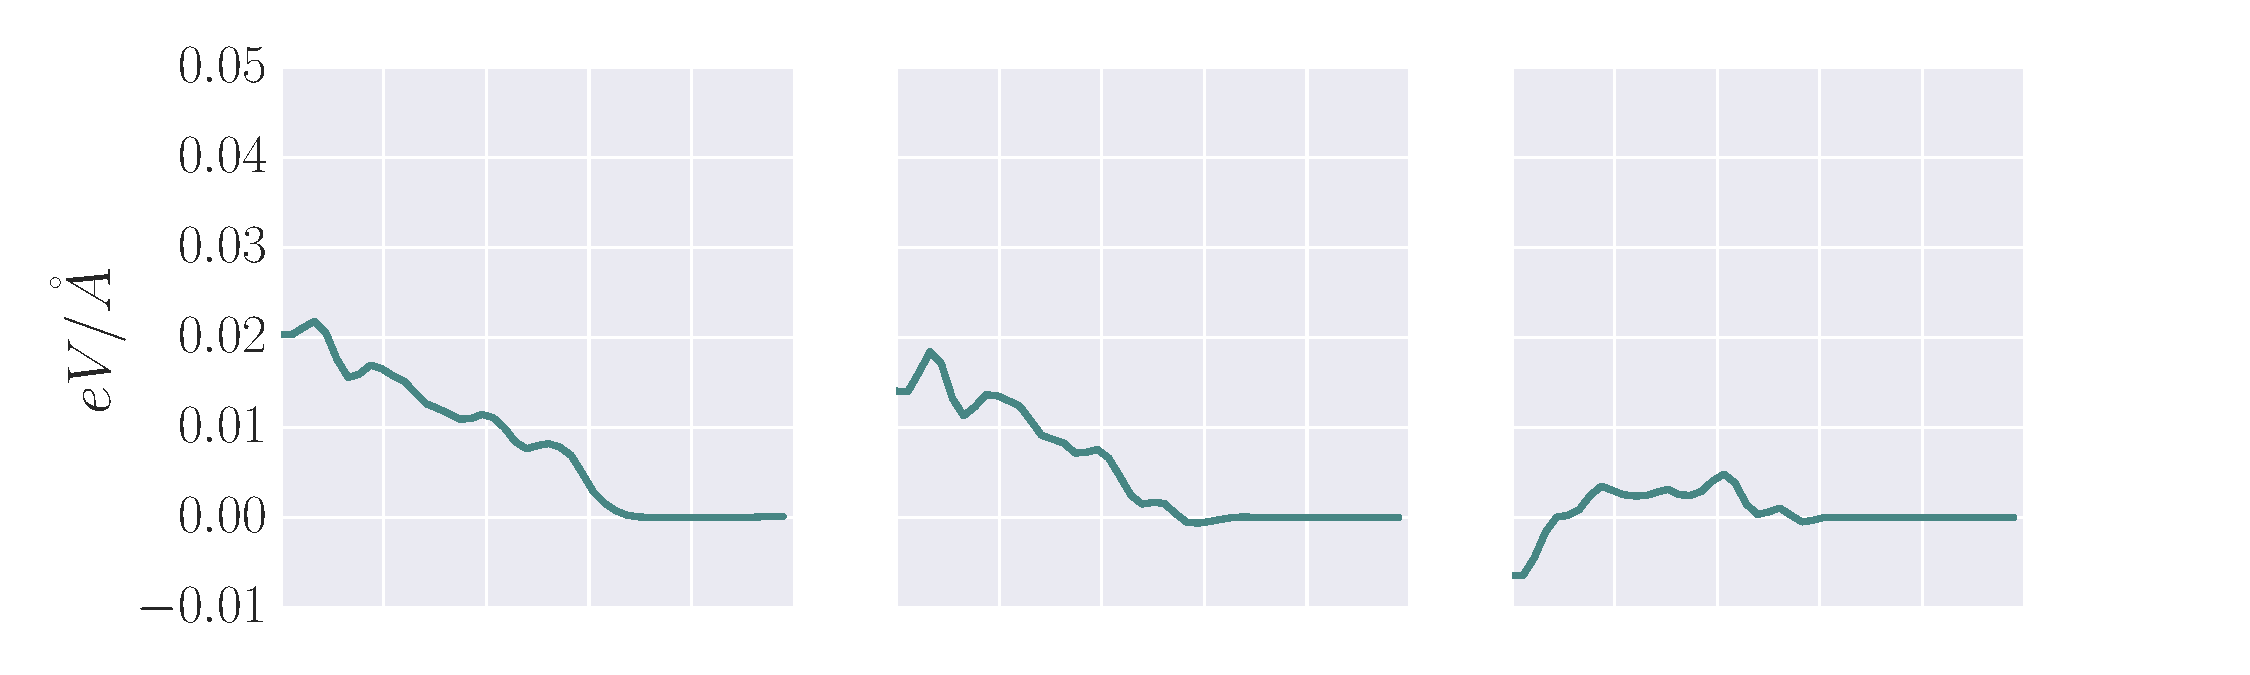
\includegraphics[width=\linewidth, trim={8mm 5mm 35mm 0}, clip]{../SiO2/xOneEighty/lower/5000/pythonScripts/timeSteps/radialOnly/timestep095000_bottom_without.pdf}
		}\\
		
		30 & \parbox[c]{0.83\linewidth}{
			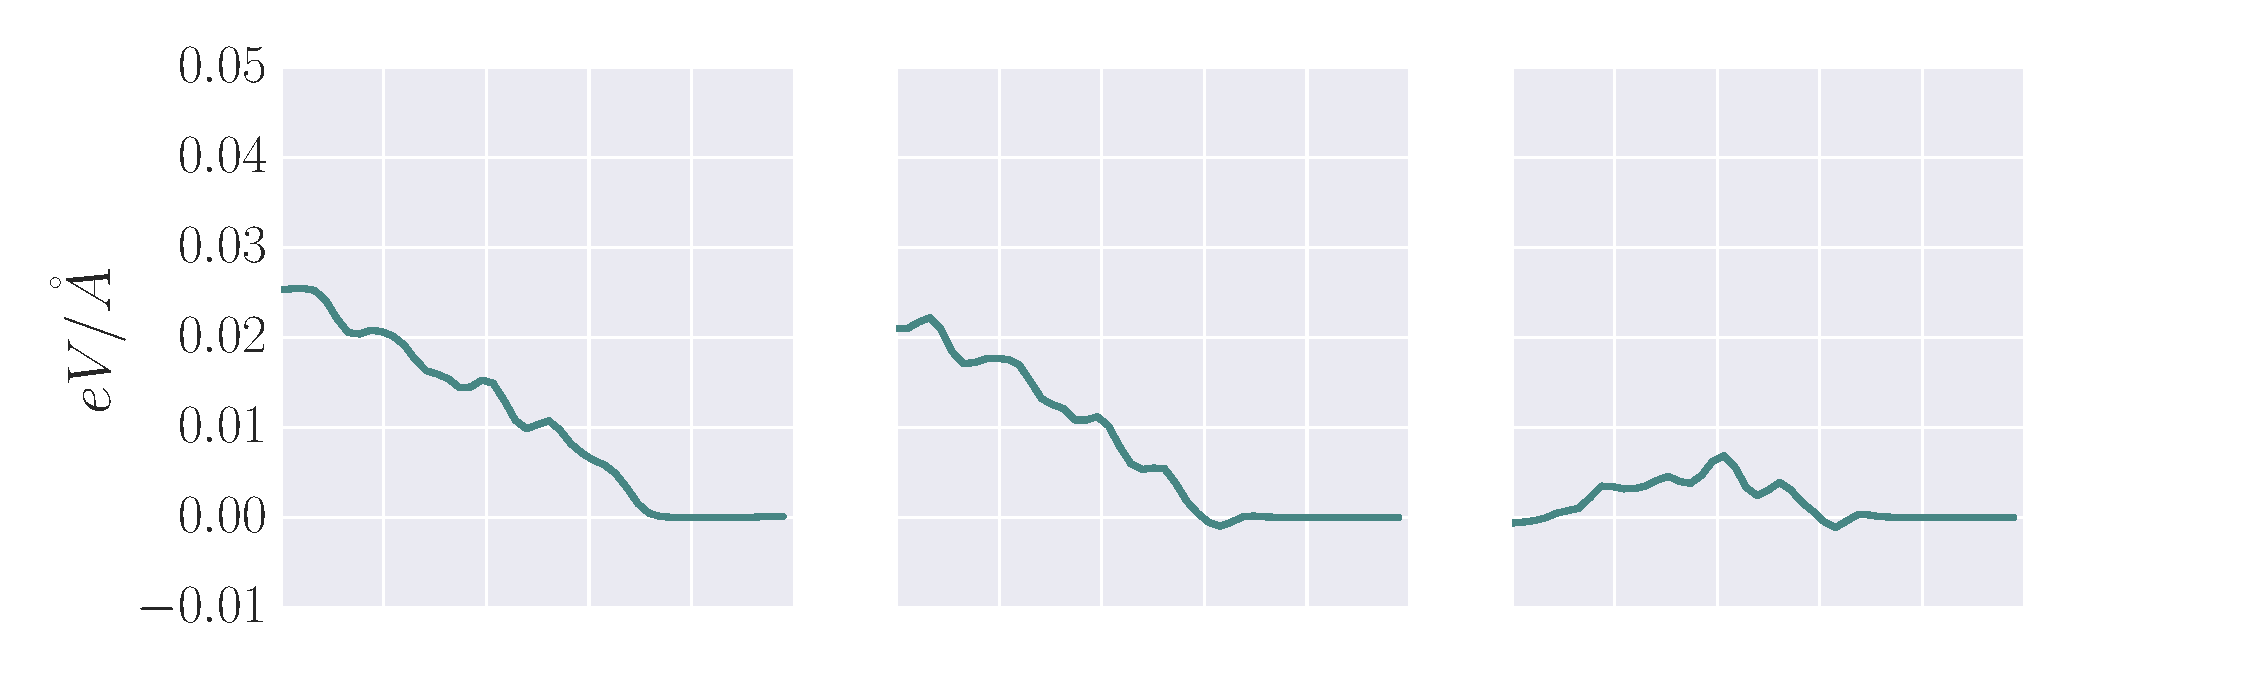
\includegraphics[width=\linewidth, trim={8mm 5mm 35mm 0}, clip]{../SiO2/xOneEighty/lower/5000/pythonScripts/timeSteps/radialOnly/timestep100000_bottom_without.pdf}
		}\\
		
		35 & \parbox[c]{0.83\linewidth}{
			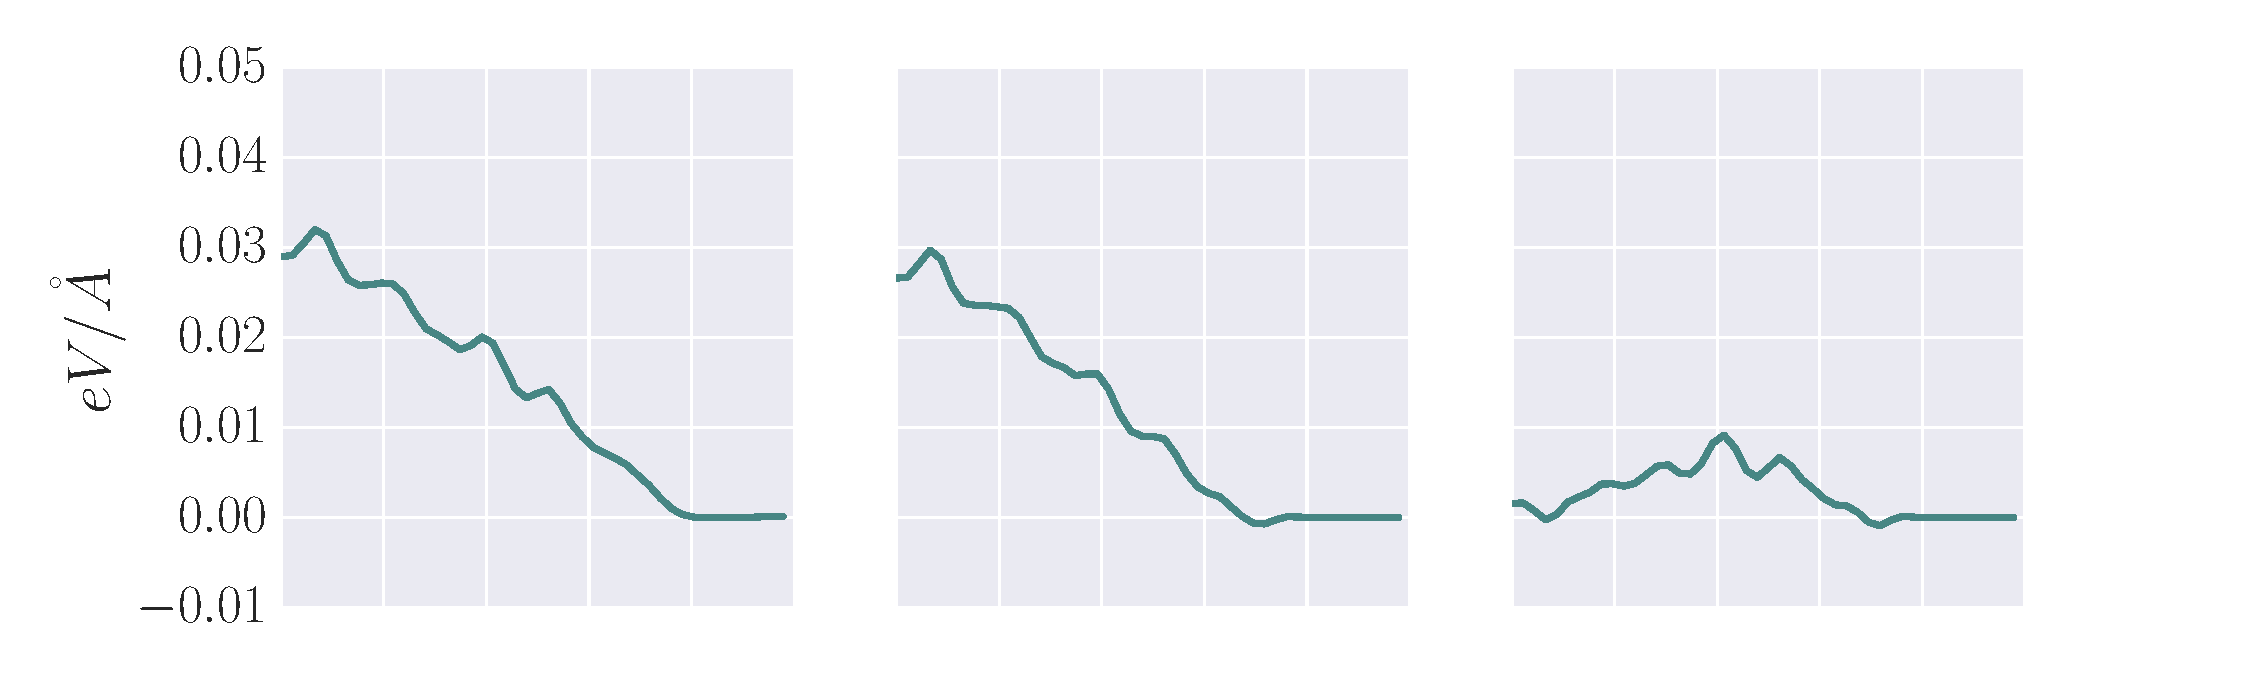
\includegraphics[width=\linewidth, trim={8mm 5mm 35mm 0}, clip]{../SiO2/xOneEighty/lower/5000/pythonScripts/timeSteps/radialOnly/timestep105000_bottom_without.pdf}
		}\\
		
		40 & \parbox[c]{0.83\linewidth}{
			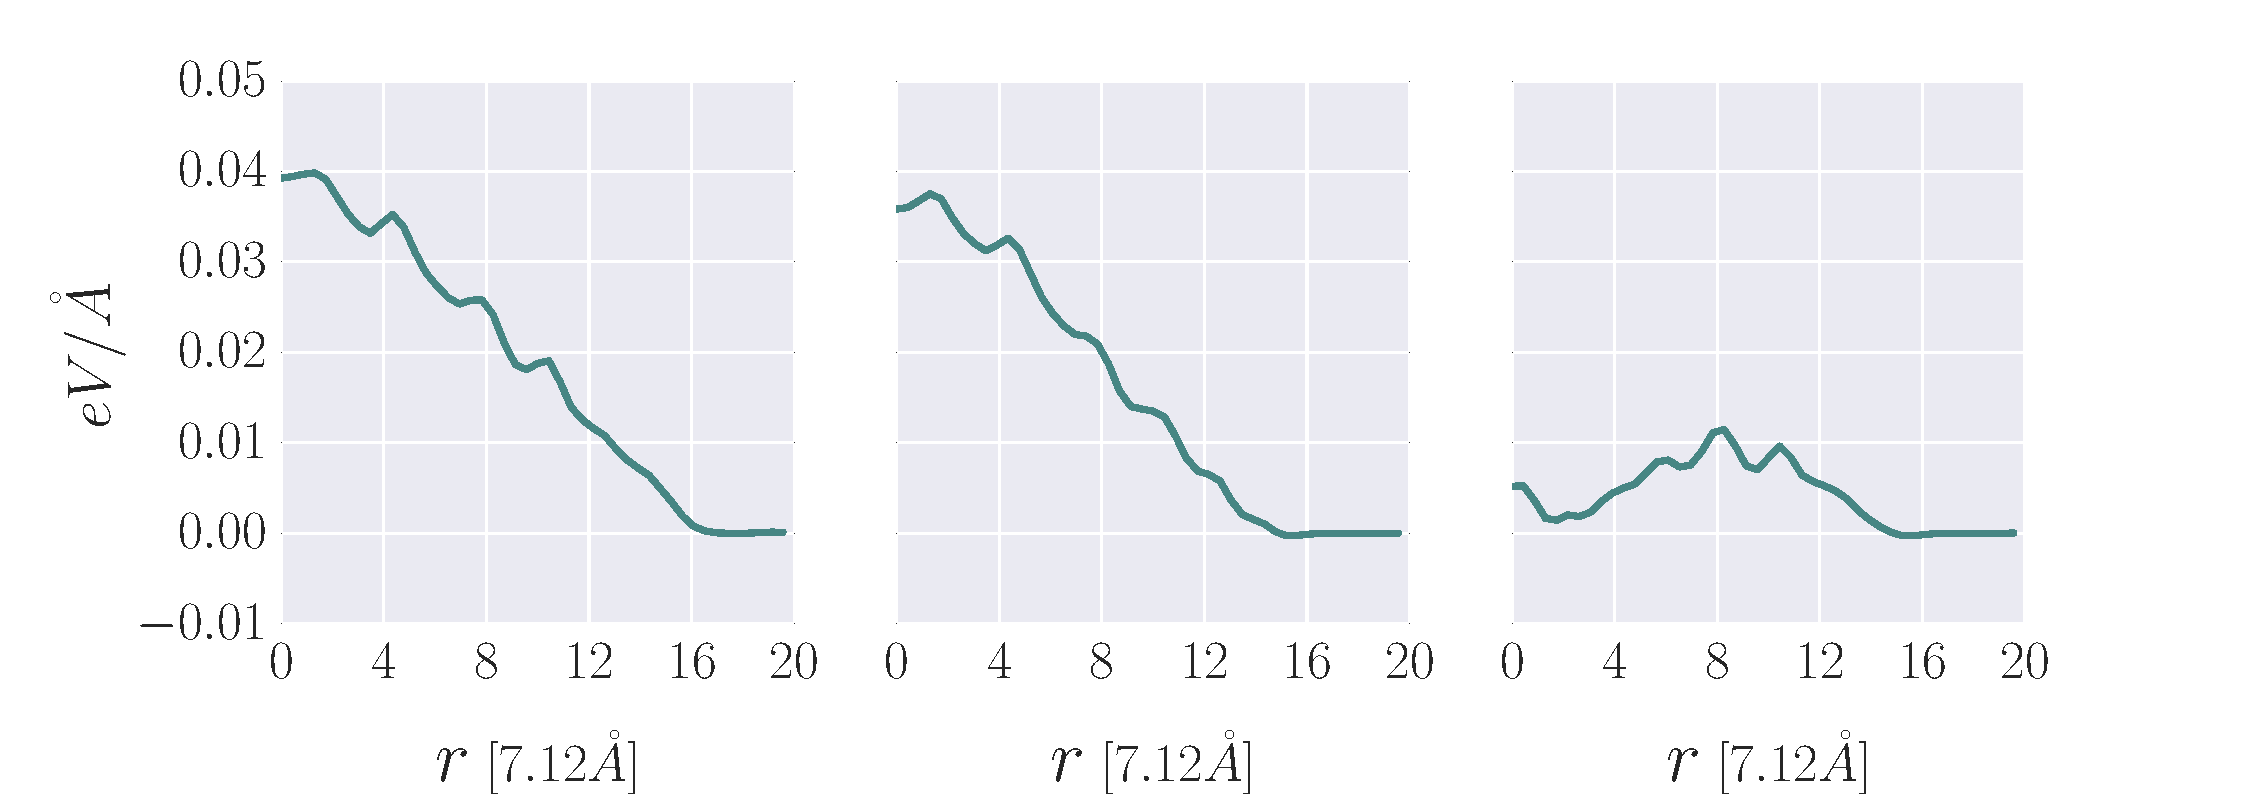
\includegraphics[width=\linewidth, trim={8mm 0 35mm 3mm}, clip]{../SiO2/xOneEighty/lower/5000/pythonScripts/timeSteps/radialOnly/timestep110000_bottom.pdf}
		}\\
		
	\end{tabular}
\end{table}
\begin{figure}[H]
	\caption{Radial distribution of contact forces acting on a sphere with radius of curvature $R=200\mathring{A}$ by a substrate of size $327.52\mathring{A} \times 327.52\mathring{A} \times 156.64\mathring{A}$ at different depths of indentation $h$. 
		Both bodies are made of $\beta$-cristobalite.
		The radial values are given in units of the unit cell length of $\beta$-cristobalite i.e. $7.12\mathring{A}$. 
		The depth of indentation is defined as if the sphere was perfectly rigid. 
		$h=0\mathring{A}$ being the initial point of contact, $h>0\mathring{A}$ being an indentation, and $h<0\mathring{A}$ distance between the surface of the substrate and the lowest point of the sphere. 
		Since the sphere isn't perfectly rigid it deforms and the depths of indentation aren't really as large as the values suggest. 	 		
		A positive normal force imply a repulsive force between the bodies, while a negative normal force imply an attractive force. 
		A positive shear force imply the force to be directed away from the center of indentation, and a negative shear force imply it to be directed toward the center. 
		This way of defining the shear force scales its true value to the component in the radial direction.
		Hence, with the shear force $\vec{F}_S$ we have defined here, we have $\vec{F} \neq \vec{F}_N + \vec{F}_S$.
}
\label{fig:resultsRadialForceDistributions}
\end{figure}

\noindent
 We do not detect any interacting forces between the two bodies until we reach the interval $h=-5$ to $h=0$, shown in the second row of the figure. 
 At this interval we see a small negative value in the normal force, indicating a weak attractive force. 
 Also, the shear force is negative, meaning the shear force is directed towards the center. 
 As the sphere is pushed farther towards/into the substrate the contact forces rise in magnitude, and both the normal- and shear force gain positive contributions. 
 
 We notice the normal force to have its maximum value close to the center for all intervals after repulsive forces are established. 
 Theoretically the maximum normal force should be right at the center. 
 However, this is not what we observe. 
 There seems to be a systematic dip in the normal force right at the center. 
 Had the dip not been systematic we could probably blame the discrepancy on bad statistics, considering the number of contribution to the average is very small near the center, and increases as $\propto r$. 
 Since it isn't we cannot use that argument. 
%Explenation - dip in normal force.
 The exact cause of the behavior is difficult to pinpoint. 
 It may be caused by a wrong definition of the center of indentation in the post-processing; basically that we have placed the center incorrectly. 
 It could be a 	consequence of atomic structure. 
 Both the sphere and the substrate are made of the same material, with the same crystalline structure. 
 The sphere was simply carved out, without any consideration to its structure or broken bonds. 
 It seems reasonable to expect the sphere to move slightly in order to fit best possibly with the structure of the substrate, hence shifting the center of indentation from the expected position. 
 From figure \ref{fig:zForceDistribution} and figure \ref{fig:radialdistribution110000} it is not clear if the forces are larger on one side of the center, than another. 
 The fact that the shear force near the center seems to be unreasonably low for most of the intervals may also point to an erroneous placing of the center during post-processing.
 However, this shifts sign at the later stages. 
 Again, at this radial position there's bad foundation in the statistics, so I won't read too much into this, as it is not completely systematic. 
 %A possible improvement would be to compute the center of mass of the sphere cap, and use it to determine the center of indentation. 
 
 There is another systematic dip in the radial normal distribution. 
 The rightmost non-zero value imply a small attractive force between the bodies. 
 This behavior was expected. 
 The parts of the  bodies that we macroscopically would consider not in contact are attracted by each other. 
 We can see from the figure how its radial position moves outwards as the indentation depth increases.
 From this we could estimate the area of contact to be within the  outermost radii where the normal force is positive.  
 This edge of the contact area is also possible to be seen in the radial distribution of shear force. 
 We see a negative value at the dip, because we study the force acting on the sphere from the substrate, leaving the attractive shear force outside the edge to be towards the center. 
  
 We see that the distributions are not smooth, as in continuum mechanics.  
 %WHY?
 
 From Hertz' theory we would expect the radial normal force distribution to be circular. 
 This is not possible to conclude from the obtained results. 
 If anything, it seems linear.

 The shear force conforms much better with Hertz' theory.
 At least at the last intervals it is clear that the maximum value is at a radial distance half of the radii of contact, and is zero both at the center and outside the edge. 
 The discrepancy due to the dip at the edge has already been addressed. 
 
 


\section{Results - Hysteresis}
As a continuation of the simulation giving the resulting distributions shown in figure \ref{fig:resultsRadialForceDistributions}, we may rise the sphere as well and study the difference in force interaction between the two cases. 
This is known as hysteresis.
As the sphere has been lowered $60\mathring{A}$ we held it still for 2ps, before rising it at the same speed as it was lowered. 
The reason for the equilibration is to counteract effects of pressure waves. 
We time-average the momentary normal force distribution in the same way as when it was lowered (described in section \ref{sec:resultsRadialForceDistributionSpecificDescriptionOfExperiment}).
We want to study the total normal force acting between the two bodies, but this term is somewhat vague. 
Does \textit{total normal force} refer to the sum of the forces' z-component at the contact area, or the sum of local normal force contributions in the contact area? 
Macroscopically we would choose the sum of z-components, however here we choose the sum of local normal force contributions.
As we move the sphere at a predefined rate, we compare the value of the total normal force between the descending and ascending cases at the same depth of indentation.  
The result is shown in figure \ref{fig:hysteresis}, where the measured normal force while descending and ascending the sphere is shown by the lighter and darker curve, respectively. 


\begin{figure}[H]
\centering
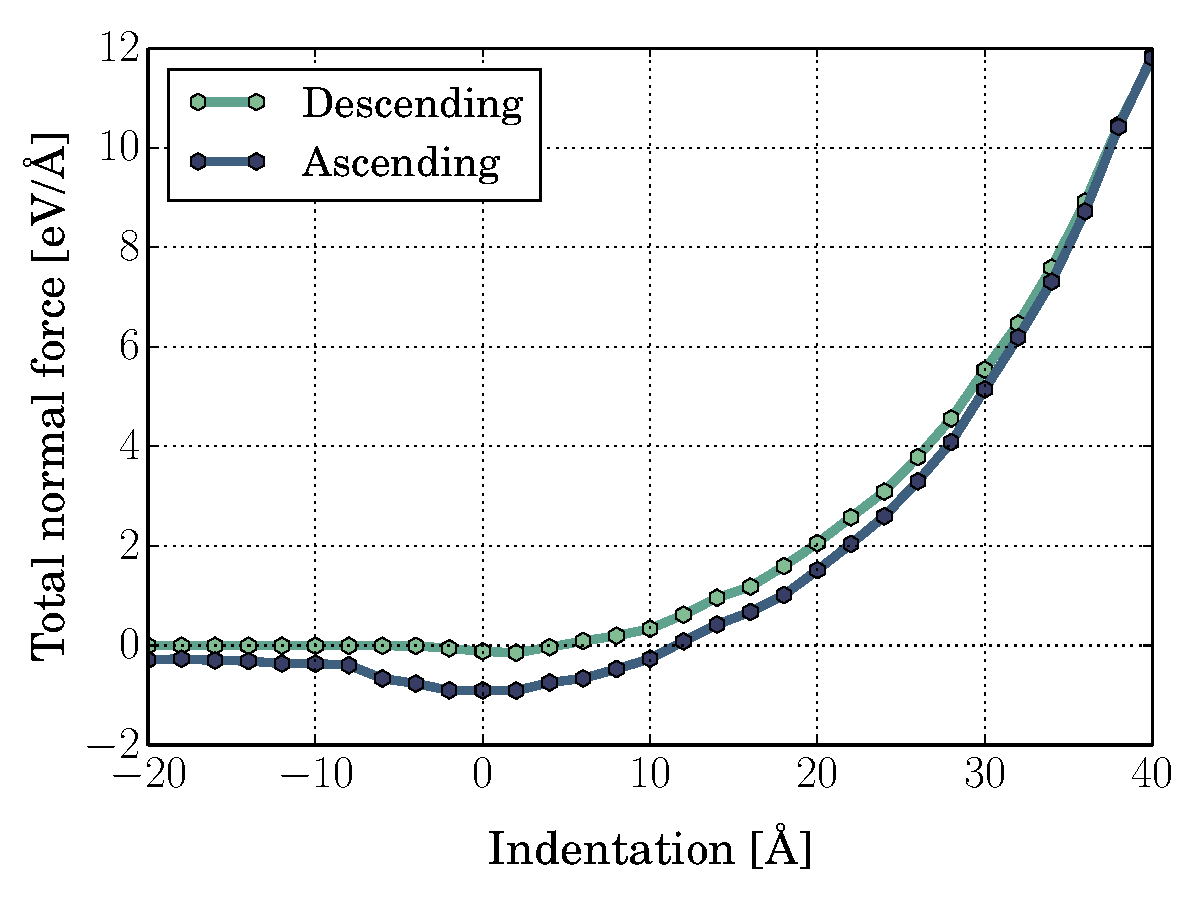
\includegraphics[width=0.7\linewidth]{figures/hysteresis/normal2}
\caption{
	Hysteresis plot obtained by simulating a sphere ... pushed down upon/into a flat substrate with constant velocity. 
	The total normal force is computed as the sum of all local normal components of contact force. The indentation is defined as zero where the tip of the sphere is at the same height as the surface of the substrate.
	The measured normal force while descending and ascending the sphere is shown by the lighter and darker curve, respectively. 
	After the sphere was lowered 60$\mathring{A}$, we equilibrated a short time before beginning the ascend.	
	Forces measured are averages of 1000 consecutive time points.
	Only every second measurement is shown, in order to not clatter the figure.  
	 }
\label{fig:hysteresis}
\end{figure}

\noindent
For identical height of the sphere, the measured normal force was greater during the descend than the ascend. 
This was an expected result and is due to friction. %adhesion.  
Atoms from the sphere and the substrate form bonds that counteracting the repulsive forces. 
Thus, resisting the sphere from rising. 
When ascending the sphere, these bonds must be broken.
%At the deepest indentation, the repulsive forces are much greater than those of adhesion, leaving them undetectable. 
The area between the two curves constitutes an energy loss, due to braking of these bonds.
The excess energy is dissipated as heat.

The two curves does not coincide at the height of initial contact (indentation height = 0). 
In fact, when ascending the two bodies seem to be in contact until the sphere has been elevated 10$\mathring{A}$ above the initial height of substrate surface. 
This is due to adhesion between the two bodies, as shown in the figure XX. 

For elevations above 10$\mathring{A}$, there is very little contact between the two bodies, and I suspect the measured normal force between them to not be due to these small contributions, but an effect of the method used. 
As the sphere ascends from the substrate, some atoms from the substrate may have attached to surface of the sphere. 
As we are rising the sphere at a constant velocity it makes sense that average force between atoms of the sphere and the attached substrate atoms are attractive. 
Though the atoms that initially was part of the substrate has become part of the sphere, the groups registered in LAMMPS were defined before that happened. 
As of now, the computes used do not accept dynamic groups, so this detail is not registered. 
However, as we can see this issue only result in a minor discrepancy. 





















\chapter{Computing the coefficient of static friction}
As described in section \ref{sec:coefficientOfFriction}, the coefficient of friction has a changing value depending on the relative motion of the bodies in contact. 
If they move (slide), the coefficient is usually significantly lower than if they are stationary. 
In our simulations, we have done the same experiment as described in said chapter, only in a molecular dynamics simulation. 
We will experience that the velocity\footnote{The velocity at which we pull the spring fixed to the spherical cap.} dependence of the static friction force $F_s$ impose a challenge in interpreting the results.
However, due to a clear linear dependence we are able to extrapolate $F_s$ for velocities approaching 0, which as we shall see, is a minimum limit for the static friction force. 

Once the method for finding the coefficient of static friction have been presented, we will study if/how it is dependent on the thickness of the substrate.

\section{Maintaining a normal force}
From the same simulation done when we pushed the sphere down onto the substrate, we systematically saved a restart file at every 10000 time step.
These can then be reloaded separately in order to compute the static force at different values of normal force.
Throughout the simulation, we must be certain to remain the normal force acting on the rigid top at the same value as when the restart file was written.
In our simulations we have used \texttt{fix addforce} with a constant value in the z-direction.
When lowering the sphere, the load was linearly increased. 
Because we change the circumstance from a linear increase to a sudden constant value, we equilibrate a short while before measuring, in order to avert effects of pressure waves.

\section{Adding a shear force}
In order to add a shear force, we fix a spring with stiffness $k$ to the rigid top layer of the sphere cap using the \texttt{Fix smd} command
 \begin{lstlisting}[language=LammpsInput, caption={LAMMPS command \texttt{Fix smd}, used to add a spring force to a group of atoms. The spring is considered fixed to the center of mass of the group and to a teatherd point, which we may move either with contant velocity of constant force.} ]
 fix ID sphereUpperG smd cvel ${k} ${v} tether 500 NULL NULL 0.0
 \end{lstlisting}
 which start out with the spring in its resting length, and begin pulling it with a constant velocity $v$ toward the position $x=500$. 
We disregard other dimensions, meaning we omit them from the distance computation and force application of the spring.
At this point there should be two external forces acting on the rigid top of the sphere cap: the normal force in the z-direction, and the spring force in the x-direction.
Each atom $i$ will be assigned an external force 
\begin{equation}
	\vec{F}_i = -k(\vec{r}_i- \vec{r}_0)\frac{m_i}{M},
\end{equation}
where $k$ is the spring constant, $\vec{r}_i$ and $\vec{r}_0$ are the position of atom $i$ and the tethered point, respectively, $m_i$ is the mass of atom $i$, and $M$ is the total mass of the group of atoms. 
As we only regard the x-dimension, the position vectors are evaluated as $\vec{r}_i=x_i$ and equivalently $\vec{r}_0 = x_0$.


\section{Procedure}
In the completed simulations we have used a time frame long enough for the spring force to start decreasing (slip). Typically they were of the order of 50000 time steps (0.1ns).
The procedure was equivalent for all time steps, only the velocity at which we pull the spring was increased between simulations. 
We increase the velocity between simulations because we expect the static force $F_s$ to increase when the normal force increases.
In order for the spring to exert a force equal to $F_s$, we have to extend the spring farther. 
By increasing the velocity at which we pull the spring we reduce the number of time steps needed, saving time and computational expense.
This can be seen in figure \ref{fig:springUnScaledExtension}.

\texttt{fix smd} computes 7 quantities, that are stored as a vector. 
As described in the documentation\footnote{\href{http://lammps.sandia.gov/doc/fix_smd.html}{\url{http://lammps.sandia.gov/doc/fix_smd.html}}}, 
these quantities are:  the x-, y-, and z-component of the pulling force, the total force in direction of the pull, the equilibrium distance of the spring, the distance between the two reference points, and finally the accumulated PMF (the sum of pulling forces times displacement), this order.
We are interested in the first value, i.e. the total pulling force component in the x-direction.
By setting up a custom format for the \textit{thermo\_style}, we consistently store the value of the total force component in the x-direction every 100 time step. 
This way, we can monitor the force applied by the spring as a function of time.

\section{Treating the results}
The result from a single simulation is shown in figure \ref{fig:springSingle_v3}.
\begin{figure}
	\centering
	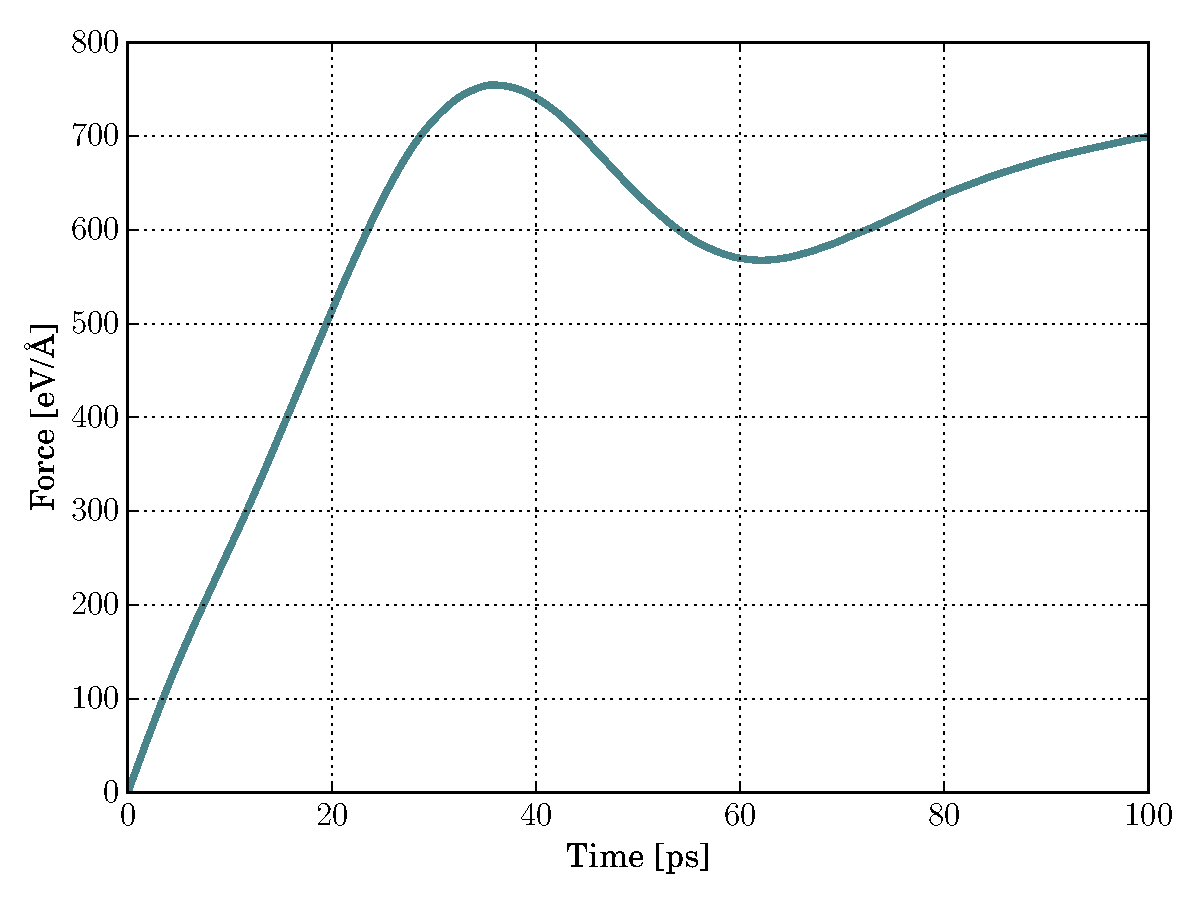
\includegraphics[width=0.7\linewidth]{figures/friction/scalingCoeffisient/single_v3}
	\caption{Spring force as a function of time, where we pull the spring by a constant velocity $v=3$~[\AA/ps].}
	\label{fig:springSingle_v3}
\end{figure}
\noindent
As we see, the spring force increases linearly as expected from Hooke's law. 
We are really only interested in finding the maximum value of spring force, namely the static friction $F_s$.
Since we know the value of the normal force, we may be enticed to compute the coefficient of static friction as $\mu=F_ s/N$ momentarily. 
However, this would be erroneous. 
It turns out that the static friction is dependent on the velocity at which we pull the spring. 
$F_s$ increases with the velocity.
Thus, the spring force will engage sliding at a lower value at slow pulling speeds, than at high.
This can be deduced from our results as well. 
Figure \ref{fig:springUnScaled} show the evolution of the spring force from 5 different simulations, all using a different velocity, and demonstrating that the maximum spring force is different in each case. 
We may rescale the x-axis by multiplying with the velocity to obtain the spring force as a function of the extension of the spring.  
So, how are we supposed to conclude a coefficient of friction from our simulations? 
The solution is to find the relation between the coefficient and the velocity.
By using the dataset shown in figure \ref{fig:springUnScaled} and \ref{fig:springUnScaledExtension} we may plot $\mu(v)$ by computing $\mu = F_s/N$ for every velocity.
The result is shown in figure \ref{fig:springUvsV}. 
The relation is obviously linear, at least for the considered range of velocities. 
By linear regression the approximated function for the velocity dependent coefficient of friction is 
\begin{equation}\label{eq:UofV}
	\mu(v) = 0.0702v + 0.3992.
\end{equation}
By rescaling the axis of figure \ref{fig:springUnScaledExtension} 
by this function, we get data collapse as shown in figure \ref{fig:springDataCollapse}. 
Note that we normalize the y-axis by dividing with the normal force $N$.
Collapse of the curves indicate that at all these velocities the system is subject to the same physical process. 
Had the curves been very distinguishable, we could conclude that there is some other effect taking place. 
These curves overlap quite nicely, so I do not see any cause of concern\footnote{Though this is a subjective opinion.}.
The collapse is not of use to us in the pursue of computing the coefficient of static friction. 
The result that is of real interest is the relation posed in equation \eqref{eq:UofV}. 
In macroscopic experiments the spring is loaded very slowly compared to the velocities we use when simulating. 
We really seek the value of $F_s/N$ when the velocity approaches zero.
This is the minimum ratio of shear force to normal force. 
In the case discussed it amounted to $F_s/N = 0.4$.

So now, for every value of the normal force, we need to take a series of simulations using different velocities.
It is not intuitive how $\mu(v)$ will change as we perturb $N$. 
However, we may still expect a linear dependence.
Figure \ref{fig:uvsn} show the result of one such series of simulations. 
For every point $(N,\mu(N))$ there was done 5 simulations using different velocities. 
The one shown in figure \ref{fig:springUvsV} is one at which the substrate had a depth XX and the normal force was XX.
The constant term in the linear approximations is the stored value of $\mu(N)$.
Obviously since $\mu = F_s/N$ we can multiply the y-axis of this figure to obtain the shear force versus normal force, as shown in figure \ref{fig:fvsn}.
Again we see a linear dependence, and may apply linear regression to obtain the relation.
\begin{equation}
	F_s(N) = 0.255N + 174.906
\end{equation}
which is very assuring, since this is in agreement with Amontons' law of friction. 
The slope of this line indicates the rate at which the shear force increases with increasing normal force. 
Thus, the slope of this line is the coefficient of static friction we have been looking for.
In this example case it was $\mu = 0.255$.



\raggedbottom
\newpage			% WATCH OUT!
\flushbottom



\begin{figure}[H]
\centering
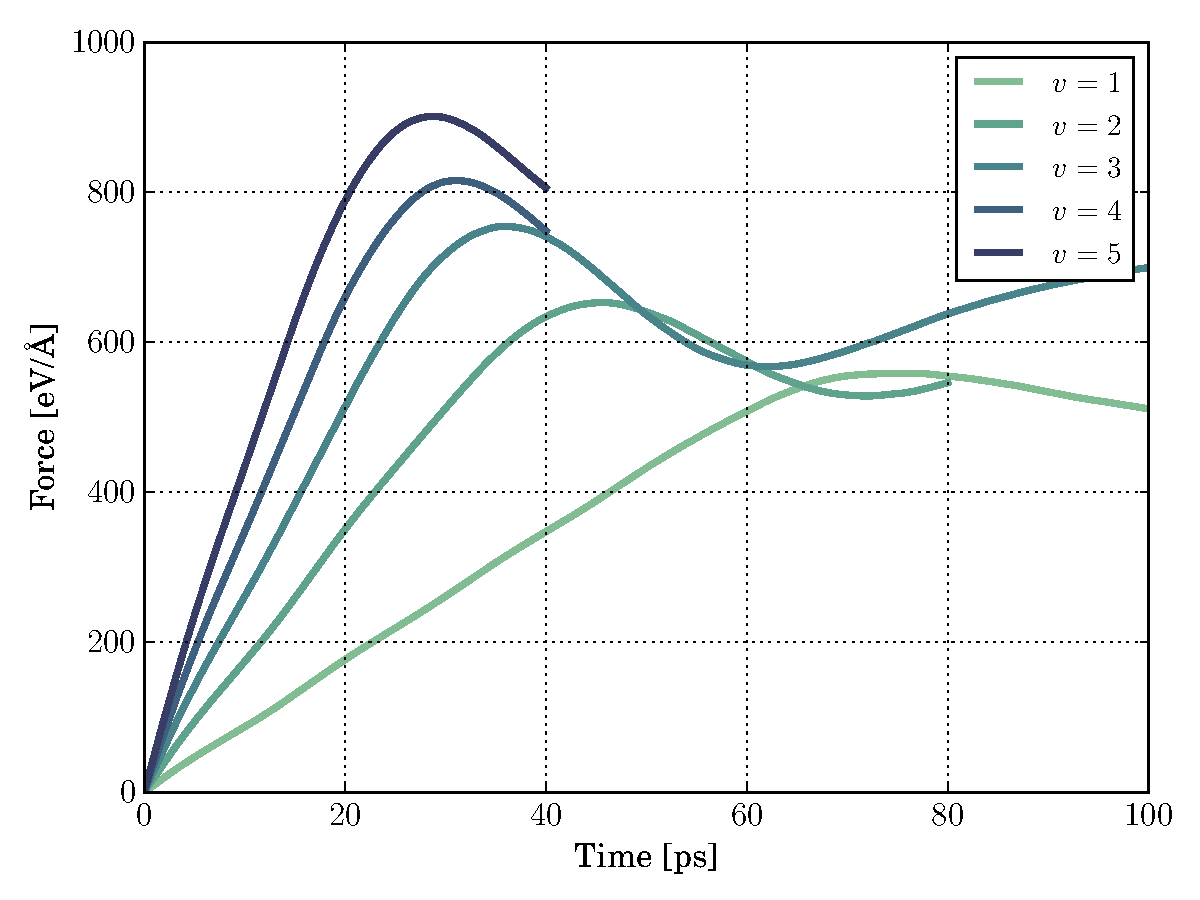
\includegraphics[width=0.7\linewidth]{figures/friction/scalingCoeffisient/UnScaledSliding}
\caption{Spring force as a function of time for several values of velocity.}
\label{fig:springUnScaled}
\end{figure}

\begin{figure}[H]
\centering
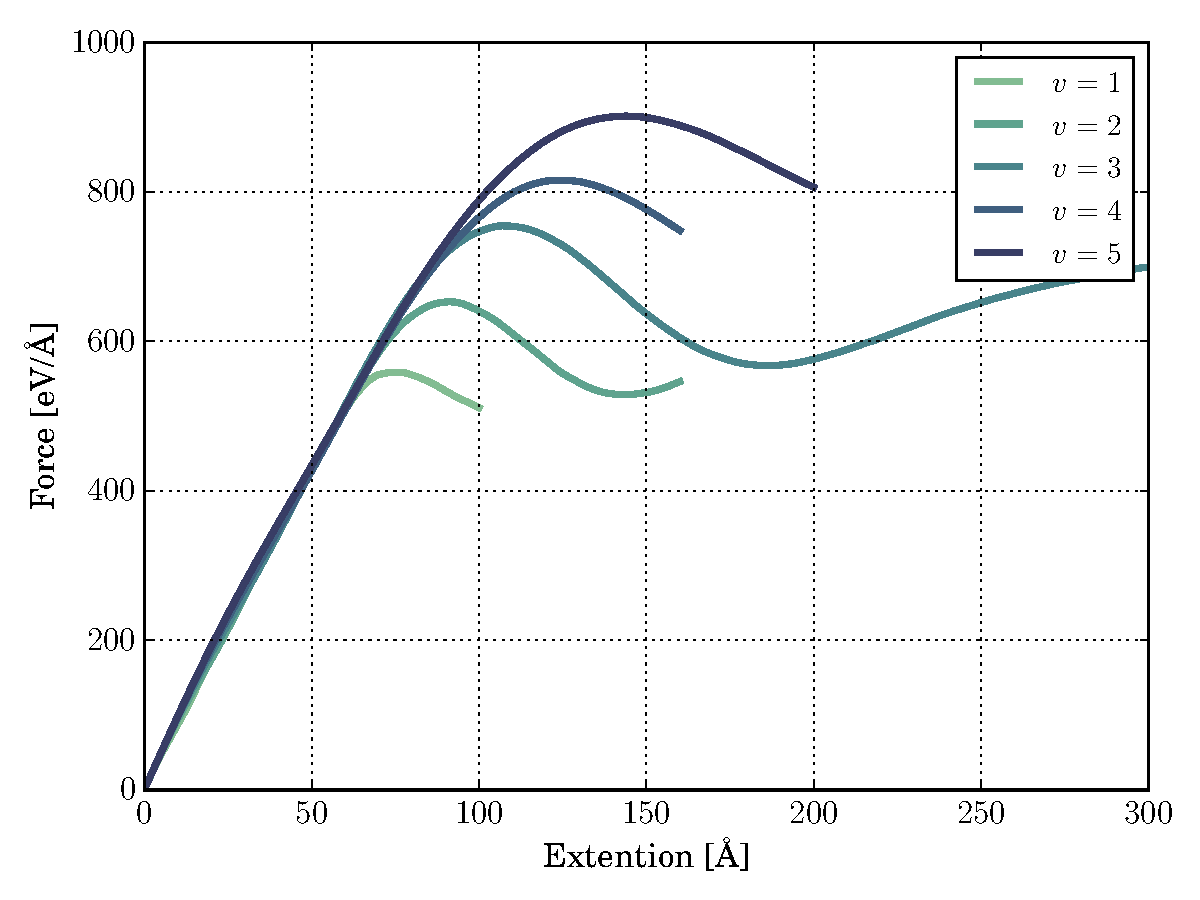
\includegraphics[width=0.7\linewidth]{figures/friction/scalingCoeffisient/UnScaledExtention}
\caption{Spring force as a function of the extension of the spring for several values of velocity.}
\label{fig:springUnScaledExtension}
\end{figure}

\begin{figure}[H]
\centering
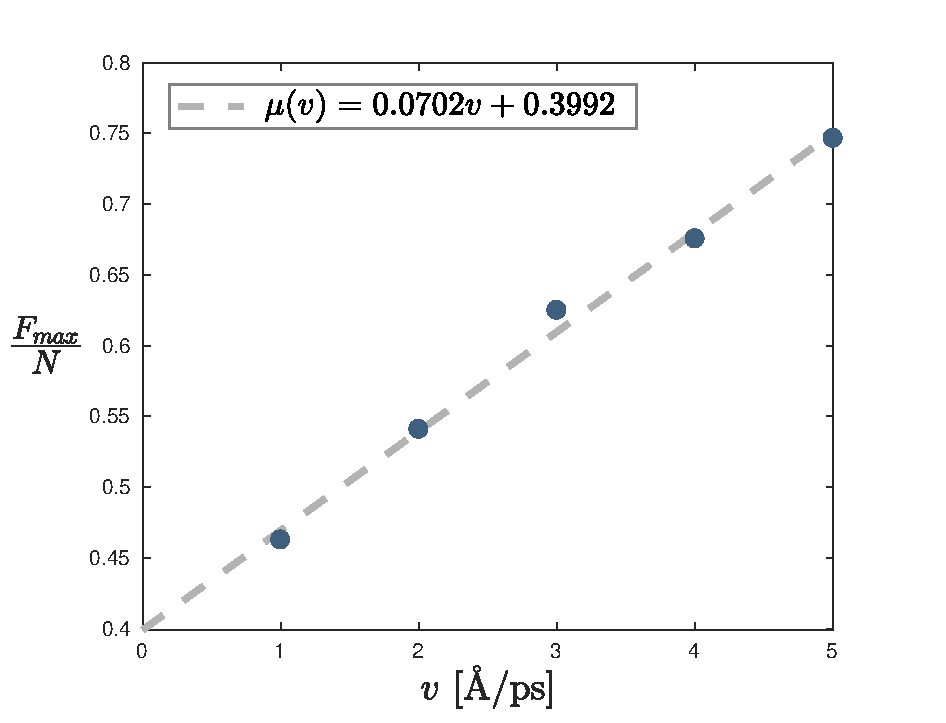
\includegraphics[width=0.7\linewidth]{figures/friction/scalingCoeffisient/u(v)}
\caption{Coefficient of friction $\mu$ as a function of velocity $v$. Linear regression is suited to approximate the relation $\mu(v)$.}
\label{fig:springUvsV}
\end{figure}

\begin{figure}[H]
\centering
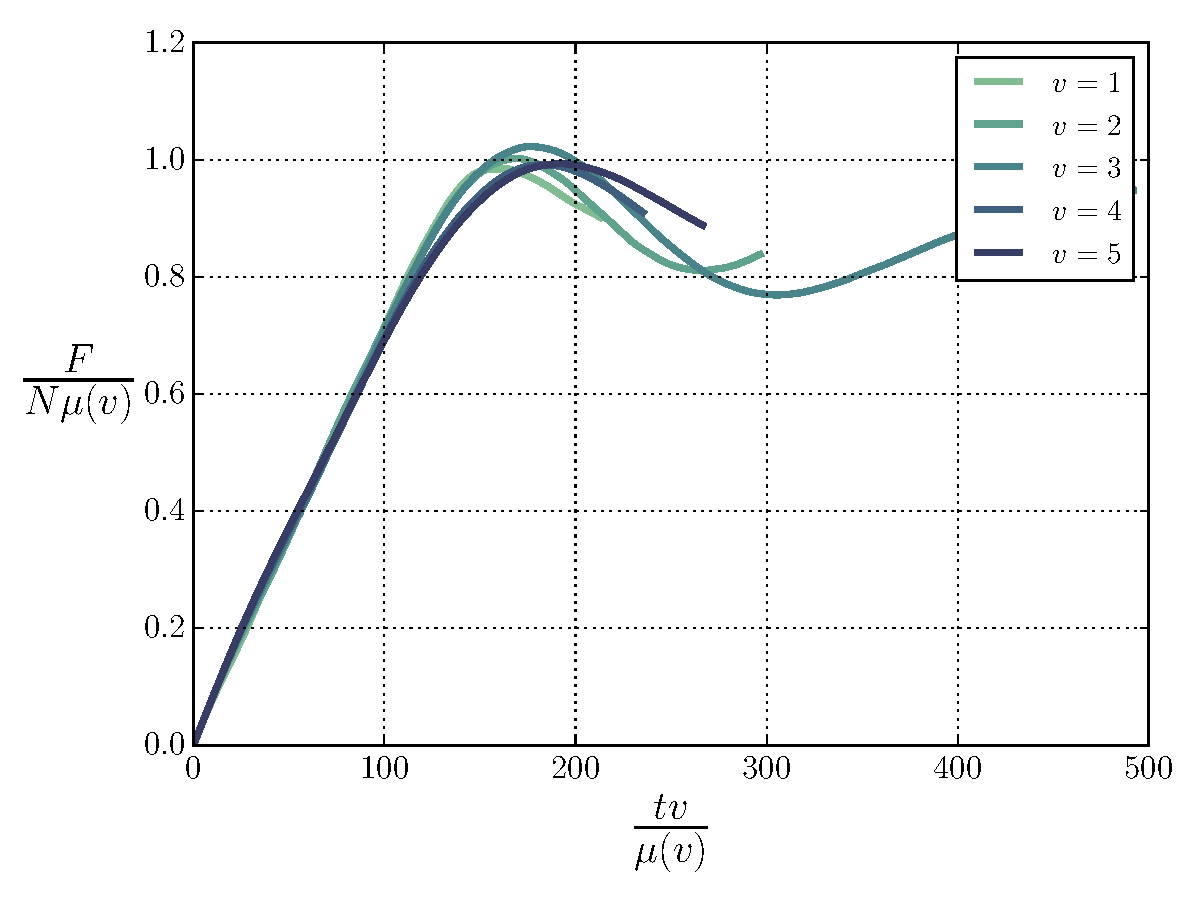
\includegraphics[width=0.7\linewidth]{figures/friction/scalingCoeffisient/dataCollapse}
\caption{Data collapse of series of simulations utilizing different velocities.}
\label{fig:springDataCollapse}
\end{figure}

%As illustrated in figure \ref{fig:steadyslide}, we expect the shear force (spring force) to increase linearly until it has the same magnitude as the static friction force, $F_s$.
%At this point it should decrease as sliding occurs.    


\begin{figure}[H]
	\centering
	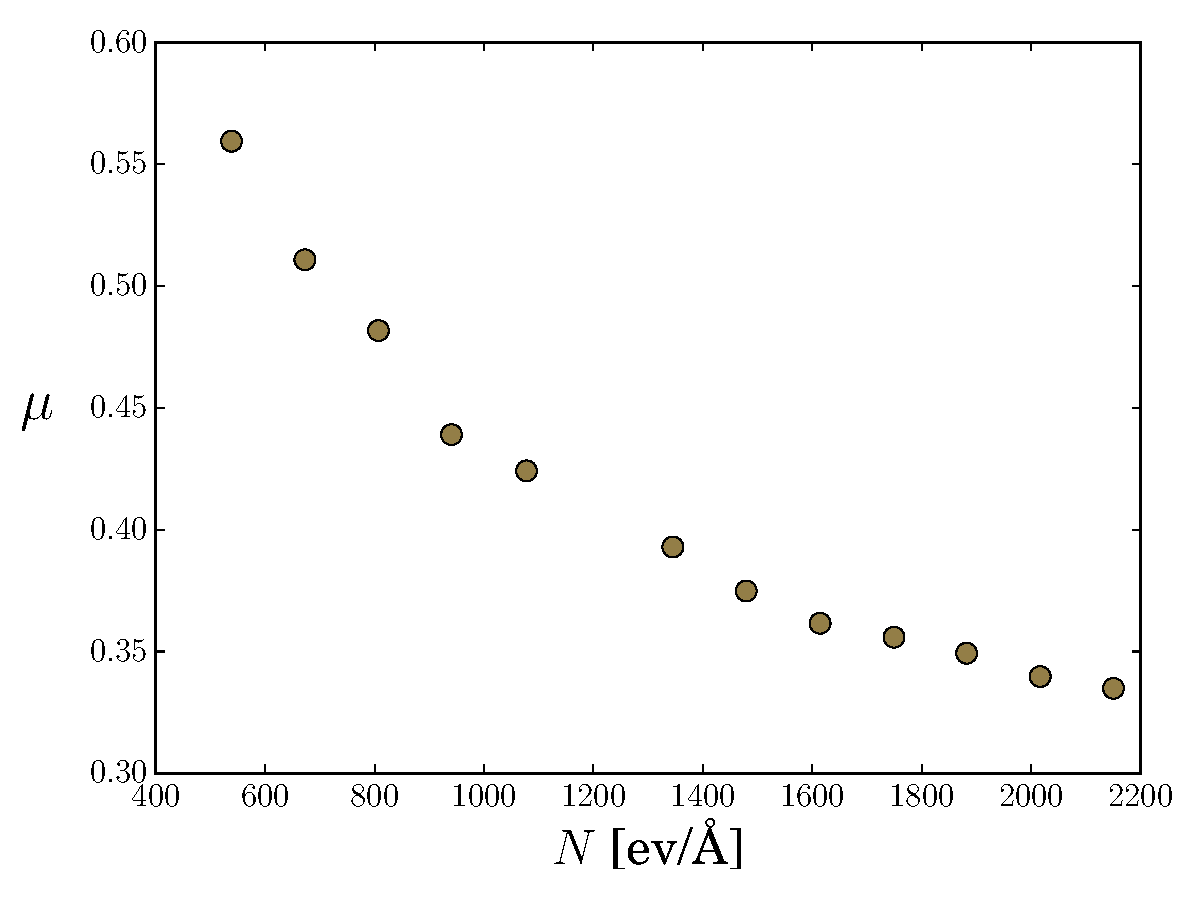
\includegraphics[width=0.7\linewidth]{figures/friction/scalingCoeffisient/UvsN}
	\caption{Coefficient of friction $\mu$ as a function of normal force/load $N$.}
	\label{fig:uvsn}
\end{figure}


\begin{figure}[H]
	\centering
	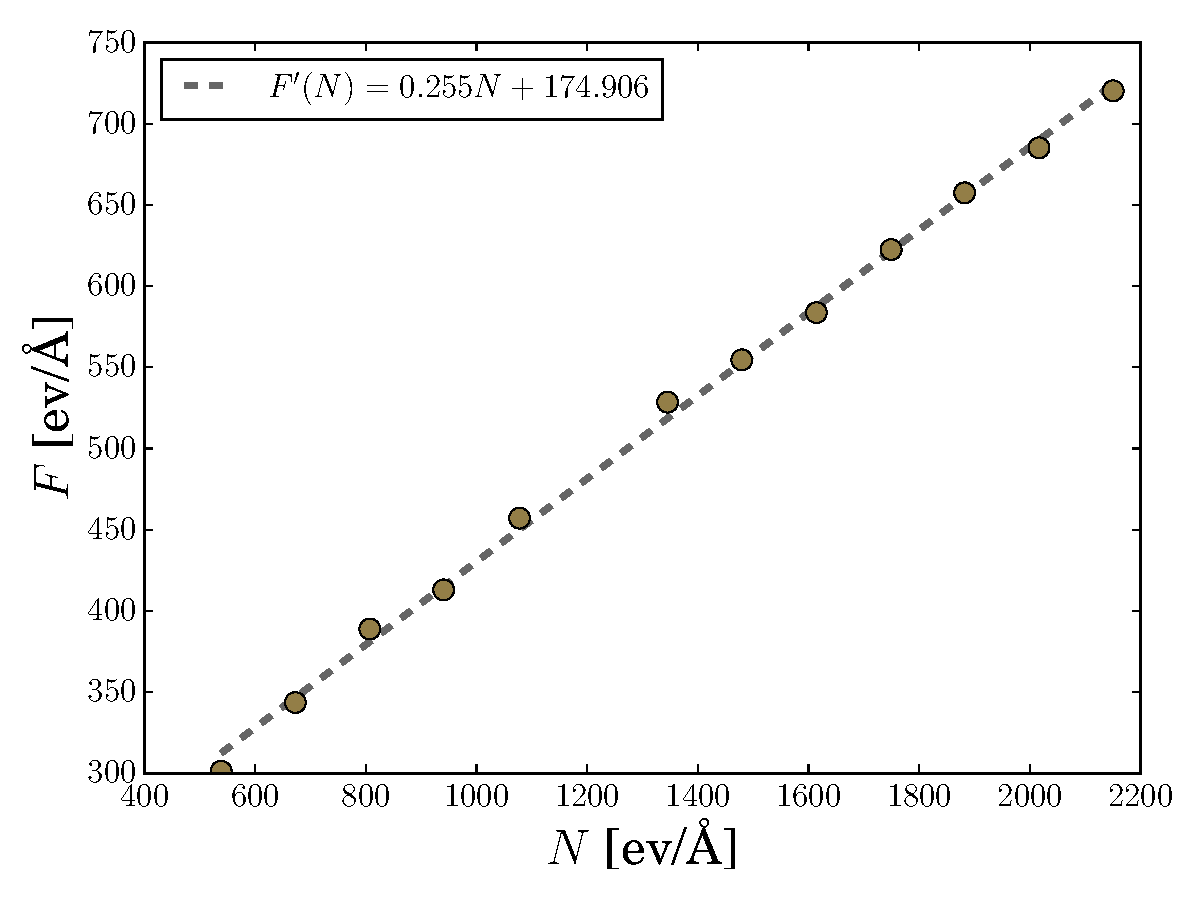
\includegraphics[width=0.7\linewidth]{figures/friction/scalingCoeffisient/FvsN}
	\caption{Shear force $F$ as a function of normal force/load $N$.}
	\label{fig:fvsn}
\end{figure}



\section{Results}
Our prime goal was to find a dependence in the coefficient of static friction on the thickness of the substrate. 
We were therefore obliged to do the same simulation with the simple perturbation of changing the thickness of the substrate. 
The substrate is formed by carving out atoms above a specified z-coordinate, beneath the sphere. 
It is there fore critical to be aware of where we cut the substrate. 
The way the crystalline structure of the substrate was oriented, a difference in 1$\mathring{A}$, would change the upper most layer of atoms of the substrate to be all oxygen or all silicon.
If for one measurement they are all oxygen and another all silicon, we will get very different results. {\huge \color{editColor} Example?}. 
To remove the risk of error, we vary the thickness of the substrate by steps with length of the unit cell (7.12$\mathring{A}$).
For each thickness of the substrate, we estimated the coefficient of static friction using the method described in the previous section of this chapter.
The result is shown in figure \ref{fig:coefficientVsIndentation}.

\begin{figure}[H]
	\centering
	\hspace{-5mm}
	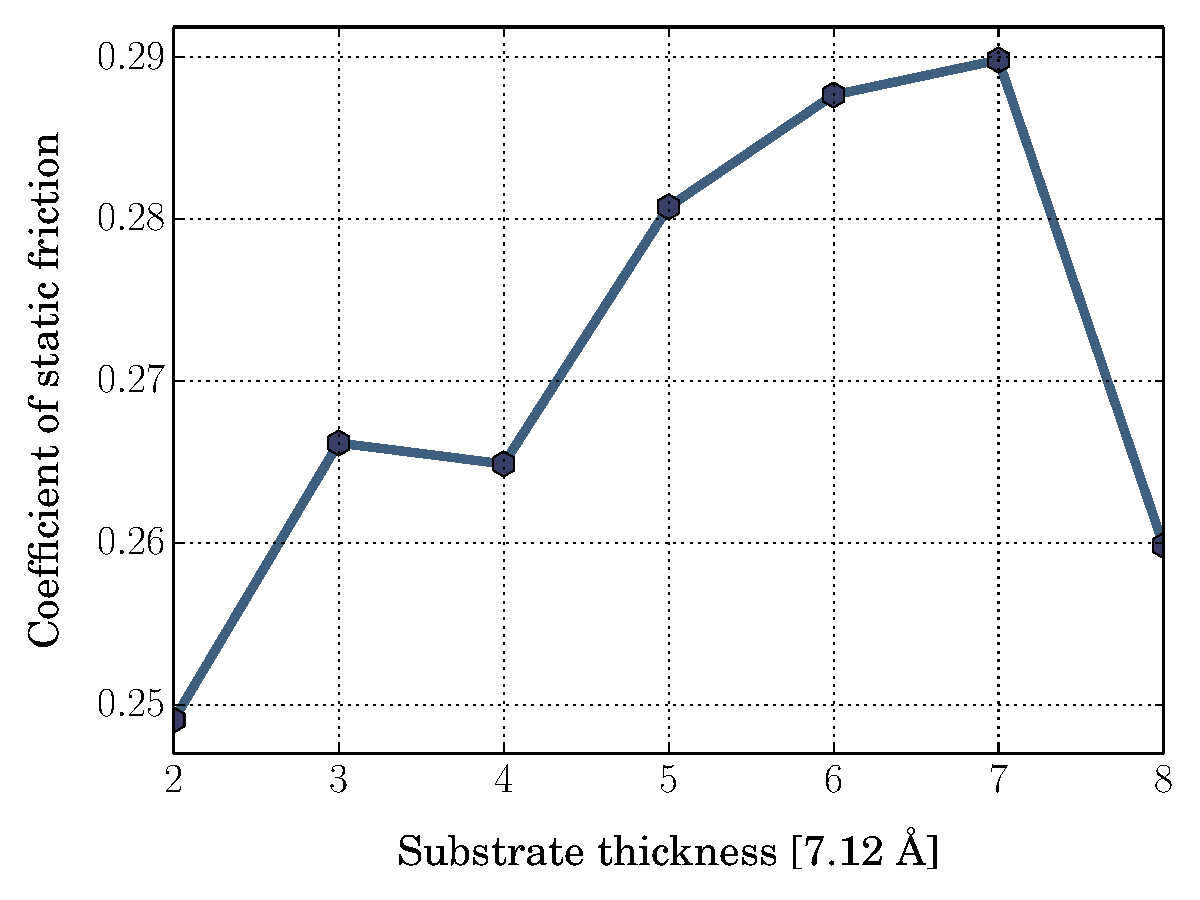
\includegraphics[width=0.7\linewidth]{figures/friction/coefficientVsIndentation}
	\caption{Measured coefficient of static friction for various thicknesses of the substrate. 
		Each measurement is taken as the gradient of a linear approximation as done in illustrated in figure \ref{fig:fvsn}, as defined by Amontons' law. 
		}
	\label{fig:coefficientVsIndentation}
\end{figure}

\noindent
The coefficient of static friction increases with the substrate thickness;
most rapidly at small thicknesses, and less at large thicknesses. 
As the thickness increases the coefficient seems to approach some finite limit. 
From the functional form leading up to final step, we may estimate this limit, which represents the coefficient we would have measured at arbitrary large thickness. 

 



\begin{comment}
\begin{table}[H]
	\begin{center}
		\caption{Measurement results for simulation with substrate of thickness $h=58$\AA. 
			$Step$ is the time step at which the loaded restart file was saved. 
			$k$ is the spring stiffness, 
			$v$ the velocity by which we pull the spring, 
			$N$ the measured normal force, and 
			$F_T$ the force applied to the rigid top of the sphere cap at the time sliding occurs. 
			The units are as described by the $metal$ convention listed 
			in table \ref{tab:unitsMetal}.}
		\begin{tabularx}{0.8\textwidth}{  @{\hspace{2em}} @{}X @{\hspace{-0.5em}}Y@{\hspace{0em}}Y@{\hspace{2em}}XX@{} @{\hspace{0em}} }
			%Measurement			 & unit	\\
			\toprule
			$~Step$ 		&	$k$		&	$v$		&	$~N$		&	$~F_T$ \\
			\midrule
			80000	  &	 10	 	 & -0.1	   &   541	  &   259 \\
			90000	  &	 10	 	 & -0.2	   &   672	  &   391 \\
			100000	 &	10		& -0.2	  &   805	 &   506 \\
			110000	 &	10		& -0.2	  &   942	 &   552 \\
			120000	 &	10		& -0.2	  &   1077	 &   608 \\
			130000	 &	10		& -0.2	  &   1208	 &   731 \\
			140000	 &	10		& -0.2	  &   1341	 &   853 \\
			150000	 &	10		& -0.2	  &   1480	 &   888 \\
			160000	 &	10		& -0.2	  &   1613	 &   936 \\
			170000	 &	10		& -0.2	  &   1745	 &   1142 \\
			180000	 &	10		& -0.2	  &   1881	 &   1400 \\
			190000	 &	10		& -0.2	  &   -	 &   - \\
			200000	 &	10		& -0.2	  &   2150	 &   1502 \\
			
			
			\bottomrule
		\end{tabularx}
		\label{tab:measurements}
	\end{center}
\end{table}
\end{comment}





\part{Discussion}

The normal force distribution does not seem to fit very well with Hertz theory.
Our result is way more linear in $r$. 
The assumptions used in Hertz' theory are (\href{https://en.wikipedia.org/wiki/Contact_mechanics}{wikipedia})
\begin{itemize}
	\item The strains are small and within the elastic limit.
	\item The surfaces are continuous and non-conforming\footnote{
A non-conforming contact is when dissimilar surfaces (which fit badly together) are in contact. When under zero load, they would only touch at a single point. 
The real area of contact is small compared to the sizes of the objects and the stress is highly concentrated.}.
	\item Each body can be considered an elastic half-space.
	\item The surfaces are frictionless.
\end{itemize}

We have not checked if the deformations were elastic throughout the simulation.
We absolutely have friction present.
The hysteresis plot illustrates the presence of adhesion.
It would not be possible do a molecular dynamics simulation and disregard the effects of friction.
 




When measuring the shear force, we did not mind how the substrate was cut, when adjusting the depth of the substrate.
This could cause large differences in the surface properties! 
Since in the one case, the surface has a larger concentration of one type of atom, while in the other case it has a larger concentration of the other type. 



\section{coefficient}
This illustrates a typical technique used in molecular dynamics. 
As in macroscopic experiments we may use way thicker substrates, inadequate for simulations. 
In stead we may look for a behavior and estimate the value from extrapolation of this behavior.


% ---------------------------------------------------------------------------- %

\appendix

\chapter{Something}
\section{LAMMPS units}

\begin{table}[H]
	\begin{center}
		\caption{Unit convention of the \textit{metal} unit style in LAMMPS.}
		\begin{tabularx}{0.8\textwidth}{  @{\hspace{2em}} @{}XX@{} @{\hspace{2em}} }
			%Measurement			 & unit	\\
			\toprule
			Mass 					   & grams/mole\\ 
			\midrule
			Distance 		   		  & Angstroms\\
			\midrule
			Time 				 		& picoseconds\\
			\midrule
			Energy 			   		  & eV\\
			\midrule
			Velocity 		   		  & Angstroms/picosecond\\
			\midrule
			Force 			    	   & eV/Angstrom\\
			\midrule
			Torque 			    	  & eV\\
			\midrule
			Temperature    		  & Kelvin\\
			\midrule
			Pressure 		 		 & bars\\
			\midrule
			Dynamic viscosity & Poise\\
			\midrule
			Charge 					 & multiple of electron charge\\
			\midrule
			Dipole 					 & charge $\cdot$ Angstroms\\
			\midrule
			Electric field 		    & volts $/$ Angstrom\\
			\midrule
			Density 				& gram $/$ cm\^{}dim\\
			\bottomrule
		\end{tabularx}
		\label{tab:unitsMetal}
	\end{center}
\end{table}

\section{Building LAMMPS with custom compute}
In order to use the custom compute \texttt{group/group/atom}, some files in the lammps distribution must be perturbed.  
All files that have been altered during this thesis are available at my githuh-account in the directory named \textit{modifiedLammpsFiles}.  
The compute uses only the two-body part of the potential. 
As a consequence, we must set the \texttt{single\_enable}-flag to be true in \texttt{pair\_vashishta.cpp}. 
Also
terminal commands for building LAMMPS again?



\bibliographystyle{plain}
\bibliography{resources/Library.bib}


%Referances






\end{document}
```

Centering the front page
------------------------
By default, the maketitle command will generate the front page, but it will not be properly centered, but offset like any other page. To get around this, the best solution is to create a separate document, name it front-page.tex and add the following to it:

front-page.tex:
```latex
\documentclass[twoside,english]{uiofysmaster}
\geometry{a4paper,includeall,bindingoffset=0cm,margin=3cm,
            marginparsep=0cm,marginparwidth=0cm,top=2cm}

\author{Filip Henrik Larsen}
\title{\uppercase{The history of master thesises and other random gibberish}}
\date{June 2012}

\begin{document}

\begin{titlepage}
\maketitle
\end{titlepage}

\end{document}
